\documentclass[a4paper,12pt,twoside]{report}
% VARIABLES

\newcommand{\titulo}{Programación básica y Programación de algoritmos paralelos con CUDA} % Título completo
\newcommand{\titred}{Porgramación con CUDA} % Título corto
\newcommand{\periodo}{\today} % Año academico
\newcommand{\institucion}{Universidad de Santiago de Compostela} % Universidad
\newcommand{\carrera}{Ingeniería Informática} % Grado
\newcommand{\asignatura}{Programación de Arquitecturas Emergentes} % Asignatura
\newcommand{\autor}{Jorge Lojo Abal} % Autor del documento
%\newcommand{\autorii}{}
\newcommand{\autores}{Pablo Liste Cancela, \autor} % Autores completos


% PAQUETES, ENTORNOS Y ESTILO DEL DOCUMENTO
\usepackage[spanish,es-tabla]{babel} % Tildes
\usepackage[utf8]{inputenc}          % Símbolos

% Formato de texto
\usepackage{titlesec}   % Formato de títulos
\usepackage{multicol}   % Múltiples columnas
\usepackage{geometry}   % Disposición página
\usepackage{parskip}    % Control interpárrafo
\usepackage{xcolor}     % Referencias de color
\usepackage{enumitem}   % Control de listas
\usepackage{fancyhdr}   % Encabezados y pies
\usepackage{hyperref}   % Enlaces
\usepackage{authblk}    % Posible footnote style en autor
\usepackage{lmodern}    % Fuentes latinas
\usepackage[outputdir=./.ltxaux]{minted} % Bloques código
\usepackage{datetime2}
%\usepackage{iftex}      % Saver si es TeX, LaTeX, etc
%\usepackage{bold-extra} % Negrita en versalitas

% Figuras y entornos
\usepackage{graphicx}   % Incluir fotos
\usepackage{caption}    % Descripciones figuras
\usepackage{subcaption} % Extensión a subfiguras
\usepackage{adjustbox}  % Ajuste y control boxes
%\usepackage{wrapfig}    % Figuras/tablas con texto al lado

% Matemático y símbolos
\usepackage{amsmath}    % Fórmulas
\usepackage{mathrsfs}   % Fuentes
\usepackage{wasysym}    % Algunos wasy fonts y simbolos
\usepackage{amssymb}    % Más simbolos
%\usepackage[official]{eurosym} % Símbolo euro

% TABLAS
\usepackage{tabulary}       % Tabla con columnas dinámicas
\usepackage{array}          % Extensión de tablas
\usepackage{booktabs}       % Mejor formateo agua
\usepackage{hhline}         % Hlines mas dinamico
\usepackage{colortbl}       % Celdas coloreadas
\usepackage{arydshln}       % Líneas punteadas
\usepackage{vcell}          % Alineado vertical celdas   
\usepackage{threeparttable} % Notas despues de la tabla
\usepackage{multirow}       % Unir celdas
\usepackage{listings}

%General
%\usepackage{lipsum}

%Gestión de anexos
%\usepackage{appendix}

\usepackage{verbatim}
\usepackage[T1]{fontenc}
\usepackage{tikz}
\usepackage{float}
\usepackage{comment}
\usepackage{makeidx}
\usepackage{url}
\usepackage{lastpage}
\usepackage{bookmark}
\usepackage{listings}
\usepackage{lstautogobble}
\usepackage{longtable}
\selectlanguage{spanish}

% ANEXOS
%\renewcommand{\appendixname}{Anexos}
%\renewcommand{\appendixtocname}{Anexos}
%\renewcommand{\appendixpagename}{Anexos}

% BIBLIOGRAFIA
%\AtBeginDocument{
%  \renewcommand{\bibsection}{\chapter{\bibname}}
%} % Bibliografia en capitulo numerado

%\captionsetup{hypcap=true}

% COLORES
\definecolor{shadecolor}{gray}{0.95}

% Parrafos en el indice
\setcounter{secnumdepth}{4}
\setcounter{tocdepth}{4}



%MÁRGENES
\setlength{\headheight}{15pt}
\geometry{top=2.54cm, bottom=4cm, left=2.54cm, right=2.54cm}
\parindent=12.7mm
\headsep=15mm
\footskip=15mm

%ENCABEZADOS Y PIES
\pagestyle{fancy}
\fancyhf{}
\fancyhead[LE,RO]{\rightmark}
\fancyhead[RE,LO]{\titred}
\fancyfoot[CE,CO]{\leftmark}
\fancyfoot[LE,RO]{\thepage}
\renewcommand{\headrulewidth}{0pt}
\renewcommand{\footrulewidth}{0.pt}

%INFORMACIÓN DOCUMENTO
\title{\titulo}
\author{\autores}
\affil{\asignatura\\ \institucion\\ \carrera}
\date{\periodo}

% FECHAS
\DTMnewdatestyle{mesanyo}{%
  \renewcommand{\DTMdisplaydate}[4]{%
    \DTMspanishMonthname{##2} ##1%
  }%
}
\DTMsetdatestyle{mesanyo}

\graphicspath{ {imagenes/} }

% CAPITULOS SIN 'CAPITULO'
\titleformat{\chapter}[hang]{\Huge\bfseries}{\thechapter.}{1em}{\LARGE}


\setlength{\headheight}{16pt}
\addtolength{\topmargin}{-1pt}

% Metadatos
\hypersetup{ 
    pdfauthor={\autor} % Autor del trabajo
    pdftitle={\titulo} % Título del trabajo
    pdfsubject={} % Memoria del proyecto
    pdfkeywords{} % Palabras clave del documento
    pdflang={español} % Idioma del documento
    pdfcreator={\autor} % Creador del documento
}

\begin{document}

    % PORTADA

    \maketitle

    % ÍNDICE

    \begingroup
        \hypersetup{linkcolor=black}

        \tableofcontents
    \endgroup
    
    \newpage
    
    % INTRODUCCION
    \chapter{Introducción}

En el panorama actual de la computación de alto rendimiento, la programación paralela en sistemas de memoria compartida se ha convertido en un componente fundamental para el aprovechamiento eficiente de las arquitecturas \textit{multicore} modernas. El paradigma de programación OpenMP (\textit{Open Multi-Processing}) destaca como una solución estándar y portable que permite explotar el paralelismo a nivel de hilo en procesadores multinúcleo, facilitando el desarrollo de aplicaciones que pueden beneficiarse de la ejecución concurrente. En este contexto, la presente práctica se centra en la \textbf{Programación Básica y Programación de Algoritmos Paralelos con OpenMP}, constituyendo el tercer bloque del laboratorio dentro de la asignatura de \textbf{Programación de Arquitecturas Emergentes} del Grado en Ingeniería Informática.

El objetivo principal de esta práctica es adquirir los conocimientos fundamentales para la implementación de programas paralelos en sistemas de memoria compartida y aplicar las metodologías de programación paralela estudiadas en clase utilizando OpenMP. Las actividades se desarrollarán en los nodos de cómputo del \textbf{Centro de Supercomputación de Galicia} (CESGA), específicamente en el sistema \texttt{FTIII} que proporciona nodos con 64 \textit{cores}, representando un entorno ideal para la experimentación con diferentes configuraciones de paralelismo a nivel de hilo.

A diferencia de prácticas anteriores centradas en algoritmos secuenciales o en la programación con CUDA para GPUs, este trabajo aborda la implementación y optimización de algoritmos fundamentales que exploran diferentes características de OpenMP y patrones de paralelismo en CPUs \textit{multicore}. La estructura de la práctica se divide en dos bloques principales que abordan progresivamente diferentes aspectos del paralelismo con OpenMP:

\begin{itemize}

    \item \textbf{Bloque 1: Programación básica con OpenMP}: Este bloque se enfoca en comprender los fundamentos de OpenMP, explorando aspectos como el comportamiento por defecto del \textit{scheduling} y \textit{chunk size} en distintos compiladores, el estudio de los \textit{pragmas} esenciales como \texttt{reduction}, \texttt{collapse}, \texttt{task} y \texttt{taskloop} asi como la implementación de técnicas de reparto de trabajo para la inicialización eficiente de matrices de gran tamaño.

    \item \textbf{Bloque 2: Programación de algoritmos paralelos con OpenMP}: En este bloque se implementarán dos algoritmos fundamentales con diferentes patrones de acceso a memoria y requisitos de paralelismo:

    \begin{itemize}
    
        \item \textbf{Distancia Euclídea}: Un algoritmo que requiere operaciones de reducción, implementado tanto con la cláusula \texttt{reduction} nativa de OpenMP como con una versión propia para comparar su eficiencia. Se analizará el tipo de escalabilidad (fuerte o débil) para determinar cómo responde el algoritmo ante diferentes configuraciones.

        \item \textbf{Convolución}: Un algoritmo con patrones de acceso regular pero intensivo en cómputo, utilizado ampliamente en procesamiento de señales e imágenes. Se evaluará su aceleración (\textit{speedup}) al variar el número de hilos y se explorarán diferentes estrategias de optimización.
        
    \end{itemize}

\end{itemize}

La arquitectura multinúcleo del sistema \texttt{FTIII} proporciona un escenario ideal para estas implementaciones, permitiendo experimentar con un gran número de \textit{cores} en un entorno de memoria compartida. Esta configuración \textit{hardware} posibilita explorar los límites reales del paralelismo a nivel de hilo y evaluar cómo diferentes decisiones de diseño en la programación con OpenMP afectan al rendimiento final de los algoritmos.

Este estudio no solo busca lograr implementaciones eficientes, sino también comprender en profundidad cómo las características arquitectónicas de los procesadores multinúcleo modernos y las opciones de configuración de OpenMP influyen en el rendimiento de diferentes patrones algorítmicos. Se analizarán aspectos críticos como la configuración óptima de \textit{scheduling} y \textit{chunk size}, las políticas de reparto de iteraciones, el balance de carga entre hilos, y la comparación entre diferentes \textit{pragmas} de paralelismo como \texttt{parallel for} frente a \texttt{taskloop}.

Los resultados obtenidos se documentarán mediante un análisis comparativo, abarcando diversas métricas clave que permitan evaluar el rendimiento y la eficiencia de las implementaciones desarrolladas. En particular, se medirán los factores de aceleración (\textit{speedup}) con respecto a ejecuciones secuenciales optimizadas, utilizando diferentes configuraciones de hilos (2, 4, 8, 16, 32, 48 y 64), y se analizarán por separado tanto el rendimiento global como el de los \textit{kernels} computacionales específicos.

Además, se estudiarán en profundidad los patrones de concurrencia y su relación con la arquitectura subyacente, explorando cómo la topología del procesador (visualizada con herramientas como \texttt{lstopo}) influye en el desempeño de las implementaciones paralelas. Se evaluará la eficiencia en la utilización de los recursos computacionales y se explorarán posibles cuellos de botella que puedan surgir en la ejecución, junto con estrategias para mitigarlos.

Finalmente, se discutirán las observaciones y conclusiones derivadas de la experimentación con distintas configuraciones de ejecución, proporcionando una visión integral sobre la programación eficiente con OpenMP en sistemas de memoria compartida. Este análisis permitirá no solo validar la efectividad de las estrategias implementadas, sino también extraer pautas generales para el desarrollo de algoritmos paralelos altamente optimizados en arquitecturas \textit{multicore} modernas.
    \chapter{Entorno de ejecución}

Para llevar a cabo este estudio, los algoritmos paralelos serán implementados y ejecutados en el supercomputador FinisTerrae III del Centro de Supercomputación de Galicia (CESGA), aprovechando su arquitectura multinúcleo para evaluar el rendimiento de las implementaciones con OpenMP.

El FinisTerrae III, instalado en el año 2021 y puesto en producción en el año 2022, es un supercomputador modelo Bull ATOS bullx distribuido en 13 \textit{racks} con un total de 354 nodos de computación. Este sistema de alto rendimiento dispone de 22656 núcleos Intel Xeon Ice Lake 8352Y, junto con 128 GPUs NVIDIA A100 y 16 NVIDIA T4 para aceleración de cómputo. Para nuestros experimentos con OpenMP, resultan particularmente relevantes los nodos estándar equipados con procesadores Intel Xeon, que ofrecen características excepcionales para computación paralela en memoria compartida:

\begin{itemize}

    \item \textbf{Procesadores}: 2 procesadores Intel Xeon Ice Lake 8352Y por nodo de computación.
    
    \item \textbf{Núcleos físicos}: 64 \textit{cores} por nodo (32 \textit{cores} por \textit{socket}).
    
    \item \textbf{Jerarquía de caché}: Tres niveles con caché L1 y L2 dedicadas por \textit{core}, y una L3 compartida que mejora el rendimiento en aplicaciones paralelas con datos compartidos.
    
    \item \textbf{Instrucciones vectoriales}: Soporte para conjuntos de instrucciones AVX-512, que permiten procesamiento vectorial optimizado de datos en punto flotante.
    
\end{itemize}

La interconexión entre nodos se realiza mediante una red Mellanox Infiniband HDR de baja latencia y alta velocidad, crucial para aplicaciones distribuidas, aunque en nuestra práctica nos centraremos principalmente en el paralelismo a nivel de hilo dentro de un único nodo aprovechando la arquitectura de memoria compartida. El sistema de almacenamiento Lustre con 5000 TB proporciona el espacio necesario para los conjuntos de datos y resultados experimentales, con un rendimiento optimizado para operaciones de Entrada/Salida intensivas.

Con una capacidad máxima de cómputo teórica de 4 PetaFlops, el FinisTerrae III representa un entorno ideal para la evaluación de algoritmos paralelos, permitiéndonos analizar el comportamiento de implementaciones OpenMP bajo condiciones de alta disponibilidad de recursos computacionales.

\newpage

\section{Consideraciones}
	
Todos los experimentos se realizarán siguiendo estas pautas:
    
\begin{itemize}

    \item Desarrollo inicial en nodos interactivos para depuración y pruebas (\texttt{compute}).
    
    \item Mediciones finales en nodos completos con 64 \textit{cores} mediante el sistema de colas SLURM, utilizando la cola \texttt{short}.
    
    \item Compilación con optimizaciones \texttt{-O2} tanto con el compilador GNU GCC como con el compilador Intel ICC para comparar rendimiento.
    
    \item Tiempo de ejecución calculado como media de 10 ejecuciones para mitigar variabilidad estadística.
    
    \item Separación explícita del \textit{overhead} de gestión de memoria (\textit{malloc}, \textit{free}, inicialización) del tiempo de ejecución de los algoritmos paralelos.
    
    \item Exploración sistemática de diferentes políticas de \textit{scheduling} (\textit{static}, \textit{dynamic}, \textit{guided} y \textit{auto}) y tamaños de \textit{chunk}.
    
    \item Análisis de la topología del procesador utilizando la herramienta \texttt{lstopo} para optimizar el comportamiento según la disposición NUMA.
    
    \item Verificación exhaustiva de la corrección de resultados mediante comparación con implementaciones secuenciales.
    
    \item Mediciones de métricas de rendimiento como \textit{speedup} con 2, 4, 8, 16, 32, 48 y 64 hilos para evaluar la escalabilidad.
    
\end{itemize}
	
Los experimentos se han dimensionado considerando las restricciones de tiempo impuestas por el sistema de colas del supercomputador, particularmente el límite de 2 horas en la cola corta, lo que ha condicionado tanto el tamaño de los conjuntos de datos como el número de configuraciones evaluadas.
    \chapter{Ejercicio 1: Inicialización de matriz}

\section{Introducción}

    En este apartado se presenta un análisis detallado del rendimiento y la ocupancia de un \textit{kernel} CUDA diseñado para inicializar una matriz de números secuenciales de tamaño 1 GiB. El objetivo principal es determinar la configuración óptima de hilos y bloques para maximizar el rendimiento en una GPU NVIDIA A100, explorando sistemáticamente diferentes configuraciones para identificar patrones y establecer recomendaciones fundamentadas para futuras implementaciones.
    
    La inicialización de matrices es una operación fundamental en computación paralela y, aunque aparentemente simple, permite explorar aspectos clave del rendimiento en GPUs como la organización de hilos, la ocupancia de los multiprocesadores y los patrones de acceso a memoria. Este análisis proporciona \textit{insights} valiosos sobre cómo la arquitectura de la GPU influye en el rendimiento de operaciones paralelas básicas.
    
    El estudio se ha realizado siguiendo metodologías rigurosas de medición y análisis, abarcando 33 configuraciones diferentes de bloques que varían tanto en tamaño como en forma, lo que permite una exploración exhaustiva del espacio de posibilidades de paralelización.

\newpage

\section{Descripción de la implementación}

    El \textit{kernel} implementado inicializa una matriz de enteros de 1 GiB con valores secuenciales de la forma \texttt{fila*N+columna}. La parte principal del \textit{kernel} es:

    \begin{listing}[h]
        \begin{minted}[frame=single,linenos, breaklines, fontsize=\normalsize]{c}
__global__ void initMatrix(int* matrix, size_t M, size_t N) {
        
    // Calculate global thread indices
    size_t col = blockIdx.x * blockDim.x + threadIdx.x;
    size_t row = blockIdx.y * blockDim.y + threadIdx.y;

    // Check if thread is within matrix bounds
    if (row < M && col < N) {

        size_t idx = row * N + col;
        matrix[idx] = row * N + col;

    }

}
        \end{minted}
        \caption{Kernel de inicialización.}
    \end{listing}
    
    \subsection{Características principales del código}

        El código implementado presenta las siguientes características fundamentales:
        
        \begin{itemize}

            \item \textbf{Paralelización bidimensional}: Utiliza una organización de hilos y bloques bidimensional para ``mapear'' naturalmente la estructura de la matriz.
            
            \item \textbf{Cálculo de índices globales}: Determina la posición global de cada hilo dentro de la matriz mediante la combinación de los índices de bloque y de hilo.

            \item \textbf{Comprobación de límites}: Incorpora una verificación de límites para asegurar que los hilos no accedan a posiciones fuera de la matriz, lo que es crucial cuando el número de hilos no es un divisor exacto de las dimensiones de la matriz.
            
            \item \textbf{Acceso a memoria linealizado}: Convierte los índices bidimensionales en un índice lineal para acceder a la memoria global de manera eficiente.
            
            \item \textbf{Patrón de escritura regular}: Cada hilo escribe exactamente un valor en la matriz, siguiendo un patrón regular que facilita la coalescencia de accesos a memoria.
            
            \item \textbf{Ausencia de sincronización}: El \textit{kernel} no requiere sincronización entre hilos, lo que elimina posibles cuellos de botella relacionados con la coordinación.
            
            \item \textbf{Adaptabilidad a diferentes configuraciones}: El código está diseñado para funcionar con cualquier configuración de hilos por bloque, permitiendo una exploración exhaustiva del espacio de configuraciones.
            
        \end{itemize}
        
    \subsection{Consideraciones de diseño}
    
        Al diseñar este \textit{kernel}, se tuvieron en cuenta varias consideraciones importantes:

        \begin{itemize}
        
            \item \textbf{Simplicidad computacional}: La operación de inicialización es aritméticamente simple (una multiplicación y una suma), lo que hace que el \textit{kernel} esté probablemente limitado por el acceso a memoria más que por el poder computacional.
            
            \item \textbf{Patrón de acceso a memoria}: Se intentó mantener un patrón de acceso a memoria que favoreciera la coalescencia, donde hilos adyacentes acceden a posiciones de memoria contiguas.
            
            \item \textbf{Tamaño de problema considerable}: Con 1 GiB de datos (268435456 elementos de 4 bytes), el problema es lo suficientemente grande como para ejercitar completamente la GPU y obtener mediciones significativas al mismo tiempo que no ve lastrado el proceso de evaluación por un tamaño de problema excesivo.
            
            \item \textbf{Flexibilidad en la configuración}: El \textit{kernel} está diseñado para funcionar con cualquier configuración de bloques, lo que permite evaluar el impacto de diferentes organizaciones de hilos en el rendimiento.
            
        \end{itemize}

\newpage

\section{Fundamentos teóricos}

    \subsection{Cálculo del número de elementos}

        Para una matriz que ocupe exactamente 1 GiB de memoria, como se solicita en el enunciado de la práctica, necesitamos realizar las siguientes operaciones:
        
        \begin{align*}
            \text{1 GiB} &= 2^{30} \text{bytes} = 107341824 \text{bytes}.\\
            \text{Tamaño de un entero} &= 4 \text{bytes}.\\
            \text{Número total de elementos} &= \frac{1073741824 \text{bytes}}{4 \text{bytes/elemento}} = 268435456 \text{elementos}.
        \end{align*}
        
        Para obtener una matriz cuadrada que contenga el número de elementos necesario, realizamos los siguientes cálculos:
        
        \begin{align*}
            M \times N &= 268435456.\\
            M &= N = \sqrt{268435456} = 16384.
        \end{align*}

        Por lo tanto, una matriz cuadrada de 16384×16384 elementos de tipo entero ocupan exactamente 1 GiB de memoria. Este tamaño es importante porque permite explorar el comportamiento del \textit{kernel} con una carga de trabajo sustancial, poniendo a prueba la capacidad de la GPU para gestionar grandes volúmenes de datos.
        
        Es importante destacar que la elección de una matriz cuadrada no es arbitraria. Las matrices cuadradas suelen facilitar la implementación de algoritmos paralelos al permitir una distribución más regular del trabajo entre los hilos. Además, en aplicaciones reales de computación científica y procesamiento de imágenes, las matrices cuadradas son comunes, lo que hace que este análisis sea relevante para casos de uso prácticos.

    \subsection{Modelo de ejecución CUDA y organización de hilos}

        El modelo de ejecución CUDA organiza los hilos en una jerarquía de tres niveles:

        \begin{itemize}
        
            \item \textbf{Hilos (\textit{Threads})}: La unidad básica de ejecución. Cada hilo ejecuta el mismo código (\textit{kernel}) pero opera sobre diferentes datos.
            
            \item \textbf{Bloques (\textit{Blocks})}: Agrupaciones de hilos que se ejecutan en el mismo SM y pueden cooperar mediante memoria compartida y sincronización. Los bloques se asignan a SMs específicos y no pueden migrar entre ellos durante la ejecución.
            
            \item \textbf{\textit{Grid}}: Conjunto de bloques que ejecutan el mismo \textit{kernel}. Representa la totalidad del trabajo a realizar.
            
        \end{itemize}
        
        Los hilos dentro de un bloque se organizan en \textit{warps} de 32 hilos, siendo el \textit{warp} la unidad básica de ejecución física en las GPUs NVIDIA. Todos los hilos de un \textit{warp} ejecutan la misma instrucción simultáneamente siguiendo el modelo \textbf{SIMT} (\textit{Single Instruction}, \textit{Multiple Threads}).
        
        \subsubsection{Implicaciones del modelo SIMT}
    
            El modelo SIMT tiene implicaciones importantes para el rendimiento:
    
            \begin{itemize}
              
                \item \textbf{Divergencia de \textit{warps}}: Si los hilos dentro de un \textit{warp} toman diferentes caminos de ejecución debido a condiciones if-else, se produce una divergencia, lo que reduce la eficiencia puesto que los diferentes caminos deben ejecutarse secuencialmente.
               
                \item \textbf{Coalescencia de memoria}: Cuando los hilos de un \textit{warp} acceden a posiciones de memoria contiguas, estos accesos pueden combinarse en una única transacción de memoria, mejorando significativamente el rendimiento.
                
                \item \textbf{Sincronización implícita}: Los hilos dentro de un \textit{warp} están implícitamente sincronizados, lo que puede aprovecharse para optimizar ciertos algoritmos.
                
            \end{itemize}
            
            Para una matriz bidimensional, la organización de hilos sigue típicamente un patrón 2D, donde:
            
            \begin{align*}
                \text{Índice global columna} &= \text{blockIdx.x} \times \text{blockDim.x} + \text{threadIdx.x}.\\
                \text{Índice global fila} &= \text{blockIdx.y} \times \text{blockDim.y} + \text{threadIdx.y}.
            \end{align*}
            
            Y la posición lineal en memoria se calcula como:
            
            \begin{align*}
                \text{Índice lineal} &= \text{fila} \times N + \text{columna}.
            \end{align*}
            
            Esta organización permite una correspondencia directa entre la estructura bidimensional de la matriz y la estructura bidimensional de los bloques e hilos en CUDA.
                
    \subsection{Cálculo teórico de la ocupancia}
    
        La ocupancia en CUDA se define como la relación entre el número de \textit{warps} activos y el número máximo de \textit{warps} que pueden estar activos en un SM (\textit{Streaming Multiprocessor}). Es un factor crítico para el rendimiento, ya que una alta ocupancia permite a la GPU ocultar mejor las latencias de memoria y mantener sus unidades de cómputo ocupadas logrando mejores resultados en lo referente a los tiempos de ejecución de un \textit{kernel}.
        
        Para poder obtener la ocupancia de nuestras configuraciones podemos calcularla siguiendo la siguiente formula:
        
        \begin{align*}
            \text{Ocupancia} = \frac{\text{Bloques activos por SM} \times \text{\textit{Warps} por bloque}}{\text{\textit{Warps} máximos por SM}}.
        \end{align*}
        
        Donde:
        
        \begin{itemize}
        
            \item \textbf{Bloques activos por SM:} Número de bloques que pueden ejecutarse simultáneamente en un SM.
           
            \item \textbf{\textit{Warps} por bloque:} $\lceil \frac{\text{Hilos por bloque}}{32} \rceil$ (el número de hilos por bloque dividido por 32, redondeado hacia arriba).
           
            \item \textbf{\textit{Warps} máximos por SM:} 64 en la GPU A100 (equivalente a 2048 hilos / 32 hilos por \textit{warp}).
        
        \end{itemize}
        
        \subsubsection{Factores que limitan la ocupancia}

            El número de bloques activos por SM está limitado por varios factores:
            
            \begin{itemize}
                
                \item \textbf{Límite de bloques por SM:} 32 bloques en la arquitectura A100.
               
                \item \textbf{Límite de hilos por SM:} 2048 hilos en la arquitectura A100.
                
                \item \textbf{Límite de registros:} Calculado como $\frac{\text{Registros totales por SM}}{\text{Registros por hilo} \times \text{Hilos por bloque}}$.
                
                \item \textbf{Límite de memoria compartida:} Calculado como $\frac{\text{Memoria compartida por SM}}{\text{Memoria compartida por bloque}}$.
            
            \end{itemize}
            
            El número máximo de bloques activos por SM será el mínimo de estos cuatro límites:

            \begin{align*}
                \text{Bloques SM} = \min(\text{Lim. bloques}, \text{Lim. hilos}, \text{Lim. registros}, \text{Lim. mem. compartida})
            \end{align*}
            
        \subsubsection{Impacto de la ocupancia en el rendimiento}
            
            La relación entre ocupancia y rendimiento no es siempre directamente proporcional. Algunas consideraciones importantes son:
        
            \begin{itemize}
                
                \item \textbf{Ocupancia saturada}: A partir de cierto punto (típicamente 50-70\%), aumentar la ocupancia puede no traducirse en mejoras significativas de rendimiento, ya que otros factores como el ancho de banda de memoria pueden convertirse en el cuello de botella principal.
                
                \item \textbf{Compromiso entre ocupancia y recursos por hilo}: Aumentar la ocupancia puede requerir reducir los recursos por hilo (registros, memoria compartida), lo que puede penalizar el rendimiento si el \textit{kernel} necesita estos recursos.
        
                \item \textbf{Latencia de memoria vs. ocupancia}: Una alta ocupancia es especialmente beneficiosa para \textit{kernels} limitados por latencia de memoria, ya que permite a la GPU alternar entre diferentes \textit{warps} mientras espera datos de memoria.
            
            \end{itemize}
            
            Estas fórmulas y consideraciones muestran que, para nuestro \textit{kernel} de inicialización de matriz, teóricamente podríamos alcanzar una ocupancia del 100\% con bloques desde 64 hasta 1024 hilos, aunque el número de bloques activos por SM varía significativamente según el tamaño del bloque.
        
    \subsection{Cálculo de bloques por SM}
    
        Para cada configuración de bloque, CUDA nos permite calcular el número máximo de bloques que pueden residir en un SM. Esto se realiza haciendo uso de la función \texttt{cudaOccupancyMaxActiveBlocksPerMultiprocessor}, que tiene en cuenta:

        \begin{itemize}
        
            \item \textbf{Tamaño del bloque (número de hilos)}: A mayor número de hilos por bloque, menor número de bloques pueden residir simultáneamente en un SM.
            
            \item \textbf{Uso de registros por hilo}: Cada hilo consume registros, y el número total de registros disponibles por SM es limitado (65536 en la A100).
            
            \item \textbf{Uso de memoria compartida por bloque}: La memoria compartida por SM también es limitada (164 KB en la A100).
            
            \item \textbf{Limitaciones arquitectónicas de la GPU}: Incluyen el máximo de hilos por SM (2048) y el máximo de bloques por SM (32).
            
        \end{itemize}
        
        \subsubsection{Cálculo de bloques por SM}

            Para nuestro \textit{kernel} de inicialización, podemos calcular teóricamente el número máximo de bloques por SM para diferentes tamaños de bloque:
            
            \begin{itemize}

                \item \textbf{Para bloques de 1024 hilos (32 \textit{warps}):}
                
                    \begin{align*}
                        \text{Bloques por SM (hilos)} &= \left\lfloor \frac{2048 \text{hilos/SM}}{1024 \text{hilos/bloque}} \right\rfloor = 2 \text{bloques/SM}\\
                        \text{Bloques por SM (warps)} &= \left\lfloor \frac{64 \text{warps/SM}}{32 \text{warps/bloque}} \right\rfloor = 2 \text{bloques/SM}\\
                        \text{Bloques por SM (límite)} &= 32 \text{bloques/SM}
                    \end{align*}
                    
                    Por lo tanto, el factor limitante es el número de hilos/\textit{warps}, permitiendo 2 bloques por SM.
            
                \item \textbf{Para bloques de 512 hilos (16 warps):}
    
                    \begin{align*}
                        \text{Bloques por SM (hilos)} &= \left\lfloor \frac{2048 \text{hilos/SM}}{512 \text{hilos/bloque}} \right\rfloor = 4 \text{bloques/SM}\\
                        \text{Bloques por SM (warps)} &= \left\lfloor \frac{64 \text{warps/SM}}{16 \text{warps/bloque}} \right\rfloor = 4 \text{bloques/SM}\\
                        \text{Bloques por SM (límite)} &= 32 \text{bloques/SM}
                    \end{align*}
                    
                    El factor limitante sigue siendo el número de hilos/\textit{warps}, permitiendo 4 bloques por SM.
            
                \item \textbf{Para bloques de 256 hilos (8 \textit{warps}):}

                    \begin{align*}
                        \text{Bloques por SM (hilos)} &= \left\lfloor \frac{2048 \text{hilos/SM}}{256 \text{hilos/bloque}} \right\rfloor = 8 \text{bloques/SM}\\
                        \text{Bloques por SM (warps)} &= \left\lfloor \frac{64 \text{warps/SM}}{8 \text{warps/bloque}} \right\rfloor = 8 \text{bloques/SM}\\
                        \text{Bloques por SM (límite)} &= 32 \text{bloques/SM}
                    \end{align*}
                    
                    El factor limitante continúa siendo el número de hilos/\textit{warps}, permitiendo 8 bloques por SM.
                    
                \item \textbf{Para bloques de 32 hilos (1 \textit{warp}):}
                
                    \begin{align*}
                        \text{Bloques por SM (hilos)} &= \left\lfloor \frac{2048 \text{hilos/SM}}{32 \text{hilos/bloque}} \right\rfloor = 64 \text{bloques/SM}\\
                        \text{Bloques por SM (warps)} &= \left\lfloor \frac{64 \text{warps/SM}}{1 \text{warps/bloque}} \right\rfloor = 64 \text{bloques/SM}\\
                        \text{Bloques por SM (límite)} &= 32 \text{bloques/SM}
                    \end{align*}
                    
                    En este caso, el factor limitante es el máximo de bloques por SM, que es 32.
                    
            \end{itemize}
            
            Estos cálculos explican por qué, aunque configuraciones como bloques de 32 hilos permiten teóricamente poner 64 bloques por SM, en la práctica estamos limitados a 32 bloques por SM debido a restricciones arquitectónicas, lo que limita la ocupancia al 50\% en estos casos.
            
            Para nuestro \textit{kernel} de inicialización, que utiliza muy pocos registros (aproximadamente 8 por hilo) y no utiliza memoria compartida, los factores limitantes son principalmente el número máximo de hilos por SM y el número máximo de bloques por SM.

\newpage
       
\section{Configuración experimental}

    \subsection{Metodología de medición}

        Para medir el tiempo de ejecución del \textit{kernel} y calcular la ocupancia, se siguió la siguiente metodología rigurosa:
    
        \begin{enumerate}
        
            \item \textbf{Configuración del entorno}:
            
                \begin{itemize}
                
                    \item Se utilizó un nodo de computación con una GPU NVIDIA A100-PCIE-40GB.
                    
                    \item Se aseguró que no hubiera otras cargas de trabajo en la GPU durante las mediciones.
                    
                \end{itemize}
            
            \item \textbf{Inicialización de datos}:
            
                \begin{itemize}
                
                    \item Se reservó memoria para la matriz de 1 GiB en la GPU.
                    
                    \item Se excluyó el tiempo de inicialización de la memoria de las mediciones de rendimiento.
                    
                \end{itemize}
            
            \item \textbf{Sincronización previa}: Se utilizó \texttt{cudaDeviceSynchronize()} antes de la medición para asegurar que todas las operaciones previas se completaran.
            
            \item \textbf{Medición precisa del tiempo}: Se utilizaron eventos CUDA para medir el tiempo de ejecución del \textit{kernel} con precisión:
                
                \begin{align*}
                    \text{Tiempo de ejecución} = \text{Tiempo final} - \text{Tiempo inicial}.
                \end{align*}
                
                Los eventos CUDA proporcionan una medición de tiempo con resolución de microsegundos directamente en el \textit{hardware} de la GPU, lo que elimina la sobrecarga y variabilidad asociadas con la medición de tiempo desde el \textit{host}.
            
            \item \textbf{Cálculo de la ocupancia}: Para evaluar la ocupancia se utilizó la función oficial proporcionada por NVIDIA, \texttt{cudaOccupancyMaxActiveBlocksPerMultiprocessor} para calcular el número máximo de bloques activos por SM:
                
                \begin{align*}
                    \text{Ocupancia} = \frac{\text{Bloques activos por SM} \times \text{\textit{Warps} por bloque}}{\text{\textit{Warps} máximos por SM}}.
                \end{align*}
            
            \item \textbf{Múltiples ejecuciones}: Para cada configuración de bloque, se realizaron 10 ejecuciones independientes y se calculó:
                
                \begin{itemize}
                
                    \item El tiempo promedio de ejecución.
                    
                    \item La desviación estándar para evaluar la variabilidad.
                    
                    \item Los tiempos mínimo y máximo para identificar valores atípicos.
                    
                \end{itemize}
            
            \item \textbf{Validación de resultados}: Se implementó una comprobación para verificar que los resultados de la inicialización fueran correctos, asegurando que las optimizaciones no comprometieran la corrección.
       
        \end{enumerate}
        
        Esta metodología meticulosa permite una comparación precisa entre diferentes configuraciones de bloque, aislando el tiempo de ejecución del \textit{kernel} de otras operaciones como la transferencia de memoria entre \textit{host} y \textit{device}, y minimizando la variabilidad en las mediciones.
    
    \subsection{Configuraciones de bloque}
    
        Se probaron 33 configuraciones diferentes de bloques, variando tanto el número total de hilos por bloque como la forma del bloque (dimensiones X e Y). Las configuraciones evaluadas abarcan desde bloques de 1×1 (1 hilo) hasta bloques de 32×32 (1024 hilos), incluyendo:
        
        \begin{itemize}
        
            \item \textbf{Bloques de tamaño potencia de dos}: 1, 2, 4, 8, 16, 32, 64, 128, 256, 512, 1024 hilos totales.
            
            \item \textbf{Bloques con tamaño de un \textit{warp} (32 hilos)}: 32×1, 16×2, 8×4, 4×8, 2×16, 1×32.
            
            \item \textbf{Bloques cuadrados}: 1×1, 2×2, 4×4, 8×8, 16×16, 32×32.
            
            \item \textbf{Bloques rectangulares con diferentes proporciones}: 128×8, 8×128, 256×4, 4×256, etc.
            
        \end{itemize}
        
        Esta exploración exhaustiva se diseñó para:
        
        \begin{itemize}
        
            \item Identificar la configuración óptima para maximizar el rendimiento.
            
            \item Analizar cómo la forma del bloque afecta al rendimiento incluso cuando el número total de hilos es constante.
            
            \item Estudiar el impacto de configuraciones de bloque que se alinean con múltiplos de \textit{warp} versus configuraciones que no lo hacen.
            
            \item Evaluar cómo diferentes dimensiones del bloque afectan a los patrones de acceso a memoria y la eficiencia global.
            
        \end{itemize}
        
        Para cada configuración, la dimensión del \textit{grid} se ajustó dinámicamente para cubrir completamente la matriz de 16384×16384 elementos:
        
        \begin{align*}
            \text{Grid dimensión X} &= \left\lceil \frac{N}{\text{Block dimensión X}} \right\rceil\\
            \text{Grid dimensión Y} &= \left\lceil \frac{M}{\text{Block dimensión Y}} \right\rceil
        \end{align*}
        
        Esta fórmula asegura que haya suficientes bloques para cubrir toda la matriz, incluso cuando las dimensiones de la matriz no son múltiplos exactos de las dimensiones del bloque. El uso de la función techo garantiza que se asignen suficientes bloques incluso cuando hay un residuo.
        
        Esta exhaustiva exploración del espacio de configuraciones permite identificar los patrones de rendimiento y las configuraciones óptimas para este tipo de \textit{kernel} en la arquitectura A100.

\newpage

\section{Resultados y análisis}

    Los resultados obtenidos en la GPU NVIDIA A100-PCIE-40GB se muestran en la siguiente tabla:

    \begin{table}[H]
        \centering
        \begin{adjustbox}{width=\textwidth, keepaspectratio}
            \begin{tabular}{ccccccc}
                \toprule
                \textbf{Tam. bloque} & \textbf{Hilos/bloque} & \textbf{Tam. grid} & \textbf{Tiempo (ms)} & \textbf{Bloques/SM} & \textbf{Ocupancia} \\
                \midrule
                32 $\times$ 1   & 32   & 512 $\times$ 16384  & 6.226  & 32  & 0.50 \\
                32 $\times$ 32  & 1024 & 512 $\times$ 512    & 0.699  & 2   & 1.00 \\
                128 $\times$ 8  & 1024 & 128 $\times$ 2048   & 0.699  & 2   & 1.00 \\
                256 $\times$ 4  & 1024 & 64 $\times$ 4096    & 0.699  & 2   & 1.00 \\
                64 $\times$ 16  & 1024 & 256 $\times$ 1024   & 0.700  & 2   & 1.00 \\
                16 $\times$ 32  & 512  & 1024 $\times$ 512   & 0.697  & 4   & 1.00 \\
                8 $\times$ 32   & 256  & 2048 $\times$ 512   & 0.786  & 8   & 1.00 \\
                16 $\times$ 16  & 256  & 1024 $\times$ 1024  & 0.786  & 8   & 1.00 \\
                32 $\times$ 8   & 256  & 512 $\times$ 2048   & 0.786  & 8   & 1.00 \\
                8 $\times$ 16   & 128  & 2048 $\times$ 1024  & 1.563  & 16  & 1.00 \\
                16 $\times$ 8   & 128  & 1024 $\times$ 2048  & 1.562  & 16  & 1.00 \\
                4 $\times$ 32   & 128  & 4096 $\times$ 512   & 1.563  & 16  & 1.00 \\
                32 $\times$ 4   & 128  & 512 $\times$ 4096   & 1.562  & 16  & 1.00 \\
                8 $\times$ 8    & 64   & 2048 $\times$ 2048  & 3.115  & 32  & 1.00 \\
                16 $\times$ 4   & 64   & 1024 $\times$ 4096  & 3.116  & 32  & 1.00 \\
                4 $\times$ 16   & 64   & 4096 $\times$ 1024  & 3.116  & 32  & 1.00 \\
                2 $\times$ 32   & 64   & 8192 $\times$ 512   & 3.118  & 32  & 1.00 \\
                32 $\times$ 2   & 64   & 512 $\times$ 8192   & 3.116  & 32  & 1.00 \\
                4 $\times$ 8    & 32   & 4096 $\times$ 2048  & 6.224  & 32  & 0.50 \\
                8 $\times$ 4    & 32   & 2048 $\times$ 4096  & 6.223  & 32  & 0.50 \\
                2 $\times$ 16   & 32   & 8192 $\times$ 1024  & 6.224  & 32  & 0.50 \\
                16 $\times$ 2   & 32   & 1024 $\times$ 8192  & 6.223  & 32  & 0.50 \\
                2 $\times$ 8    & 16   & 8192 $\times$ 2048  & 12.438 & 32  & 0.25 \\
                8 $\times$ 2    & 16   & 2048 $\times$ 8192  & 12.436 & 32  & 0.25 \\
                4 $\times$ 4    & 16   & 4096 $\times$ 4096  & 12.438 & 32  & 0.25 \\
                2 $\times$ 4    & 8    & 8192 $\times$ 4096  & 24.869 & 32  & 0.12 \\
                4 $\times$ 2    & 8    & 4096 $\times$ 8192  & 24.867 & 32  & 0.12 \\
                1 $\times$ 8    & 8    & 16384 $\times$ 2048 & 24.869 & 32  & 0.12 \\
                8 $\times$ 1    & 8    & 2048 $\times$ 16384 & 24.867 & 32  & 0.12 \\
                1 $\times$ 4    & 4    & 16384 $\times$ 4096 & 49.729 & 32  & 0.06 \\
                4 $\times$ 1    & 4    & 4096 $\times$ 16384 & 49.718 & 32  & 0.06 \\
                2 $\times$ 2    & 4    & 8192 $\times$ 8192  & 49.723 & 32  & 0.06 \\
                1 $\times$ 2    & 2    & 16384 $\times$ 8192 & 99.463 & 32  & 0.03 \\
                2 $\times$ 1    & 2    & 8192 $\times$ 16384 & 99.442 & 32  & 0.03 \\
                1 $\times$ 1    & 1    & 16384 $\times$ 16384 & 198.899 & 32 & 0.02 \\
                \bottomrule
            \end{tabular}
        \end{adjustbox}
        \caption{Rendimiento y ocupancia para diferentes configuraciones de bloque.}
        \label{tab:resultados}
    \end{table}
    
    \subsection{Análisis de Resultados}
    
        Los resultados obtenidos en la GPU NVIDIA A100-PCIE-40GB revelan patrones significativos en cuanto al rendimiento y la ocupancia del \textit{kernel} para diferentes configuraciones de bloques. A continuación, se presenta un análisis detallado de estos resultados:

        \subsubsection{Relación tamaño de bloque y rendimiento}
    
            Se observa una correlación clara entre el tamaño del bloque y el tiempo de ejecución del \textit{kernel}. Específicamente:
        
            \begin{itemize}
              
                \item Las configuraciones con bloques de 256-1024 hilos presentan los mejores tiempos de ejecución, con valores entre 0.697 y 0.786 milisegundos.
                
                \item Los bloques de 16×32 (512 hilos) ofrecen el mejor rendimiento general, con un tiempo de ejecución de 0.697 ms.
                
                \item A medida que disminuye el número de hilos por bloque por debajo de 256, el rendimiento se degrada significativamente, aumentando los tiempos de ejecución de forma inversamente proporcional.
                
                \item La configuración más pequeña (1×1) muestra el peor rendimiento, con un tiempo de ejecución de 198.899 ms, aproximadamente 285 veces más lento que la configuración óptima.
            
            \end{itemize}

        \subsubsection{Análisis de la ocupancia}

            La ocupancia, definida como la proporción de \textit{warps} activos respecto al máximo posible, presenta comportamientos interesantes:
            
            \begin{itemize}
               
                \item Todas las configuraciones con bloques de 64 a 1024 hilos logran una ocupancia teórica del 100\%, aunque con diferencias significativas en rendimiento.
                
                \item Para bloques con 32 hilos (equivalente a 1 \textit{warp}), la ocupancia cae al 50\%, limitada por el número máximo de bloques por SM.
                
                \item Las configuraciones con bloques menores a 32 hilos muestran una ocupancia progresivamente menor (25\%, 12\%, 6\%, 3\% y 2\%), correlacionada directamente con la degradación del rendimiento.
           
            \end{itemize}

        \subsubsection{Efecto de la forma del bloque}

            Un aspecto notable es cómo la forma del bloque (dimensiones x e y) afecta al rendimiento incluso cuando el número total de hilos se mantiene constante:
            
            \begin{itemize}
                
                \item Para bloques de 1024 hilos, las configuraciones 32×32, 128×8, 256×4 y 64×16 muestran tiempos casi idénticos (aproximadamente 0.699 ms).
                
                \item Para bloques de 256 hilos, las configuraciones 8×32, 16×16 y 32×8 también presentan rendimientos similares (0.786 ms).
                
                \item Esta equivalencia sugiere que, para este \textit{kernel} específico, la forma del bloque tiene un impacto mínimo en el rendimiento siempre que se mantenga el mismo número total de hilos.
          
            \end{itemize}

        \subsubsection{Limitaciones arquitectónicas}
            
            Los resultados también revelan las limitaciones arquitectónicas de la GPU A100:
            
            \begin{itemize}
            
                \item El número máximo de bloques por SM (32) se alcanza con bloques de 64 hilos o menos.
                
                \item Con bloques de 128 hilos, se pueden programar 16 bloques por SM, manteniendo la ocupancia al 100\%.
                
                \item Con bloques de 256 hilos, se obtienen 8 bloques por SM, también con ocupancia del 100\%.
                
                \item Con bloques de 512 hilos, se logran 4 bloques por SM, con ocupancia del 100\%.
                
                \item Con bloques de 1024 hilos, solo se pueden programar 2 bloques por SM, pero siguen proporcionando una ocupancia del 100\%.
           
            \end{itemize}

        \subsubsection{Eficiencia computacional}
    
            Analizando la relación entre ocupancia y rendimiento:
            
            \begin{itemize}
              
                \item A pesar de que muchas configuraciones logran una ocupancia teórica del 100\%, el rendimiento varía significativamente.
                
                \item Los bloques de 512-1024 hilos muestran el mejor rendimiento, sugiriendo un equilibrio óptimo entre:
                
                \begin{itemize}
                
                    \item Número de bloques que se pueden programar por SM.
                    
                    \item Eficiencia en la utilización de los recursos de la GPU.
                    
                    \item Sobrecarga de gestión de bloques.
                
                \end{itemize}
              
                \item Las configuraciones con bloques más pequeños, aunque permiten más bloques concurrentes, sufren una mayor sobrecarga de gestión, lo que explica su menor rendimiento.

            \end{itemize}
    
        \subsubsection{Patrones de acceso a memoria}
    
            La naturaleza del \textit{kernel} de inicialización de matriz implica patrones de acceso a memoria que también influyen en el rendimiento:
            
            \begin{itemize}
            
                \item Los accesos a memoria son perfectamente coalescentes cuando los hilos adyacentes dentro de un \textit{warp} acceden a posiciones de memoria contiguas.
                
                \item Las configuraciones que favorecen la coalescencia de memoria (como aquellas con dimensión x múltiplo de 32) no muestran ventajas significativas en este caso, probablemente porque el \textit{kernel} está limitado por la latencia de escritura en memoria global más que por el ancho de banda.
           
            \end{itemize}
    
    \subsection{Conclusiones}

        A partir del análisis de los resultados obtenidos, podemos extraer las siguientes conclusiones:

        \begin{enumerate}
         
            \item \textbf{Configuración óptima}: Los bloques de 512 hilos (específicamente 16×32) ofrecen el mejor rendimiento para este \textit{kernel} de inicialización de matriz en la GPU A100, con un tiempo de ejecución de 0.697 ms y una ocupancia del 100\%.
            
            \item \textbf{Equilibrio en el tamaño de bloque}: Existe un tamaño de bloque óptimo que equilibra la ocupancia, el número de bloques por SM y la sobrecarga de gestión. Los bloques demasiado grandes limitan el número de bloques concurrentes, mientras que los bloques demasiado pequeños aumentan la sobrecarga de gestión.
            
            \item \textbf{Importancia de la ocupancia}: Aunque la ocupancia máxima es necesaria para un buen rendimiento, no es suficiente. Muchas configuraciones logran una ocupancia del 100\% pero muestran rendimientos significativamente diferentes.
            
            \item \textbf{Efecto de la forma del bloque}: Para este \textit{kernel} específico, la forma del bloque tiene un impacto mínimo en el rendimiento cuando se mantiene constante el número total de hilos, lo que sugiere que el patrón de acceso a memoria es regular y no favorece una dimensionalidad específica.
            
            \item \textbf{Escalabilidad}: El rendimiento escala inversamente con el número de hilos por bloque por debajo de un umbral crítico (256 hilos), lo que indica que los bloques más pequeños no aprovechan eficientemente los recursos de la GPU.
            
            \item \textbf{Limitaciones arquitectónicas}: Los resultados reflejan claramente las limitaciones de la arquitectura A100, con un máximo de 2048 hilos por SM y 32 bloques por SM. Estas restricciones determinan directamente cómo se comporta la ocupancia para diferentes configuraciones de bloque.
            
            \item \textbf{Implicaciones para el diseño de \textit{kernels}}: Al diseñar kernels CUDA para operaciones similares, se debe priorizar el uso de bloques con 256-1024 hilos para maximizar el rendimiento, incluso cuando se trabaja con matrices grandes como en este caso (16384×16384).
      
        \end{enumerate}
        
        Este análisis demuestra la importancia de seleccionar cuidadosamente la configuración de ejecución para \textit{kernels} CUDA, ya que incluso para operaciones aparentemente simples como la inicialización de una matriz, el rendimiento puede variar en órdenes de magnitud dependiendo de cómo se distribuya el trabajo entre los hilos y bloques.
        
        La GPU A100 muestra un comportamiento óptimo cuando se utiliza con bloques de tamaño intermedio (512 hilos), lo que probablemente refleja un equilibrio entre la utilización de recursos y la sobrecarga de gestión de bloques. Este conocimiento puede aplicarse al diseño de otros \textit{kernels} para maximizar el rendimiento en esta arquitectura específica.

    \chapter{Ejercicio 2: DAXPY}

\section{Introducción}

    El algoritmo DAXPY (\textit{Double-precision Alpha X Plus Y}) constituye una operación fundamental en álgebra lineal que forma parte del conjunto estándar de rutinas BLAS (\textit{Basic Linear Algebra Subprograms}). Esta operación vectorial realiza la combinación lineal $y = \alpha x + y$, donde $x$ y $y$ son vectores de tamaño $n$ y $\alpha$ es un escalar. Su aparente simplicidad esconde una importancia capital en computación científica, ya que sirve como componente esencial en numerosos algoritmos más complejos como multiplicación de matrices, resolución de sistemas lineales, y cálculo de autovalores, entre otros.

    DAXPY se caracteriza por su alta intensidad de acceso a memoria combinada con operaciones aritméticas relativamente simples, lo que lo convierte en un excelente candidato para evaluar el rendimiento de los sistemas de memoria en arquitecturas paralelas. Esta relación entre operaciones de memoria y computación hace que el algoritmo esté típicamente limitado por el ancho de banda de memoria más que por la capacidad de cómputo, especialmente en plataformas de alto rendimiento como las GPUs modernas.
    
    Este apartado presenta una implementación optimizada de DAXPY utilizando CUDA con el paradigma de memoria unificada, analizando exhaustivamente su rendimiento en la GPU NVIDIA A100 disponible en el centro de supercomputación CESGA. Se examinará no solo el rendimiento bruto, sino también aspectos como la escalabilidad, eficiencia de utilización de recursos, y comparativas entre diferentes configuraciones para identificar las estrategias óptimas de implementación.

\newpage
    
\section{Fundamentos teóricos}

    \subsection{Algoritmo DAXPY}
    
        El algoritmo DAXPY (\textit{Double-precision Alpha X Plus Y}) realiza la siguiente operación matemática:
        
        \begin{align}
            y_i = \alpha \cdot x_i + y_i, \quad \text{para } i = 0, 1, \ldots, n-1
        \end{align}
    
        Donde:
        
        \begin{itemize}
        
            \item $x$ y $y$ son vectores de números en punto flotante de doble precisión.
            
            \item $\alpha$ es un escalar constante de doble precisión.
            
            \item $n$ es el tamaño de los vectores.
            
        \end{itemize}

        Esta operación vectorial, a pesar de su aparente simplicidad, es omnipresente en aplicaciones científicas y de ingeniería. Su importancia radica en que constituye un bloque fundamental para operaciones más complejas como productos escalares, multiplicación de matrices, resolución de sistemas de ecuaciones y algoritmos iterativos. En métodos numéricos, DAXPY aparece constantemente en técnicas como el descenso del gradiente, métodos de Krylov y factorizaciones matriciales.
        
        El algoritmo DAXPY se caracteriza por las siguientes propiedades computacionales:

        \begin{itemize}
        
            \item \textbf{Intensidad aritmética baja}: Una multiplicación y una suma por cada dos accesos a memoria (lectura de $x_i$ y lectura/escritura de $y_i$), lo que resulta en una ratio operaciones relativamente bajo. Esto convierte a DAXPY en un algoritmo típicamente limitado por el ancho de banda de memoria (\textit{memory-bound}).
            
            \item \textbf{Patrones de acceso regulares}: Los accesos secuenciales a memoria permiten optimizaciones como la precarga (\textit{prefetching}) y el uso efectivo de cachés, lo que es especialmente relevante en arquitecturas con jerarquías de memoria complejas.
            
            \item \textbf{Independencia de datos}: Cada elemento del vector se procesa independientemente de los demás, lo que permite una paralelización perfecta sin necesidad de sincronización entre hilos. Esta característica hace que DAXPY sea intrínsecamente paralelizable.
            
            \item \textbf{Localidad espacial}: Los accesos contiguos a memoria favorecen mecanismos de \textit{hardware} como la coalescencia en GPUs y vectorización en CPUs modernas.
            
        \end{itemize}

        La combinación de estas características hace que DAXPY sea no solo un componente crítico en computación científica, sino también un excelente \textit{benchmark} para evaluar el rendimiento de los subsistemas de memoria, la eficiencia de paralelización y la capacidad de aprovechamiento del \textit{hardware} en diferentes arquitecturas computacionales.

    \subsection{Memoria unificada en CUDA}
    
        La memoria unificada representa un avance significativo en el modelo de programación CUDA, introducida oficialmente en CUDA 6.0. Este paradigma proporciona un espacio de direcciones unificado accesible tanto desde la CPU como desde la GPU, abstrayendo la complejidad de la gestión explícita de transferencias de datos entre los diferentes espacios de memoria.
    
        Conceptualmente, la memoria unificada crea la ilusión de un espacio de memoria compartido mediante un sofisticado sistema de gestión de páginas a nivel del \textit{driver} y del \textit{hardware}. El runtime de CUDA, en colaboración con el sistema operativo, se encarga de:
    
        \begin{itemize}
        
            \item \textbf{Simplificación de la programación}: Elimina la necesidad de gestionar explícitamente las transferencias de memoria entre \textit{host} y \textit{device}, reduciendo significativamente la complejidad del código. Esto es particularmente valioso en algoritmos como DAXPY donde el patrón de acceso a datos es relativamente sencillo.

            \item \textbf{Gestión automática de páginas}: El sistema se encarga dinámicamente de mover las páginas de memoria entre CPU y GPU según sea necesario, implementando políticas de migración y replicación basadas en los patrones de acceso observados durante la ejecución.
            
            \item \textbf{Sobrecarga reducida}: Al minimizar la duplicación de datos entre diferentes espacios de memoria, se reduce el consumo total de memoria y se simplifican los patrones de comunicación entre \textit{host} y \textit{device}.
            
            \item \textbf{Coherencia automática}: El sistema mantiene la coherencia de los datos entre CPU y GPU, eliminando la necesidad de sincronización manual que sería necesaria con la gestión explícita de memoria.
            
        \end{itemize}
        
        A pesar de estas ventajas, la memoria unificada presenta consideraciones importantes que deben tenerse en cuenta:
        
        \begin{itemize}
        
            \item \textbf{Paginación bajo demanda}: La migración de páginas se produce cuando se accede a memoria no disponible localmente, lo que puede introducir latencias significativas si no se gestiona adecuadamente. Estas latencias pueden ser especialmente notables en el primer acceso a una región de memoria.
            
            \item \textbf{\textit{Overhead} de gestión}: El sistema de memoria virtual subyacente introduce cierta sobrecarga relacionada con la traducción de direcciones, gestión de fallos de página y migración de datos. En cargas de trabajo con patrones de acceso complejos o impredecibles, este \textit{overhead} puede ser considerable.
            
            \item \textbf{Rendimiento variable}: En algunos escenarios, particularmente con patrones de acceso irregulares o cuando el tamaño de los datos excede significativamente la memoria disponible en la GPU, el rendimiento puede ser inferior al de una gestión manual optimizada.
            
            \item \textbf{\textit{Prefetching} explícito}: Para maximizar el rendimiento, a menudo es necesario utilizar funciones como \texttt{cudaMemPrefetchAsync} para anticipar las necesidades de acceso y minimizar los fallos de página durante la ejecución crítica.
            
        \end{itemize}
    
        En el contexto específico del algoritmo DAXPY, la memoria unificada ofrece un equilibrio favorable entre simplicidad de implementación y rendimiento. Los patrones de acceso secuenciales y predecibles de DAXPY permiten que el sistema de gestión de memoria unificada anticipe eficientemente las necesidades de datos, mientras que la naturaleza intensiva en memoria del algoritmo se beneficia de la reducción en la duplicación de datos.
        
        Para volúmenes de datos extremadamente grandes, como los procesados en supercomputadoras como las disponibles en CESGA, las consideraciones de rendimiento relacionadas con la memoria unificada adquieren especial relevancia, ya que pueden influir significativamente en la escalabilidad y eficiencia global del algoritmo.

    \subsection{Configuración de bloques e hilos}

        La organización de los \textit{threads} en bloques y \textit{grids} constituye uno de los aspectos más críticos para el rendimiento en CUDA, ya que determina directamente cómo se mapea el paralelismo lógico del algoritmo a los recursos físicos disponibles en la GPU. En nuestra implementación, esta configuración se parametriza explícitamente, permitiendo un análisis sistemático de su impacto en el rendimiento:

        \begin{lstlisting}[language=C, caption={Calculo de dimensiones de bloques y \textit{grid}.}, gobble=12]
            int threadsPerBlock = atoi(argv[1]);
            long blocksPerGrid = ceil(n / threadsPerBlock);
        \end{lstlisting}

        Esta parametrización expone decisiones arquitectónicas fundamentales:
        
        \begin{enumerate}
        
            \item \textbf{Granularidad de los bloques}: El número de \textit{threads} por bloque determina la unidad básica de trabajo que se asigna a cada SM. Esta granularidad afecta múltiples aspectos del rendimiento:
            
                \begin{itemize}
                
                    \item \textbf{Utilización de recursos}: Cada bloque consume recursos específicos como registros y memoria compartida. Bloques más grandes pueden maximizar la utilización de estos recursos, pero podrían limitar el número de bloques concurrentes por SM.
                    
                    \item \textbf{Eficiencia de \textit{warps}}: Dado que los \textit{warps} son unidades de 32 \textit{threads}, tamaños de bloque que no sean múltiplos exactos de 32 resultarán en \textit{warps} parcialmente ocupados, desperdiciando capacidad computacional. Nuestra exploración sistemática incluye valores como 1, 2, 4, 8, 16, 32, 64, 128, 256, 512 y 1024 \textit{threads} por bloque, todos múltiplos exactos del tamaño de \textit{warp}.
                    
                    \item \textbf{Balanceo entre latencia y \textit{throughput}}: Bloques más pequeños permiten una granularidad más fina en la distribución del trabajo y potencialmente mayor solapamiento entre computación y acceso a memoria, mientras que bloques más grandes reducen el \textit{overhead} de gestión, pero pueden introducir desequilibrios en la carga de trabajo.
                    
                \end{itemize}
    
             \item \textbf{Dimensionamiento del \textit{grid}}: El número de bloques (\texttt{blocksPerGrid}) se calcula para cubrir completamente el espacio de datos, garantizando que cada elemento del vector sea procesado. Esta decisión tiene implicaciones arquitectónicas profundas:
                
                \begin{itemize}
                
                    \item \textbf{Escalabilidad}: Un número suficientemente grande de bloques asegura que todos los SMs disponibles reciban trabajo, maximizando la utilización global de la GPU. La fórmula utilizada garantiza que el número de bloques escale linealmente con el tamaño del problema.
                    
                    \item \textbf{Distribución dinámica}: El planificador de \textit{hardware} de la GPU distribuye los bloques entre los SMs disponibles de forma asíncrona. Un \textit{grid} con muchos bloques pequeños facilita un balanceo de carga más fino que uno con pocos bloques grandes.
                    
                    \item \textbf{\textit{Overhead} de planificación}: Cada lanzamiento y finalización de bloque implica cierto \textit{overhead}. Un número excesivo de bloques pequeños podría incrementar este \textit{overhead}, mientras que bloques demasiado grandes podrían causar desequilibrios en la fase final de ejecución.
                    
                \end{itemize}
            
        \end{enumerate}

        La influencia de estas decisiones de configuración se manifiesta directamente en métricas de rendimiento como la ocupancia efectiva, definida como la relación entre el número de \textit{warps} activos y el máximo teórico soportado por la arquitectura. En nuestra implementación, calculamos esta métrica utilizando la API de CUDA:
        
        \begin{lstlisting}[language=C, caption={Calculo de ocupancia teorica.}, gobble=12]
            int maxBlocksPerSM;
            cudaOccupancyMaxActiveBlocksPerMultiprocessor(&maxBlocksPerSM, daxpy, threadsPerBlock, 0);
            float occupancy = (float)(maxBlocksPerSM * threadsPerBlock / 32) /  (float)(prop.maxThreadsPerMultiProcessor / 32);
        \end{lstlisting}

        Este cálculo proporciona una estimación teórica de la eficiencia en la utilización de recursos, considerando factores como:

        \begin{itemize}
            
            \item \textbf{Registros por \textit{thread}}: Cada \textit{thread} en nuestro \textit{kernel} utiliza un número específico de registros determinado por el compilador de CUDA. Si este número es elevado, puede limitar la cantidad de \textit{warps} concurrentes por SM.
            
            \item \textbf{Memoria compartida por bloque}: Aunque nuestro \textit{kernel} no utiliza memoria compartida explícitamente, el sistema asigna cierta cantidad para variables temporales y comunicación intra-bloque.
            
            \item \textbf{Límites arquitectónicos}: La A100 tiene restricciones específicas como un máximo de 2048 \textit{threads} por SM, 1024 \textit{threads} por bloque, y 32 bloques por SM. Estas limitaciones establecen cotas superiores para la ocupancia alcanzable.
       
        \end{itemize}

        Es importante destacar que la ocupancia máxima no siempre se correlaciona directamente con el máximo rendimiento. En algoritmos \textit{memory-bound} como DAXPY, una ocupancia moderada puede ser suficiente para saturar el ancho de banda de memoria disponible, punto a partir del cual incrementos adicionales en la ocupancia producen beneficios marginales o incluso degradaciones de rendimiento por contención de recursos. Este comportamiento se analiza detalladamente en los resultados experimentales mediante la exploración sistemática de diferentes configuraciones de \textit{threads} por bloque.

    \subsection{Patrones de acceso a memoria}

        Los patrones de acceso a memoria constituyen uno de los factores más determinantes en el rendimiento de algoritmos ejecutados en GPU, especialmente para aquellos caracterizados como \textit{memory-bound} como es el caso de DAXPY. La arquitectura de memoria de la GPU está optimizada para patrones específicos de acceso, y adecuar el algoritmo a estas características resulta crucial para aproximarse al rendimiento teórico óptimo.

        En nuestra implementación, hemos adoptado un patrón \textit{grid-stride loop} que maximiza la eficiencia de acceso a memoria:
        
        \begin{lstlisting}[language=C, caption={Código \textit{kernel} daxpy.}, gobble=8]
            int i = blockIdx.x * blockDim.x + threadIdx.x;
            int stride = gridDim.x * blockDim.x;
            
            for (; i < N; i += stride) {
                y[i] = a * x[i] + y[i];
            }
        \end{lstlisting}

        Este patrón presenta varias características arquitectónicamente relevantes:
    
        \begin{enumerate}
        
            \item \textbf{Coalescencia de accesos}: La siguiente expresión \texttt{blockIdx.x * blockDim.x + threadIdx.x} garantiza que \textit{threads} consecutivos dentro de un \textit{warp} (identificados por \texttt{threadIdx.x} consecutivos) accedan a posiciones de memoria contiguas. Esta propiedad es fundamental para el rendimiento en arquitecturas GPU por varios motivos:
                
                \begin{itemize}
                
                    \item \textbf{Transacciones de memoria optimizadas}: Cuando \textit{threads} de un mismo \textit{warp} acceden a direcciones contiguas, el \textit{hardware} puede consolidar estos accesos en un número mínimo de transacciones de memoria, aprovechando al máximo el ancho de banda disponible. En la arquitectura Ampere, cada transacción puede transferir 128 bytes, suficientes para 16 valores de doble precisión.
                    
                    \item \textbf{Utilización eficiente de cachés}: Los accesos coalescentes maximizan la efectividad de la jerarquía de cachés, ya que cada línea de caché cargada será utilizada completamente por el \textit{warp}, reduciendo el número de fallos de caché y, consecuentemente, la latencia efectiva de acceso a memoria.
                    
                    \item \textbf{Patrones predecibles para el \textit{prefetcher}}: Los accesos secuenciales son fácilmente anticipables por los mecanismos de \textit{prefetching} tanto a nivel de \textit{hardware} como del sistema de memoria unificada, permitiendo solapar eficientemente operaciones de memoria y computación.
               
                \end{itemize}
            
            \item \textbf{Distribución cíclica mediante \textit{stride}}: La utilización de un \textit{stride} igual al número total de \textit{threads} (\texttt{stride = gridDim.x * blockDim.x}) distribuye el trabajo cíclicamente entre todos los \textit{threads} disponibles. Esta estrategia presenta ventajas arquitectónicas significativas:
            
                \begin{itemize}
                
                    \item \textbf{Balanceo de carga intrínseco}: Todos los \textit{threads} procesan aproximadamente el mismo número de elementos, lo que evita desequilibrios que podrían provocar que algunos SMs terminen antes que otros, reduciendo la utilización global de recursos.
                    
                    \item \textbf{Amortización del \textit{overhead} de lanzamiento}: Al procesar múltiples elementos por \textit{thread}, se diluye el coste fijo asociado al lanzamiento y configuración del \textit{kernel}, resultando en una mayor eficiencia especialmente para tamaños de problema grandes.
                    
                    \item \textbf{Adaptabilidad a diferentes tamaños de problema}: Esta técnica permite que el mismo \textit{kernel} se ejecute eficientemente para cualquier tamaño de problema, independientemente de la configuración específica de bloques y \textit{threads}, facilitando la portabilidad y reutilización del código.
                    
                \end{itemize}
            
            \item \textbf{Accesos alineados a memoria}: La inicialización de los índices comenzando desde posiciones perfectamente alineadas (debido a la estructura de los bloques) favorece transacciones de memoria eficientes, ya que los accesos alineados a fronteras de 128 bytes (tamaño de transacción en Ampere) eliminan la necesidad de transacciones parciales o divididas.
            
        \end{enumerate}

        En el contexto específico de la memoria unificada, estos patrones de acceso adquieren una dimensión adicional de importancia. El sistema de gestión de páginas subyacente opera a nivel de páginas de memoria (típicamente de 4KB o 64KB dependiendo de la configuración), y los accesos secuenciales dentro de estas páginas minimizan el número de fallos de página y, consecuentemente, las migraciones entre CPU y GPU. Esta característica es particularmente relevante para tamaños de problema grandes, donde la migración eficiente de datos puede constituir un factor determinante en el rendimiento global.
        
        La elección de un patrón de acceso óptimo como el implementado tiene implicaciones directas en métricas de rendimiento críticas como la eficiencia de memoria, definida como la relación entre el ancho de banda efectivamente utilizado y el teórico disponible. Para algoritmos \textit{ memory-bound} como DAXPY, esta eficiencia representa un límite superior práctico para el rendimiento global alcanzable, independientemente de otras optimizaciones.
        
    \subsection{Análisis de ocupancia y rendimiento}
    
        La ocupancia, entendida como la proporción de recursos computacionales activamente utilizados respecto al máximo teórico, constituye una métrica fundamental para entender el comportamiento de aplicaciones CUDA. En el contexto de algoritmos \textit{memory-bound} como DAXPY, el análisis de ocupancia adquiere una relevancia especial al permitir identificar el punto óptimo donde se maximiza la utilización del ancho de banda sin incurrir en contención excesiva de recursos.
    
        Nuestra implementación incorpora un cálculo explícito de la ocupancia teórica mediante la API de CUDA:
        
        \begin{lstlisting}[language=C, caption={Calculo de ocupancia teorica.}, gobble=8]
            int maxBlocksPerSM;
            cudaOccupancyMaxActiveBlocksPerMultiprocessor(&maxBlocksPerSM, daxpy, threadsPerBlock, 0);
            float occupancy = (float)(maxBlocksPerSM * threadsPerBlock / 32) / (float)(prop.maxThreadsPerMultiProcessor / 32);
        \end{lstlisting}
        
        Esta métrica se calcula dividiendo el número de \textit{warps} que pueden estar activos simultáneamente (determinado por \texttt{maxBlocksPerSM * threadsPerBlock / 32}) entre el máximo teórico de \textit{warps} por SM (dado por \texttt{prop.maxThreadsPerMultiProcessor / 32}). El resultado es un valor entre 0 y 1 que indica qué fracción de los recursos computacionales está siendo efectivamente utilizada.
    
        El análisis profundo de la ocupancia revela múltiples factores que pueden limitar el rendimiento:
    
        \begin{enumerate}
    
            \item \textbf{Limitaciones por registro}: Cada \textit{thread} utiliza un número específico de registros determinado por la complejidad del \textit{kernel} y las optimizaciones del compilador. Si este número excede cierto umbral, puede limitar el número de \textit{warps} concurrentes. Para nuestro \textit{kernel} DAXPY, relativamente simple, este factor no suele ser limitante, pero se vuelve crítico en \textit{kernels} más complejos.
                        
            \item \textbf{Limitaciones por memoria compartida}: Aunque nuestro \textit{kernel} no utiliza memoria compartida explícitamente, el compilador puede utilizar este recurso para variables temporales.
            
            \item \textbf{Limitaciones por tamaño de bloque}: El número máximo de \textit{threads} por bloque (1024 en Ampere) y el máximo de bloques por SM (32) pueden limitar la ocupancia dependiendo de la configuración elegida.
            
            \begin{itemize}
                
                \item \textbf{Bloques pequeños}: Valores como 32 o 64 \textit{threads} por bloque permiten tener más bloques concurrentes, pero pueden no aprovechar completamente los recursos disponibles debido al overhead asociado a la gestión de bloques.
                
                \item \textbf{Bloques grandes}: Configuraciones como 512 o 1024 \textit{threads} por bloque reducen el \textit{overhead} de gestión, pero pueden limitar el número total de bloques concurrentes por SM.
            
            \end{itemize}
            
        \end{enumerate}
    
        La relación entre ocupancia y rendimiento no es estrictamente lineal, especialmente para algoritmos \textit{memory-bound} como DAXPY. A partir de cierto nivel de ocupancia, se alcanza la saturación del ancho de banda de memoria, punto a partir del cual incrementos adicionales en la ocupancia producen mejoras marginales o incluso degradaciones por contención de recursos. Este fenómeno se conoce como el ``sweet spot'' de ocupancia y representa el punto óptimo de equilibrio entre utilización de recursos y rendimiento.
    
    \subsection{Limitaciones y optimizaciones}
    
        A pesar de la eficiencia alcanzada con la implementación actual, un análisis arquitectónico profundo revela limitaciones inherentes y oportunidades de optimización adicionales que podrían explorarse en futuras iteraciones. Estas consideraciones derivan tanto de las características intrínsecas del algoritmo DAXPY como de las particularidades de la arquitectura GPU y el modelo de memoria unificada empleados.
        
        \subsubsection{Limitaciones fundamentales}
    
            \begin{enumerate}
            
                \item \textbf{Intensidad aritmética reducida}: DAXPY presenta una relación operaciones/byte extremadamente baja, lo que lo sitúa firmemente en el régimen \textit{memory-bound} según el modelo \textit{roofline}. Esta característica impone un límite superior fundamental al rendimiento alcanzable, determinado exclusivamente por el ancho de banda de memoria efectivo. Incluso con implementaciones perfectamente optimizadas, el rendimiento computacional estará muy por debajo del pico teórico de la GPU.
                
                \item \textbf{Sobrecarga de la memoria unificada}: Aunque la memoria unificada simplifica significativamente el desarrollo al proporcionar un espacio de direcciones continuo, introduce \textit{overheads} relacionados con:
                
                \begin{itemize}
                
                    \item \textbf{Gestión de páginas}: El sistema de memoria virtual debe rastrear el acceso a páginas y gestionar su migración entre CPU y GPU, introduciendo latencias adicionales especialmente notables en los primeros accesos a regiones de memoria.
                    
                    \item \textbf{Granularidad de transferencia}: Las migraciones ocurren a nivel de página (típicamente 4KB o 64KB), lo que puede resultar en transferencias innecesarias si solo se necesita una pequeña porción de una página.
                    
                    \item \textbf{Limitaciones del \textit{prefetching}}: Aunque nuestra implementación utiliza \textit{prefetching} explícito, este mecanismo no siempre anticipa perfectamente todos los patrones de acceso, especialmente para configuraciones complejas o tamaños de problema extremadamente grandes.
                    
                \end{itemize}
                
                \item \textbf{Restricciones de memoria}: Para tamaños de problema muy grandes, la capacidad total de memoria de la GPU puede convertirse en un factor limitante. Si los datos exceden esta capacidad, el sistema de memoria unificada debe realizar migraciones frecuentes entre CPU y GPU, degradando significativamente el rendimiento.
                
                \item \textbf{Variabilidad de rendimiento}: Las características específicas de la plataforma, como la topología del sistema, la generación PCIe utilizada, o la configuración específica del sistema de memoria unificada, pueden introducir variabilidad significativa en el rendimiento observado entre diferentes entornos de ejecución.
                
            \end{enumerate}
    
        \subsubsection{Optimizaciones potenciales}
    
            Considerando las limitaciones identificadas y las características arquitectónicas de las GPUs modernas, se pueden contemplar diversas estrategias de optimización para mejorar aún más el rendimiento de la implementación:
    
            \begin{enumerate}
            
                \item \textbf{Estrategias de \textit{prefetching} avanzadas}: Aunque ya implementamos \textit{prefetching} básico, se podrían explorar técnicas más sofisticadas.
                
                \item \textbf{Procesamiento por bloques}: Dividir el espacio de datos en bloques que se procesan secuencialmente, asegurando que cada bloque quepa cómodamente en la memoria de la GPU.
                
                \item \textbf{Optimizaciones a nivel de \textit{kernel}}:
                
                    \begin{itemize}
                    
                        \item \textbf{Desenrollado de bucles}: Aunque aparentemente simple, el desenrollado manual o mediante directivas del bucle principal puede reducir el \textit{overhead} de control y mejorar la utilización de las unidades aritméticas.
                               
                        \item \textbf{Uso de instrucciones vectoriales}: En arquitecturas que lo soportan, el uso de tipos de datos vectoriales como \texttt{double2} o \texttt{double4} puede incrementar la intensidad aritmética y mejorar la eficiencia de acceso a memoria.
                        
                        \item \textbf{Fusión de operaciones}: En contextos donde DAXPY forma parte de secuencias de operaciones vectoriales, la fusión de múltiples operaciones en un único \textit{kernel} puede mejorar la localidad temporal y reducir el \textit{overhead} de lanzamiento.
                        
                    \end{itemize}
                
                \item \textbf{Adaptación dinámica de parámetros}: Implementar un sistema que ajuste automáticamente parámetros críticos como el tamaño de bloque según características del problema y del \textit{hardware}.
                       
                \item \textbf{Técnicas de optimización específicas para memoria unificada}.
                
                \item \textbf{Optimizaciones específicas de la plataforma A100}:
                
                    \begin{itemize}
                    
                        \item \textbf{\textit{Tensor Cores}}: Aunque DAXPY es conceptualmente simple, explorar implementaciones que aprovechen las unidades tensoras podría ofrecer ventajas en ciertos escenarios, especialmente al procesar múltiples operaciones DAXPY simultáneamente en precisión mixta.
                        
                        \item \textbf{\textit{Multi-Instanc}e GPU (MIG)}: Para cargas de trabajo que no saturan completamente los recursos de la A100, utilizar la funcionalidad MIG para particionar la GPU y ejecutar múltiples instancias de DAXPY concurrentemente, maximizando la utilización global.
                        
                        \item \textbf{Paralelismo de \textit{streams}}: Implementar múltiples \textit{streams} CUDA para permitir la ejecución concurrente de diferentes partes del algoritmo, solapando cómputo, transferencias de memoria y operaciones de gestión.
                        
                    \end{itemize}
                
            \end{enumerate}
            
            Es importante destacar que la aplicabilidad y eficacia de estas optimizaciones depende significativamente del contexto específico de uso. Para DAXPY en estado puro, como el implementado en este estudio, algunas de estas optimizaciones podrían ofrecer beneficios marginales debido a la naturaleza fundamentalmente \textit{memory-bound} del algoritmo. Sin embargo, en contextos más amplios donde DAXPY forma parte de secuencias de operaciones más complejas, estas técnicas pueden proporcionar ventajas sustanciales al abordar cuellos de botella específicos y mejorar la localidad y reutilización de datos.

\newpage

\section{Implementación}

    La implementación del algoritmo DAXPY en CUDA se ha realizado con un enfoque orientado a maximizar el rendimiento en GPUs modernas como la NVIDIA A100, aprovechando las capacidades de la memoria unificada para simplificar la gestión de datos. A continuación, se detallan los aspectos clave de la implementación, analizando tanto las decisiones de diseño como sus implicaciones arquitectónicas.
    
    \subsection{Estructura general}

        El programa se ha estructurado siguiendo un paradigma modular que facilita la comprensión, mantenimiento y optimización del código. Los componentes principales incluyen:

        \begin{enumerate}
        
            \item \textbf{Funciones de utilidad}: Incluyen mecanismos robustos para la medición precisa de tiempos utilizando CLOCK\_MONOTONIC para minimizar perturbaciones externas, y rutinas de comprobación de errores que verifican las llamadas a la API de CUDA para garantizar la integridad de la ejecución.
            
            \item \textbf{\textit{Kernel} de inicialización}: Implementado específicamente para inicializar los vectores de entrada directamente en la GPU, evitando transferencias innecesarias desde la CPU y optimizando la localidad de los datos desde el principio de la ejecución.
            
            \item \textbf{\textit{Kernel} DAXPY}: El núcleo computacional del programa, implementa la operación DAXPY de forma altamente paralela con consideraciones específicas para maximizar el \textit{throughput} y la utilización de recursos.
            
            \item \textbf{Implementación secuencial}: Una versión optimizada para CPU que sirve tanto para la verificación de resultados como para establecer una referencia de rendimiento para el cálculo de \textit{speedup}.
            
            \item \textbf{Función principal}: Coordina la ejecución de los diferentes componentes, gestiona la configuración de los parámetros de ejecución y realiza mediciones detalladas de rendimiento.
            
        \end{enumerate}
        
        Esta estructura no solo facilita la comprensión del código, sino que permite aislar y medir con precisión el rendimiento de cada componente del sistema, identificando posibles cuellos de botella y oportunidades de optimización. La separación clara entre inicialización, computación y verificación refleja buenas prácticas en el desarrollo de aplicaciones de alto rendimiento.
        
    \subsection{Gestión de memoria}

        La gestión de memoria se implementa utilizando la API de memoria unificada de CUDA, que proporciona un modelo simplificado pero potente para trabajar con grandes volúmenes de datos. La declaración e inicialización de los vectores principales se realiza mediante:
        
        \begin{lstlisting}[language=C, caption={Uso de memoria unificada.}, gobble=8]
            double* x;
            double* y;
            cudaMallocManaged(&x, n * sizeof(double));
            cudaMallocManaged(&y, n * sizeof(double));
        \end{lstlisting}

        Este enfoque de memoria unificada ofrece múltiples ventajas en el contexto de DAXPY:

        \begin{itemize}
        
            \item \textbf{Acceso transparente}: Los punteros \texttt{x} e \texttt{y} pueden ser accedidos indistintamente desde código ejecutado en CPU o GPU sin necesidad de modificaciones o traducciones de direcciones. Esto simplifica enormemente el desarrollo y mantenimiento del código, eliminando una fuente común de errores en programación CUDA.
            
            \item \textbf{Migración automática de datos}: El sistema \textit{runtime} de CUDA, en colaboración con el \textit{hardware} moderno, se encarga de mover transparentemente los datos entre la memoria del \textit{host} y la memoria del dispositivo según sea necesario. Esta migración se realiza a nivel de página y está optimizada para minimizar las transferencias redundantes.
            
            \item \textbf{\textit{Prefetching} estratégico}: La implementación utiliza \textit{prefetching} explícito mediante \texttt{cudaMemPrefetchAsync}:
            
                \begin{lstlisting}[language=C, caption={Uso de \texttt{cudaMemPrefetchAsync}.}, gobble=20]
                    cudaMemPrefetchAsync(y, n * sizeof(double), cudaCpuDeviceId);
                \end{lstlisting}
            
                Esta instrucción anticipa la necesidad de acceder al vector \texttt{y} desde la CPU durante la fase de verificación, iniciando la transferencia de datos de forma asíncrona mientras se completan otras operaciones, maximizando así el solapamiento de cómputo y comunicación.
            
        \end{itemize}

        La implementación también incluye vectores adicionales en la memoria del \textit{host} para la verificación:

        \begin{lstlisting}[language=C, caption={\textit{Alloc} de memoria en el \textit{host}.}, gobble=12]
            double* cpu_x;
            double* cpu_y;
            cpu_x = (double*)malloc(n * sizeof(double));
            cpu_y = (double*)malloc(n * sizeof(double));
        \end{lstlisting}
        
        Estos vectores permiten realizar una comparación independiente entre los resultados obtenidos en GPU y una implementación de referencia en CPU, garantizando la corrección de la solución paralela.
        
        Es importante destacar que, con tamaños de datos del orden de gigabytes (como se especifica en la configuración predeterminada: \texttt{DEFAULT\_N = (6L * 1024 * 1024 * 1024) / sizeof(double)}), la gestión eficiente de memoria adquiere una importancia crítica. La memoria unificada simplifica este aspecto, pero requiere una comprensión profunda de sus mecanismos subyacentes para alcanzar un rendimiento óptimo.
        
    \subsection{\textit{Kernel} de inicialización}

        El \textit{kernel} de inicialización desempeña un papel fundamental en la optimización global del algoritmo, ya que prepara los datos directamente en la GPU, evitando costosas transferencias iniciales desde la CPU:
        
        \begin{lstlisting}[language=C, caption={Código kernel daxpy.}, gobble=12]
            __global__ void init(double* x, double* y, size_t N) {
                size_t idx = blockIdx.x * blockDim.x + threadIdx.x;
                if (idx < N) {
                    x[idx] = idx;
                    y[idx] = idx;
                }
            }
        \end{lstlisting}

        Este \textit{kernel} presenta varias características optimizadas para el \textit{hardware} GPU moderno:

        \begin{itemize}
        
            \item \textbf{Paralelismo}: Cada \textit{thread} inicializa exactamente un elemento de cada vector, aprovechando al máximo el paralelismo masivo disponible en la GPU. Esta granularidad permite una distribución óptima del trabajo entre los miles de núcleos disponibles.
            
            \item \textbf{Accesos coalescentes}: \textit{Threads} contiguos acceden a posiciones de memoria contiguas, maximizando la eficiencia de las transacciones de memoria y aprovechando el ancho de banda disponible. Esta propiedad es crucial para alcanzar rendimientos cercanos al pico teórico del \textit{hardware}.
            
            \item \textbf{Comprobación de límites}: La condición \texttt{if (idx < N)} garantiza que no se produzcan accesos fuera de los límites de los vectores, incluso cuando el número de \textit{threads} lanzados no coincide exactamente con el tamaño del problema. Esta protección es especialmente importante en configuraciones con bloques de tamaño fijo.
            
            \item \textbf{Inicialización determinista}: Los valores se inicializan con el índice del elemento (\texttt{x[idx] = idx}), lo que facilita la verificación posterior de los resultados y proporciona un conjunto de datos reproducible para las comparaciones de rendimiento.
            
        \end{itemize}

        La elección de inicializar los datos directamente en la GPU tiene implicaciones significativas en el rendimiento global. Al evitar la necesidad de inicializar los datos en CPU y posteriormente transferirlos a la GPU, se elimina un cuello de botella potencial, especialmente para tamaños de datos grandes donde la transferencia a través del bus PCIe puede representar una fracción significativa del tiempo total de ejecución.
        
        Adicionalmente, la inicialización en GPU favorece la localidad de los datos en el sistema de memoria unificada, aumentando la probabilidad de que las páginas de memoria se encuentren ya en la GPU cuando el \textit{kernel} DAXPY comience su ejecución, reduciendo así los fallos de página y las migraciones de datos durante la fase crítica de cómputo.

    \subsection{Kernel DAXPY}
    
        El kernel DAXPY constituye el núcleo algorítmico de la implementación, donde se realiza la operación principal de forma masivamente paralela:
        
        \begin{lstlisting}[language=C, caption={Código \textit{kernel} daxpy.}, gobble=12]
            __global__ void daxpy(double* x, double* y, double a, size_t N) {
                int i = blockIdx.x * blockDim.x + threadIdx.x;
                int stride = gridDim.x * blockDim.x;
                
                for (; i < N; i += stride) {
                    y[i] = a * x[i] + y[i];
                }
            }
        \end{lstlisting}
    
        Este \textit{kernel} implementa una variante optimizada del patrón\textit{ grid-stride loop}, con varias características destacables:
        
        \begin{itemize}
        
            \item \textbf{Patrón de acceso con \textit{stride}}: Cada \textit{thread} procesa múltiples elementos separados por una distancia igual al número total de threads (\texttt{stride = gridDim.x * blockDim.x}). Este enfoque permite distribuir eficientemente la carga de trabajo incluso cuando el tamaño del problema excede significativamente el número máximo de \textit{threads} que pueden ejecutarse simultáneamente.
            
            \item \textbf{Cálculo de índice global}: La siguiente expresión \texttt{i = blockIdx.x * blockDim.x + threadIdx.x} combina las coordenadas de bloque y \textit{thread} para determinar la posición inicial de cada \textit{thread} en el espacio global de datos. Esta fórmula garantiza una distribución uniforme del trabajo y favorece los accesos coalescentes a memoria.
            
            \item \textbf{Bucle de procesamiento}: El bucle \texttt{for (; i < N; i += stride)} permite que cada \textit{thread} procese múltiples elementos, amortizando así el \textit{overhead} de lanzamiento del \textit{kernel} y mejorando la utilización de recursos. Este patrón es particularmente efectivo para GPUs modernas con alta capacidad de procesamiento.
            
            \item \textbf{Operación aritmética directa}: La expresión \texttt{y[i] = a * x[i] + y[i]} implementa exactamente la operación DAXPY de forma directa y eficiente. La simplicidad de esta operación permite al compilador y al \textit{hardware} optimizar al máximo su ejecución.
            
        \end{itemize}
        
        Este diseño presenta numerosas ventajas que lo hacen idóneo para la arquitectura de las GPUs NVIDIA modernas:
        
        \begin{enumerate}
        
            \item \textbf{Escalabilidad transparente}: El \textit{kernel} funciona eficientemente para cualquier tamaño de problema, desde pequeños conjuntos de datos hasta gigabytes de información, sin necesidad de modificaciones. La GPU distribuye automáticamente la carga entre sus unidades de procesamiento disponibles.
            
            \item \textbf{Balanceo de carga inherente}: La distribución cíclica de elementos garantiza que todos los \textit{threads} reciban aproximadamente la misma cantidad de trabajo, evitando desequilibrios que podrían reducir la utilización de recursos.
            
            \item \textbf{Maximización de la coalescencia de memoria}: Los \textit{threads} dentro de un \textit{warp} acceden a posiciones de memoria contiguas, lo que permite al \textit{hardware} combinar múltiples accesos en transacciones de memoria más eficientes, aprovechando el ancho de banda disponible.
            
            \item \textbf{Adaptabilidad a diferentes configuraciones}: El \textit{kernel} se ajusta automáticamente a diferentes configuraciones de \textit{threads} y \textit{blocks}, permitiendo experimentar con diversos parámetros de ejecución para encontrar la configuración óptima para cada plataforma y tamaño de problema.
            
            \item \textbf{Minimización de la divergencia de \textit{warps}}: Al evitar condiciones dentro del bucle principal y utilizar un patrón regular de acceso, se reduce la divergencia de \textit{warps} que podría degradar significativamente el rendimiento en arquitecturas SIMT.
            
        \end{enumerate}
        
        Es importante destacar que este \textit{kernel} no utiliza memoria compartida, ya que el algoritmo DAXPY no presenta oportunidades para la reutilización de datos que justifiquen su uso. Cada elemento se lee y se escribe exactamente una vez, por lo que la memoria global, con sus accesos coalescentes, resulta la opción más eficiente.

    \subsection{Configuración de ejecución}
    
        La configuración de ejecución determina cómo se distribuye el trabajo entre los recursos disponibles en la GPU, y constituye un factor crítico para el rendimiento. En nuestra implementación, esta configuración se determina dinámicamente según los parámetros de entrada:
        
        \begin{lstlisting}[language=C, caption={Calculo de las dimensiones del bloque y grid.}, gobble=12]
            int threadsPerBlock = atoi(argv[1]);
            long blocksPerGrid = ceil(n / threadsPerBlock);
        \end{lstlisting}
        
        Esta aproximación paramétrica ofrece múltiples ventajas:
    
        \begin{itemize}
        
            \item \textbf{Flexibilidad experimental}: Permite explorar sistemáticamente diferentes configuraciones de ejecución sin modificar el código fuente, facilitando la búsqueda de parámetros óptimos para cada combinación específica de \textit{hardware} y tamaño de problema.
            
            \item \textbf{Adaptabilidad a diferentes plataformas}: La capacidad de ajustar el número de \textit{threads} por bloque permite optimizar la ejecución para diferentes arquitecturas de GPU, cada una con sus propias características y limitaciones en términos de registros, memoria compartida y unidades de ejecución.
            
            \item \textbf{Análisis de rendimiento}: Al parametrizar la configuración, es posible realizar estudios sistemáticos sobre cómo el tamaño de bloque afecta métricas como la ocupancia, eficiencia de memoria y rendimiento global, proporcionando \textit{insights} valiosos sobre el comportamiento del \textit{hardware}.
            
            \item \textbf{Optimización dimensional}: La fórmula para calcular \texttt{blocksPerGrid} garantiza que se lancen suficientes bloques para cubrir completamente el espacio de datos, independientemente del tamaño del problema y de la configuración de \textit{threads} por bloque.
            
        \end{itemize}
        
        El \textit{script} de ejecución utilizado permite explorar sistemáticamente diferentes tamaños de bloque, así como evaluar los mismos variando el tamaño problema, pudiendo así obtener métricas relevantes para el caso de estudio:
        
        \begin{lstlisting}[language=bash, caption={Bloques y tamaño de problema evaluado.}, gobble=12]
            block_sizes=(1 2 4 8 16 32 64 128 256 512 1024)
            n_values=(1 $(seq 2 2 14))
        \end{lstlisting}
    
        Esta exploración es fundamental para encontrar la configuración óptima, ya que diferentes tamaños de bloque pueden afectar significativamente:
        
        \begin{itemize}
        
            \item \textbf{Ocupancia}: Bloques más pequeños pueden permitir más bloques activos por SM, pero con mayor \textit{overhead} de gestión.
            
            \item \textbf{Eficiencia de \textit{warp}}: Tamaños de bloque múltiplos de 32 (tamaño de \textit{warp}) maximizan la utilización de las unidades SIMT.
            
            \item \textbf{Utilización de recursos}: Diferentes tamaños de bloque pueden resultar en diferentes patrones de uso de registros y memoria compartida.
            
            \item \textbf{Coalescencia de memoria}: El tamaño y organización de los bloques afecta los patrones de acceso a memoria global.
            
        \end{itemize}
        
        La configuración óptima representa un equilibrio delicado entre estos factores, y puede variar significativamente según el \textit{hardware} específico y las características del problema.

    \subsection{Medición de tiempos}

        La medición precisa de tiempos es esencial para analizar el rendimiento de aplicaciones de alto rendimiento, especialmente cuando se trabaja con GPUs donde diferentes fases de la ejecución pueden tener características muy distintas. En nuestra implementación, utilizamos una función de alta precisión basada en \texttt{clock\_gettime}:

        \begin{lstlisting}[language=C, caption={Función para obtener la hora actual.}, gobble=12]
            double get_time() {
                struct timespec ts;
                clock_gettime(CLOCK_MONOTONIC, &ts);
                return ts.tv_sec + ts.tv_nsec / 1.0e9;
            }
        \end{lstlisting}

        Esta función proporciona resolución de nanosegundos y utiliza \texttt{CLOCK\_MONOTONIC}, que garantiza un reloj monótono no afectado por ajustes del sistema o cambios en la hora del sistema.

        El programa mide meticulosamente el tiempo de cada fase crítica de la ejecución:
        
        \begin{itemize}
        
            \item \textbf{Asignación de memoria} (\texttt{alloc\_time}): Tiempo dedicado a reservar memoria tanto en CPU como en GPU. Este tiempo puede ser significativo para grandes volúmenes de datos, especialmente cuando se utilizan mecanismos sofisticados como la memoria unificada.
            
            \item \textbf{Inicialización} (\texttt{init\_time}): Tiempo requerido para inicializar los vectores en la GPU. Este tiempo refleja no solo la capacidad de cómputo para la inicialización sino también el comportamiento del sistema de memoria unificada durante la creación inicial de datos.
            
            \item \textbf{Ejecución del kernel DAXPY} (\texttt{daxpy\_time}): Tiempo dedicado exclusivamente a la ejecución del \textit{kernel} principal. Esta es la métrica más relevante para evaluar el rendimiento computacional puro del algoritmo paralelo.
            
            \item \textbf{Transferencia de datos} (\texttt{dh\_time}): Tiempo necesario para asegurar que los resultados estén disponibles en la CPU para verificación. En el contexto de memoria unificada, esto incluye el tiempo de \textit{prefetching} y migración de páginas.
            
        \end{itemize}

        Adicionalmente, el código calcula una medida de \texttt{overhead} relacionado con la instrumentación de medición, que luego se resta de las demás mediciones para obtener tiempos más precisos:
        
        \begin{lstlisting}[language=C, caption={Calculo del \textit{overhead} y reducción del total de tiempo.}, gobble=12]
            overhead = start_alloc2 - start_alloc;
            double alloc_time = end_alloc - start_alloc - overhead;
        \end{lstlisting}
        
        Esta segmentación detallada de tiempos permite un análisis granular del rendimiento, identificando qué fases de la ejecución dominan el tiempo total y dónde podrían aplicarse optimizaciones adicionales. Además, facilita la comparación justa entre diferentes configuraciones, aislando el impacto de factores como el tamaño de bloque sobre componentes específicos del rendimiento global.
        
        \subsection{Verificación de resultados}

            La verificación rigurosa de los resultados es un aspecto crítico en el desarrollo de aplicaciones de alto rendimiento, donde la corrección no debe sacrificarse en aras de la velocidad. Nuestra implementación incluye un mecanismo exhaustivo de verificación que compara los resultados obtenidos en la GPU con una implementación de referencia en CPU:

            \begin{lstlisting}[language=C, caption={Código de comprobación de errores.}, gobble=16]
                int errors = 0;
                for (size_t i = 0; i < n; i++) {
                    double diff = fabs(y[i] - cpu_y[i]);
                    if (diff > 1e-5) {
                        errors = 1;
                        break;
                    }
                }
            \end{lstlisting}

            Este proceso de verificación incorpora varios aspectos notables:
            
            \begin{itemize}
            
                \item \textbf{Comparación elemento por elemento}: Cada posición del vector resultante se verifica individualmente, garantizando que no haya discrepancias localizadas que podrían pasar desapercibidas en verificaciones menos exhaustivas.
                
                \item \textbf{Tolerancia numérica}: Se utiliza un umbral de tolerancia (\texttt{diff > 1e-5}) para compensar las diferencias inevitables entre las operaciones en punto flotante de CPU y GPU. Estas diferencias surgen de factores como el orden de las operaciones, comportamiento de redondeo y características específicas de las unidades de cálculo en punto flotante en diferentes arquitecturas.
                
                \item \textbf{Detección temprana de errores}: La verificación se interrumpe en cuanto se detecta la primera discrepancia significativa (\texttt{break}), optimizando el proceso de verificación para grandes volúmenes de datos.
                
                \item \textbf{Implementación de referencia independiente}: La versión CPU del algoritmo (\texttt{cpu\_daxpy}) se implementa completamente separada del código GPU, asegurando una comparación imparcial y reduciendo la probabilidad de que ambas implementaciones compartan los mismos errores.
                
            \end{itemize}
            
            La detección de errores no solo evalúa la corrección del resultado final, sino que también proporciona información valiosa sobre la estabilidad numérica del algoritmo y la precisión de la implementación en GPU. La selección de un umbral de tolerancia adecuado es especialmente crítica cuando se procesan grandes volúmenes de datos, donde errores de redondeo pueden acumularse y propagarse.
            
            El mecanismo de verificación implementado ofrece también una base sólida para la depuración durante el desarrollo, permitiendo localizar con precisión posibles problemas en la implementación paralela. La robustez de esta verificación es fundamental para garantizar la fiabilidad de los resultados obtenidos, especialmente en aplicaciones científicas donde la precisión es un requisito no negociable.
            
            Es importante destacar que el proceso de verificación se realiza después de la ejecución del \textit{kernel} principal y las mediciones de rendimiento, asegurando que el tiempo dedicado a la verificación no afecte los resultados del análisis de rendimiento. La implementación secuencial en CPU sirve como estándar de oro para la validación, aprovechando la alta precisión y comportamiento determinista de las operaciones secuenciales en punto flotante.

\newpage

\section{Resultados y análisis}
    
    \subsection{Introducción}
    
        En esta sección se analizan los resultados obtenidos de la implementación de DAXPY (\textit{Double-precision A·X Plus Y}) en CUDA. El análisis se centra en aspectos de rendimiento críticos para aplicaciones de alto rendimiento en GPUs, incluyendo la escalabilidad con el tamaño del problema, tiempos de ejecución bajo diferentes configuraciones de hilos y bloques, ocupancia de recursos GPU, y evaluación de eficiencia mediante matrices de isoeficiencia, entre otras métricas comparativas. Las mediciones se basan en una implementación que utiliza memoria unificada (\texttt{cudaMallocManaged}), lo cual tiene implicaciones sustanciales en los patrones de rendimiento observados.
    
    \subsection{Escalabilidad}
    
        La implementación del algoritmo DAXPY muestra patrones de escalabilidad que corresponden con la complejidad teórica $O(n)$ del algoritmo. Como se observa en la figura \ref{fig:daxpy_mean_times_256}, el tiempo total de ejecución aumenta de manera aproximadamente lineal con el incremento del tamaño del problema ($n$), desde aproximadamente 0.5 segundos para $n \approx 0.25 \times 10^9$ hasta aproximadamente 2.5 segundos para $n \approx 1.8 \times 10^9$.

        \begin{figure}[H]
            \centering
            \fbox{
                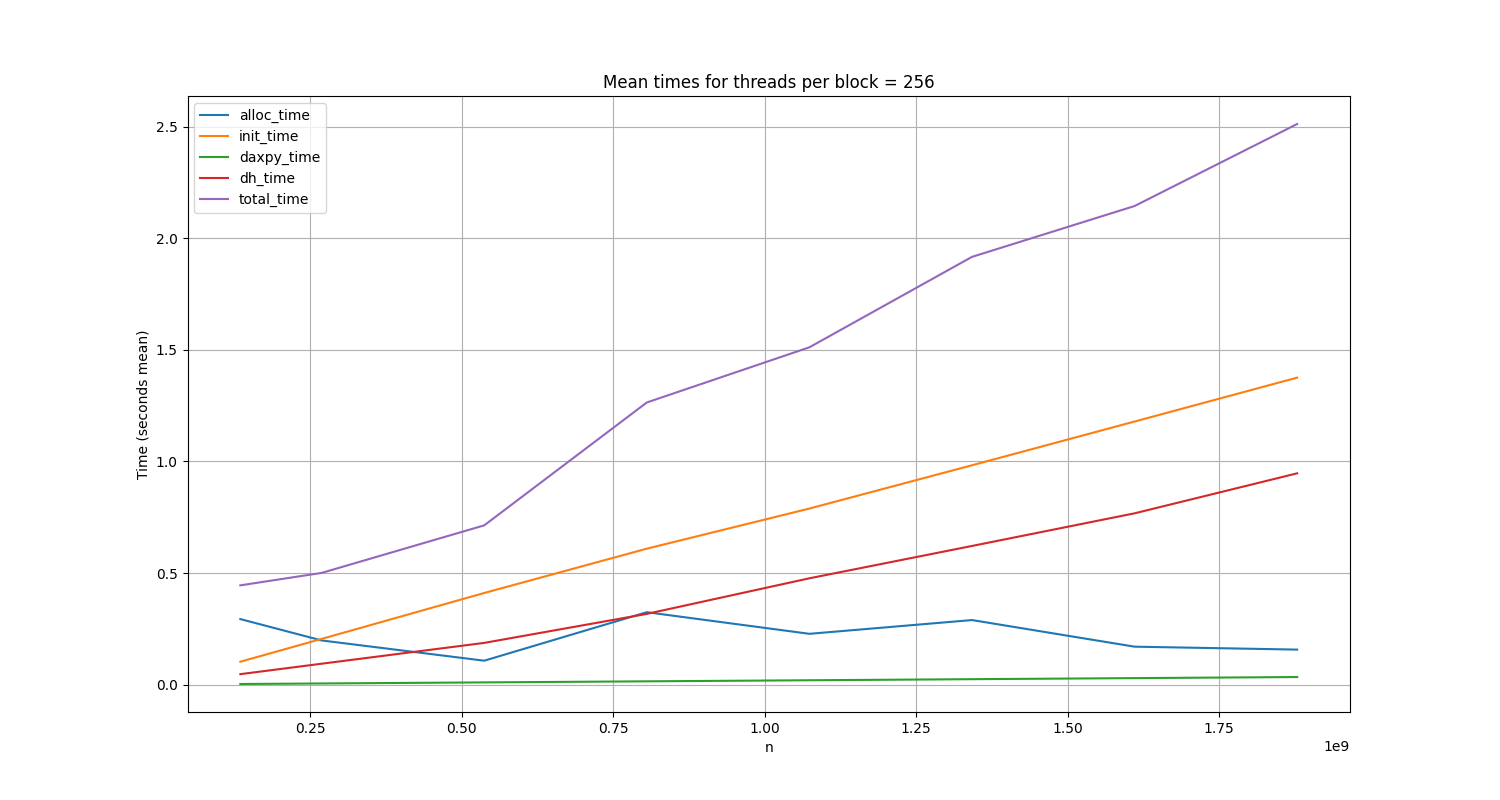
\includegraphics[width=0.9\textwidth]{images/daxpy/mean_times_256.png}
            }
            \caption{Mediciones de tiempo obtenidas para diferentes tamaños de problema.}
            \label{fig:daxpy_mean_times_256}
        \end{figure}        

        Un análisis pormenorizado de los componentes temporales revela características fundamentales del comportamiento de la implementación:
        
        \begin{itemize}
        
            \item El tiempo de inicialización (\texttt{init\_time}) domina el rendimiento global para problemas de gran magnitud, incrementando desde aproximadamente 0.1 segundos hasta 1.4 segundos a medida que aumenta el tamaño del problema. Este comportamiento se atribuye a la función \textit{kernel} \texttt{init\textless\textless\textless blocksPerGrid, threadsPerBlock\textgreater\textgreater\textgreater} que debe inicializar cada elemento de los vectores \texttt{x} e \texttt{y}. La clara progresión lineal confirma que la inicialización está limitada principalmente por el ancho de banda de memoria, no por la capacidad computacional intrínseca de la GPU.
            
            \item El tiempo de transferencia de datos hacia el host (\texttt{dh\_time}), implementado mediante \texttt{cudaMemPrefetchAsync}, exhibe asimismo un incremento lineal conforme aumenta el tamaño del problema. Este comportamiento es coherente con las expectativas teóricas, dado que el volumen de datos transferidos es directamente proporcional a $n$. La pendiente menos pronunciada en comparación con \texttt{init\_time} sugiere un aprovechamiento más eficiente del ancho de banda PCIe durante la transferencia unidireccional.
        
            \item El tiempo de asignación de memoria (\texttt{alloc\_time}) presenta un comportamiento particularmente interesante: inicialmente aumenta con el tamaño del problema hasta aproximadamente $n \approx 0.75 \times 10^9$, pero posteriormente se estabiliza e incluso manifiesta una ligera disminución. Este patrón no monotónico podría atribuirse a mecanismos internos de optimización en la gestión de memoria unificada de CUDA, como la asignación bajo demanda o la reserva anticipada de grandes bloques contiguos de memoria.
        
            \item El tiempo de ejecución específico del \textit{kernel} DAXPY (\texttt{daxpy\_time}) permanece notablemente constante y reducido (cercano a 0.05 segundos) independientemente del tamaño del problema. Este excepcional rendimiento se atribuye a dos factores fundamentales en la implementación:
        
                \begin{enumerate}
                
                    \item La utilización de un patrón de acceso con \textit{stride} en el \textit{kernel}. Esta estrategia permite que cada hilo procese múltiples elementos no contiguos, distribuyendo eficientemente la carga computacional incluso cuando el tamaño del problema excede significativamente el número total de hilos disponibles.
                    
                    \item La elevada intensidad aritmética característica de la operación DAXPY, combinada con un patrón de acceso a memoria perfectamente coalescente, maximiza la utilización efectiva del ancho de banda de memoria disponible en la GPU.
                    
                \end{enumerate}

        \end{itemize}
        
        La escalabilidad observada corrobora que la implementación está limitada principalmente por operaciones intensivas en memoria (inicialización y transferencia de datos), no por capacidad computacional, lo cual es característico de algoritmos clasificados como \textit{memory-bound}, como DAXPY, que presentan una relación operaciones aritméticas/accesos a memoria extremadamente baja.
        
    \subsection{Tiempo de ejecución}

        La figura \ref{fig:daxpy_times_per_threadsPerBlock} desglosa los tiempos de ejecución según la configuración de hilos por bloque, revelando patrones críticos para la optimización del rendimiento:

        \begin{figure}[H]
            \centering
            \fbox{
                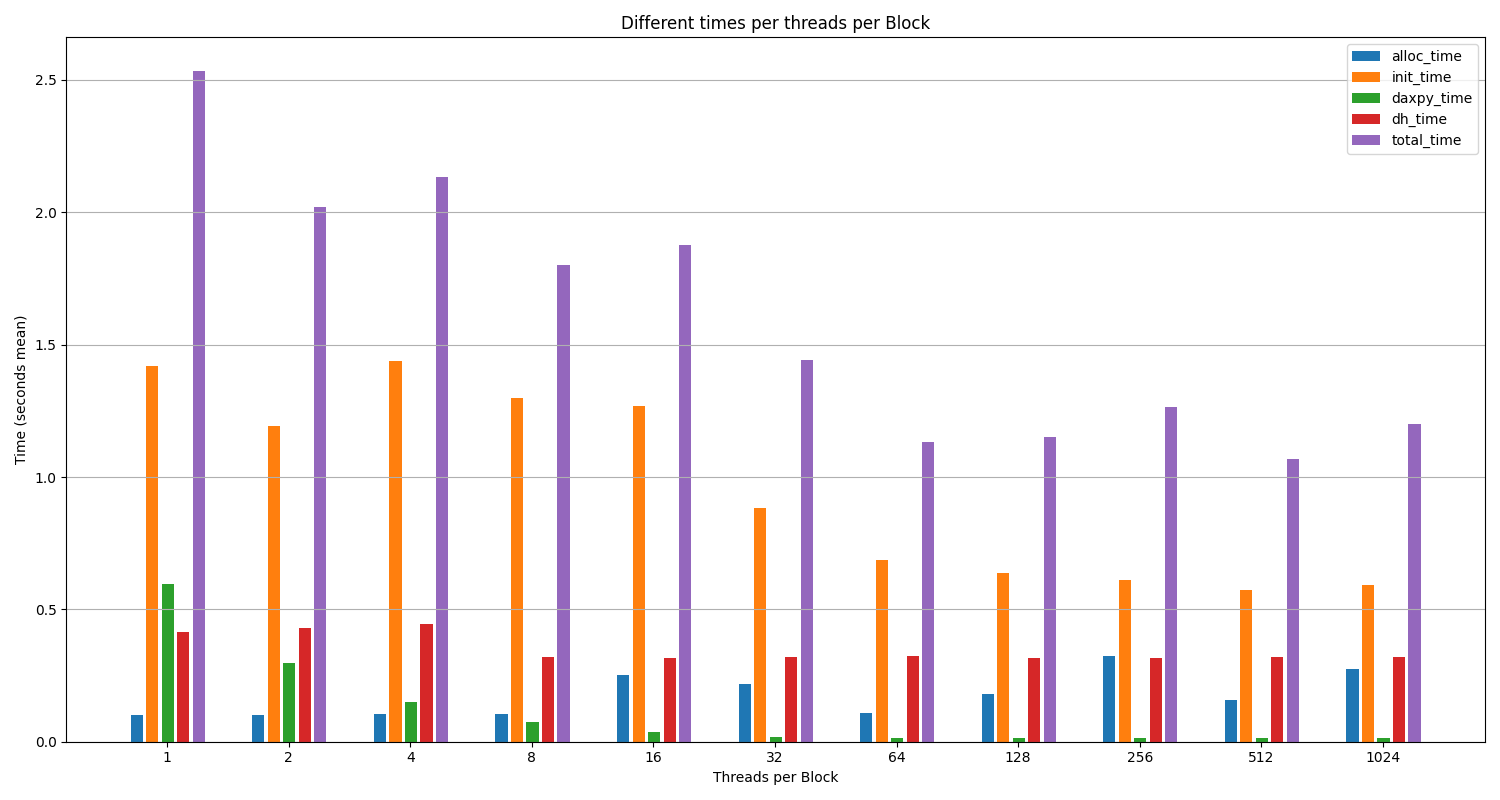
\includegraphics[width=0.9\textwidth]{images/daxpy/times_per_threadsPerBlock.png}
            }
            \caption{Mediciones de tiempo obtenidas para diferentes tamaños de bloques y \textit{grid}.}
            \label{fig:daxpy_times_per_threadsPerBlock}
        \end{figure}  
        
        \begin{itemize}
        
            \item Para configuraciones con baja densidad de hilos por bloque (1-4), el tiempo total de ejecución resulta excesivamente elevado (2.5 segundos para la configuración de 1 hilo por bloque). Este deficiente rendimiento se atribuye fundamentalmente a la incapacidad intrínseca de ocultar latencias de acceso a memoria y a la severa subutilización de los recursos computacionales disponibles en la GPU. Con tan escasa cantidad de hilos, la mayoría de los CUDA \textit{cores} permanecen en estado de inactividad, y el \textit{warp scheduler }no logra aprovechar eficientemente el paralelismo a nivel de \textit{warp} para mitigar las latencias de memoria.
            
            \item El tiempo de inicialización (\texttt{init\_time}) exhibe una pronunciada disminución al incrementar el número de hilos por bloque hasta aproximadamente 32 hilos, para luego continuar decreciendo más gradualmente. Este comportamiento se alinea perfectamente con la arquitectura de \textit{warps} característica de NVIDIA, donde cada \textit{warp} consta de exactamente 32 hilos ejecutándose en \textit{lockstep}. Las configuraciones por debajo de 32 hilos subutilizan inherentemente los recursos del \textit{warp} y generan un \textit{scheduling} ineficiente.
            
            \item El tiempo de ejecución específico del \textit{kernel} DAXPY (\texttt{daxpy\_time}) muestra una tendencia particularmente reveladora: es significativamente elevado (0.6 segundos) para la configuración de 1 hilo por bloque y disminuye rápidamente, tornándose prácticamente insignificante para configuraciones con más de 16 hilos por bloque. Esto evidencia la extraordinaria efectividad del paralelismo en la ocultación de latencias de memoria cuando se utiliza una cantidad suficiente de hilos, permitiendo que el \textit{kernel} opere a velocidades próximas al límite teórico impuesto por el ancho de banda de memoria.
            
            \item El punto óptimo de configuración se sitúa en torno a 128-256 hilos por bloque, donde el tiempo total alcanza su mínimo. Configuraciones con mayor densidad de hilos (512, 1024) no ofrecen mejoras adicionales significativas, lo que sugiere que otros factores limitantes, como la presión sobre los registros disponibles o la memoria compartida, podrían estar estableciendo un límite superior al rendimiento alcanzable.
        
        \end{itemize}
               
        El patrón de acceso implementado, conocido como ``grid-stride loop'', permite que la implementación escale eficientemente independientemente de la relación entre el tamaño del problema y el número total de hilos disponibles. Cuando se dispone de una cantidad insuficiente de hilos, cada hilo debe procesar secuencialmente numerosos elementos, lo que explica el deficiente rendimiento observado con configuraciones de baja densidad de hilos por bloque. Al incrementar el número de hilos, la carga computacional por hilo disminuye significativamente, mejorando la capacidad de ocultación de latencias y optimizando la utilización global de los recursos.
        
    \subsection{Ocupancia}

        La figura \ref{fig:daxpy_occupancy_per_threadsPerBlock} ilustra con precisión cómo la ocupancia teórica de los multiprocesadores de la GPU (SM) varía en función del número de hilos por bloque, proporcionando \textit{insights} fundamentales sobre la utilización de recursos:

        \begin{figure}[H]
            \centering
            \fbox{
                \includegraphics[width=0.9\textwidth]{images/daxpy/occupancy_per_threadsPerBlock.png}
            }
            \caption{Valores de ocupancia teorica para distintos valores de tamaño de bloque.}
            \label{fig:daxpy_occupancy_per_threadsPerBlock}
        \end{figure}  
        
        \begin{itemize}
        
            \item Para configuraciones con baja densidad de hilos por bloque (1-32), la ocupancia se mantiene en niveles extremadamente reducidos (inferior a 0.5), lo que explica satisfactoriamente el deficiente rendimiento observado en estas configuraciones. Cuando la ocupancia es baja, el \textit{hardware} no puede implementar eficazmente mecanismos para ocultar latencias de acceso a memoria mediante el cambio de contexto entre \textit{warps}, resultando en una ejecución notablemente ineficiente.
            
            \item Un punto de inflexión crítico se observa en la configuración de 64 hilos por bloque, donde la ocupancia alcanza súbitamente el valor máximo de 1.0 (100\%). Esta ocupancia óptima se mantiene constante para todas las configuraciones de mayor densidad (128, 256, 512, 1024 hilos por bloque). Este comportamiento se relaciona directamente con los algoritmos de cálculo de ocupancia implementados en el código. La ocupancia perfecta indica que la GPU logra mantener suficientes bloques activos por SM para saturar completamente sus recursos de ejecución, lo que teóricamente debería traducirse en un rendimiento óptimo.
            
            \item Resulta particularmente significativo observar que, a pesar de alcanzar una ocupancia perfecta a partir de 64 hilos por bloque, el rendimiento óptimo (figura 1) se manifiesta con configuraciones de 128-256 hilos por bloque. Esta aparente discrepancia revela que la ocupancia teórica no constituye el único factor determinante del rendimiento práctico. Otros factores críticos como el tamaño del \textit{working} set en las cachés L1/L2, la eficiencia en la coalescencia de accesos a memoria, y la potencial divergencia de \textit{warps} desempeñan roles igualmente importantes en la determinación del rendimiento global.
        
        \end{itemize}
        
        La ocupancia está influenciada principalmente por tres limitaciones fundamentales de recursos: el número de registros disponibles por hilo, la cantidad de memoria compartida por bloque y el número máximo de hilos que pueden residir simultáneamente en cada SM. En este caso particular, dado que el \textit{kernel} DAXPY presenta una estructura relativamente simple y utiliza una cantidad reducida de registros sin requerir memoria compartida, el factor limitante predominante es probablemente el número máximo de \textit{threads} que pueden coexistir simultáneamente en cada SM. A partir de cierto umbral (64 hilos por bloque), el \textit{hardware} logra programar eficientemente suficientes \textit{warps} para mantener todos los CUDA \textit{cores} en estado de ocupación incluso cuando algunos \textit{warps} se encuentran en espera por operaciones de memoria.

    \subsection{Matriz de isoeficiencia}

        La figura \ref{fig:daxpy_isoEfficiencyMatrix} presenta una matriz de isoeficiencia que proporciona una visión holística y multidimensional del rendimiento en función de dos variables críticas: el tamaño del problema (eje horizontal) y el número de hilos por bloque (eje vertical). Esta sofisticada visualización permite identificar regiones de eficiencia comparable a través de diversas configuraciones.

        \begin{figure}[H]
            \centering
            \fbox{
                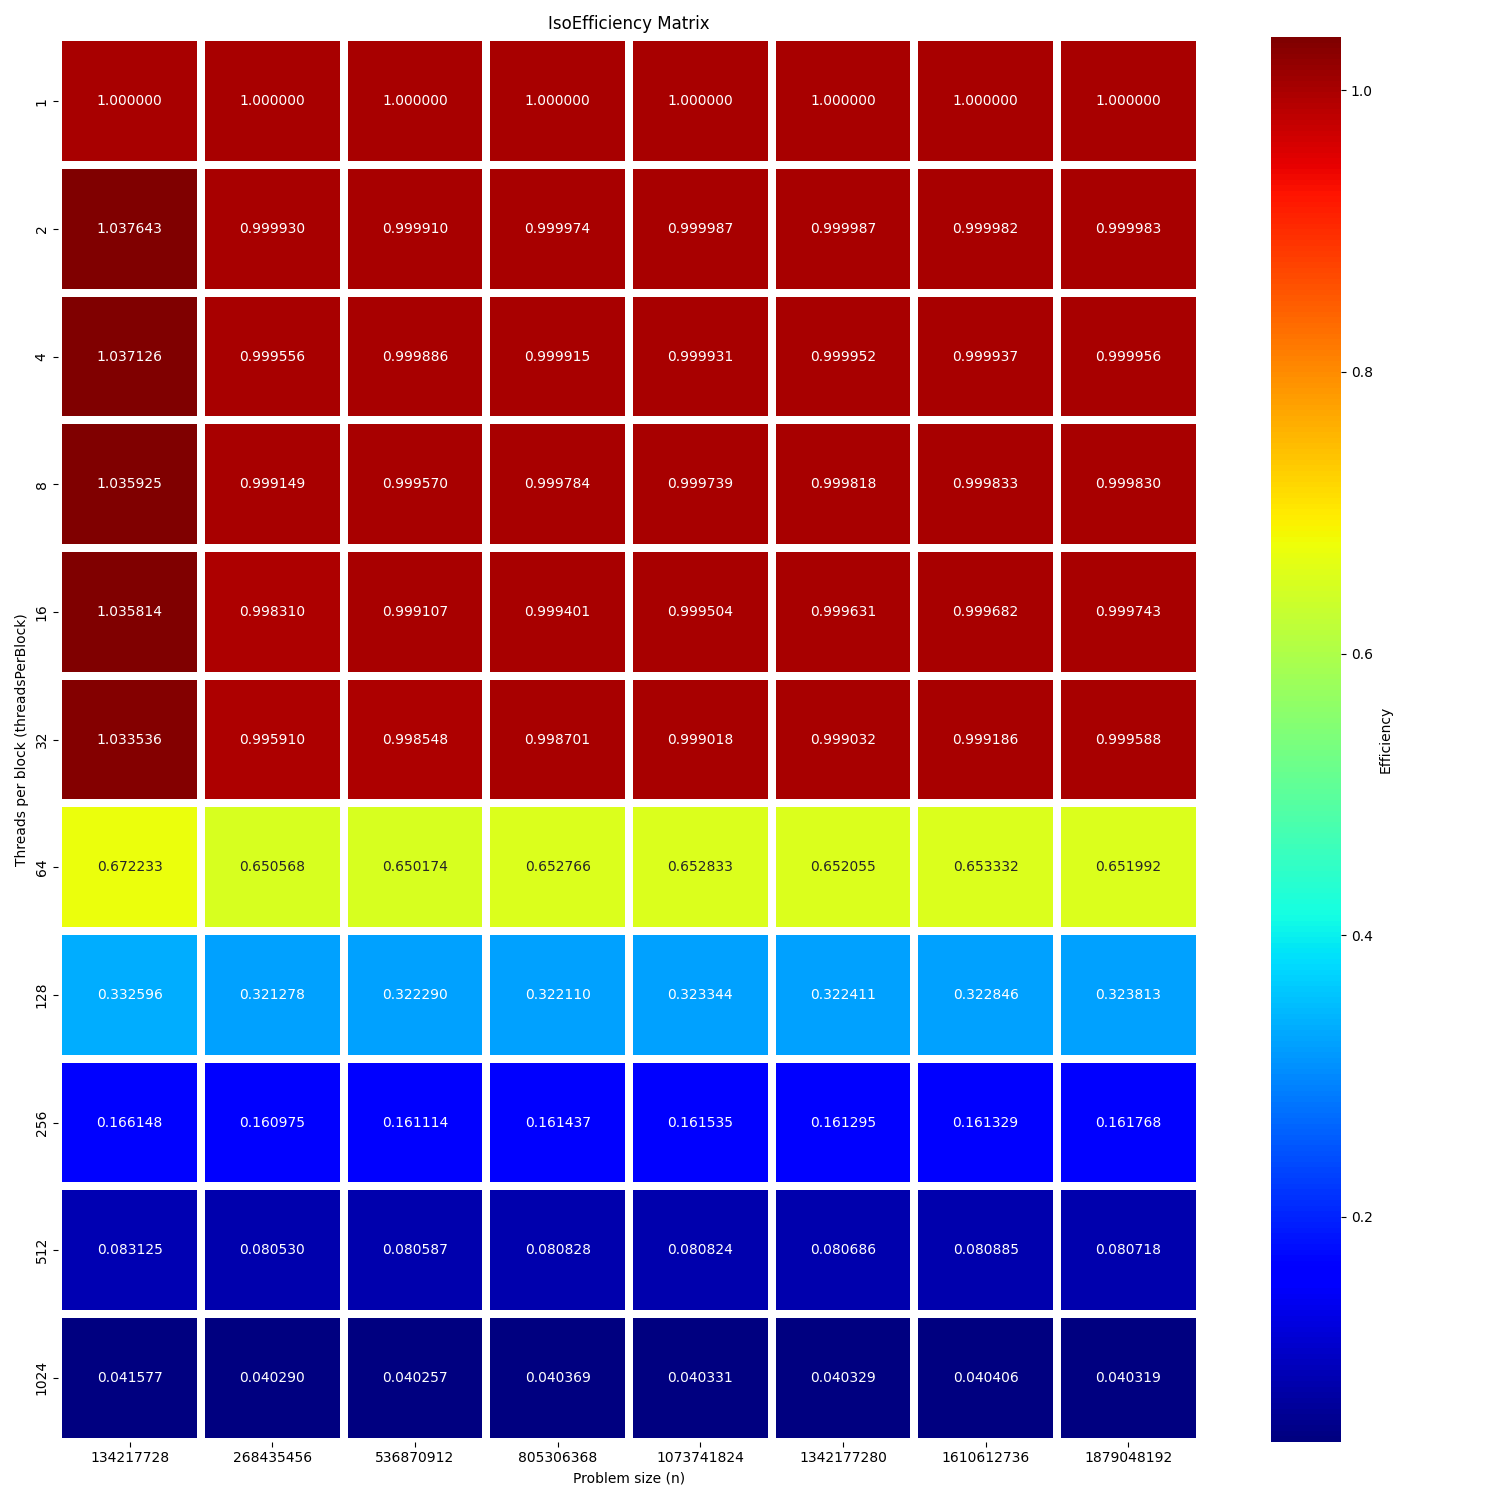
\includegraphics[width=0.9\textwidth]{images/daxpy/isoEfficiencyMatrix.png}
            }
            \caption{Matriz de isoeficiencia.}
            \label{fig:daxpy_isoEfficiencyMatrix}
        \end{figure}  
        
        \begin{itemize}
        
            \item Las configuraciones con baja densidad de hilos por bloque (1-32) exhiben una eficiencia aparentemente elevada (valores cercanos a 1.0), representada mediante tonalidades rojizas en la región superior de la matriz. Sin embargo, esta elevada eficiencia resulta engañosa cuando se analiza en conjunción con los resultados de tiempo de ejecución y ocupancia. Estas configuraciones son ``eficientes'' únicamente en el sentido de que mantienen una relación relativamente constante entre rendimiento y recursos utilizados, pero su rendimiento absoluto es marcadamente deficiente debido a la insuficiente utilización de los recursos computacionales disponibles en la GPU.
        
            \item Se observa una transición dramática en la eficiencia precisamente en la configuración de 64 hilos por bloque, donde los valores experimentan una súbita reducción hasta aproximadamente 0.67 (representada mediante tonalidades amarillentas). Esta transición crítica coincide exactamente con el punto donde la ocupancia alcanza su valor máximo de 1.0, lo que sugiere convincentemente que a partir de este umbral la implementación está limitada fundamentalmente por el ancho de banda de memoria disponible, no por la capacidad computacional intrínseca.
            
            \item Las configuraciones con alta densidad de hilos por bloque (128 o superior) muestran una eficiencia progresivamente decreciente (tonalidades azuladas), con valores que descienden hasta aproximadamente 0.04 para la configuración máxima de 1024 hilos por bloque. Esta disminución no debe interpretarse necesariamente como un deterioro del rendimiento absoluto, sino como una indicación de que estas configuraciones no escalan linealmente con el incremento de recursos asignados.
            
            \item Resulta particularmente notable que la eficiencia se mantiene notablemente constante a través de diferentes tamaños de problema para una configuración dada de hilos por bloque, como se evidencia por la uniformidad cromática en cada fila horizontal de la matriz. Esta observación corrobora que el rendimiento está determinado principalmente por el grado de paralelismo implementado (hilos por bloque) y no por el tamaño específico del problema, una vez que éste supera cierto umbral crítico.
            
        \end{itemize}
        
        La interpretación comprehensiva de esta matriz debe realizarse necesariamente en conjunción con las restantes métricas analizadas. Por ejemplo, aunque las configuraciones con baja densidad de hilos por bloque exhiben una elevada ``eficiencia'' aparente, sabemos por los análisis de ocupancia y tiempo de ejecución (Figuras 2 y 1, respectivamente) que su rendimiento absoluto es notablemente deficiente debido a la insuficiente ocupancia. La matriz resalta claramente que, para este algoritmo clasificado como \textit{memory-bound}, existe un punto óptimo en torno a 64-128 hilos por bloque que establece un equilibrio adecuado entre ocupancia efectiva y otros factores limitantes como la presión sobre los registros disponibles y las cachés.

        Esta sofisticada visualización refleja asimismo una característica fundamental de los algoritmos \textit{ memory-bound} como DAXPY: una vez que se alcanza un nivel suficiente de paralelismo para saturar completamente el ancho de banda de memoria disponible, la incorporación de paralelismo adicional no contribuye significativamente a la mejora del rendimiento, resultando en una eficiencia aparentemente reducida, pero manteniendo un rendimiento absoluto óptimo desde la perspectiva práctica.

    \subsection{Métricas generales}

        \begin{table}[H]
            \centering
            \begin{adjustbox}{width=\textwidth, keepaspectratio}
                \begin{tabular}{rrrrrrrrr}
                    \toprule
                    Threads & N & Max Time & Ref Time & Speedup & Efficiency & Quality & Secuential Compute Speedup & Secuential Total Speedup \\
                    \midrule
                    16 & 134217728 & 0.01 & 0.10 & 16.57 & 1.04 & 160.57 & 136.71 & 11.46 \\
                    32 & 134217728 & 0.00 & 0.10 & 33.07 & 1.03 & 320.43 & 272.81 & 5.59 \\
                    64 & 134217728 & 0.00 & 0.10 & 43.02 & 0.67 & 416.83 & 354.89 & 5.84 \\
                    128 & 134217728 & 0.00 & 0.10 & 42.57 & 0.33 & 412.46 & 351.17 & 5.95 \\
                    256 & 134217728 & 0.00 & 0.10 & 42.53 & 0.17 & 412.09 & 350.85 & 5.91 \\
                    512 & 134217728 & 0.00 & 0.10 & 42.56 & 0.08 & 412.34 & 351.07 & 5.52 \\
                    1024 & 134217728 & 0.00 & 0.10 & 42.58 & 0.04 & 412.49 & 351.19 & 5.99 \\
                    
                    16 & 268435456 & 0.01 & 0.20 & 15.97 & 1.00 & 80.32 & 68.39 & 4.89 \\
                    32 & 268435456 & 0.01 & 0.20 & 31.87 & 1.00 & 160.26 & 136.45 & 4.39 \\
                    64 & 268435456 & 0.00 & 0.20 & 41.64 & 0.65 & 209.38 & 178.26 & 4.79 \\
                    128 & 268435456 & 0.00 & 0.20 & 41.12 & 0.32 & 206.80 & 176.07 & 4.85 \\
                    256 & 268435456 & 0.00 & 0.20 & 41.21 & 0.16 & 207.23 & 176.44 & 4.92 \\
                    512 & 268435456 & 0.00 & 0.20 & 41.23 & 0.08 & 207.34 & 176.53 & 5.00 \\
                    1024 & 268435456 & 0.00 & 0.20 & 41.26 & 0.04 & 207.47 & 176.64 & 5.02 \\

                    16 & 536870912 & 0.02 & 0.40 & 15.99 & 1.00 & 40.20 & 34.22 & 2.29 \\
                    32 & 536870912 & 0.01 & 0.40 & 31.95 & 1.00 & 80.35 & 68.41 & 3.15 \\
                    64 & 536870912 & 0.01 & 0.40 & 41.61 & 0.65 & 104.63 & 89.08 & 5.58 \\
                    128 & 536870912 & 0.01 & 0.40 & 41.25 & 0.32 & 103.73 & 88.32 & 5.76 \\
                    256 & 536870912 & 0.01 & 0.40 & 41.25 & 0.16 & 103.71 & 88.30 & 5.98 \\
                    512 & 536870912 & 0.01 & 0.40 & 41.26 & 0.08 & 103.75 & 88.33 & 6.08 \\
                    1024 & 536870912 & 0.01 & 0.40 & 41.22 & 0.04 & 103.65 & 88.25 & 5.98 \\
                   
                    16 & 805306368 & 0.04 & 0.60 & 15.99 & 1.00 & 26.81 & 22.82 & 1.88 \\
                    32 & 805306368 & 0.02 & 0.60 & 31.96 & 1.00 & 53.57 & 45.61 & 2.30 \\
                    64 & 805306368 & 0.01 & 0.60 & 41.78 & 0.65 & 70.03 & 59.63 & 3.79 \\
                    128 & 805306368 & 0.01 & 0.60 & 41.23 & 0.32 & 69.11 & 58.84 & 3.27 \\
                    256 & 805306368 & 0.01 & 0.60 & 41.33 & 0.16 & 69.28 & 58.98 & 3.32 \\
                    512 & 805306368 & 0.01 & 0.60 & 41.38 & 0.08 & 69.37 & 59.06 & 3.37 \\
                    1024 & 805306368 & 0.01 & 0.60 & 41.34 & 0.04 & 69.30 & 59.00 & 3.37 \\
                   
                    16 & 1073741824 & 0.05 & 0.80 & 15.99 & 1.00 & 20.11 & 17.12 & 1.66 \\
                    32 & 1073741824 & 0.02 & 0.80 & 31.97 & 1.00 & 40.19 & 34.22 & 1.86 \\
                    64 & 1073741824 & 0.02 & 0.80 & 41.78 & 0.65 & 52.53 & 44.72 & 2.31 \\
                    128 & 1073741824 & 0.02 & 0.80 & 41.39 & 0.32 & 52.03 & 44.30 & 2.44 \\
                    256 & 1073741824 & 0.02 & 0.80 & 41.35 & 0.16 & 51.99 & 44.26 & 2.49 \\
                    512 & 1073741824 & 0.02 & 0.80 & 41.38 & 0.08 & 52.03 & 44.30 & 2.48 \\
                    1024 & 1073741824 & 0.02 & 0.80 & 41.30 & 0.04 & 51.92 & 44.21 & 2.49 \\
                    
                    16 & 1342177280 & 0.06 & 0.99 & 15.99 & 1.00 & 16.09 & 13.70 & 1.40 \\
                    32 & 1342177280 & 0.03 & 0.99 & 31.97 & 1.00 & 32.15 & 27.38 & 1.70 \\
                    64 & 1342177280 & 0.02 & 0.99 & 41.73 & 0.65 & 41.97 & 35.74 & 2.07 \\
                    128 & 1342177280 & 0.02 & 0.99 & 41.27 & 0.32 & 41.51 & 35.34 & 1.82 \\
                    256 & 1342177280 & 0.02 & 0.99 & 41.29 & 0.16 & 41.53 & 35.36 & 1.88 \\
                    512 & 1342177280 & 0.02 & 0.99 & 41.31 & 0.08 & 41.55 & 35.38 & 1.90 \\
                    1024 & 1342177280 & 0.02 & 0.99 & 41.30 & 0.04 & 41.54 & 35.36 & 1.87 \\
                    
                    16 & 1610612736 & 0.07 & 1.19 & 15.99 & 1.00 & 13.41 & 11.41 & 1.27 \\
                    32 & 1610612736 & 0.04 & 1.19 & 31.97 & 1.00 & 26.80 & 22.82 & 1.59 \\
                    64 & 1610612736 & 0.03 & 1.19 & 41.81 & 0.65 & 35.05 & 29.84 & 1.93 \\
                    128 & 1610612736 & 0.03 & 1.19 & 41.32 & 0.32 & 34.64 & 29.49 & 1.60 \\
                    256 & 1610612736 & 0.03 & 1.19 & 41.30 & 0.16 & 34.62 & 29.47 & 1.64 \\
                    512 & 1610612736 & 0.03 & 1.19 & 41.41 & 0.08 & 34.71 & 29.55 & 1.65 \\
                    1024 & 1610612736 & 0.03 & 1.19 & 41.38 & 0.04 & 34.68 & 29.53 & 1.61 \\
                   
                    16 & 1879048192 & 0.09 & 1.39 & 16.00 & 1.00 & 11.49 & 9.78 & 1.05 \\
                    32 & 1879048192 & 0.04 & 1.39 & 31.99 & 1.00 & 22.98 & 19.57 & 1.36 \\
                    64 & 1879048192 & 0.03 & 1.39 & 41.73 & 0.65 & 29.98 & 25.52 & 1.50 \\
                    128 & 1879048192 & 0.03 & 1.39 & 41.45 & 0.32 & 29.78 & 25.35 & 1.44 \\
                    256 & 1879048192 & 0.03 & 1.39 & 41.41 & 0.16 & 29.75 & 25.33 & 1.59 \\
                    512 & 1879048192 & 0.03 & 1.39 & 41.33 & 0.08 & 29.69 & 25.28 & 1.61 \\
                    1024 & 1879048192 & 0.03 & 1.39 & 41.29 & 0.04 & 29.66 & 25.25 & 1.58 \\
                    \bottomrule
                \end{tabular}
            \end{adjustbox}
            \caption{Métricas generales.}
            \label{tab:daxpy_metrics}
        \end{table}  

    \chapter{Ejercicio 3: Histograma}

\section{Introducción}

    El cálculo del histograma es una operación fundamental en el procesamiento de imágenes y el análisis de datos, que proporciona una representación visual de la distribución de la frecuencia de los valores dentro de un conjunto de datos. En el contexto del procesamiento de imágenes, un histograma típicamente ilustra la distribución de la intensidad de los píxeles, donde el eje horizontal representa los posibles valores de intensidad (por ejemplo, de 0 a 255 en imágenes de escala de grises) y el eje vertical representa el número de píxeles en la imagen que poseen esa intensidad. Para conjuntos de datos generales, un histograma puede representar la frecuencia de cualquier tipo de valor.
    
    Esta representación es crucial para una variedad de aplicaciones. En el procesamiento de imágenes, los histogramas se utilizan para técnicas como la ecualización de histogramas, que mejora el contraste de una imagen distribuyendo más uniformemente las intensidades de los píxeles. También son esenciales en la segmentación de imágenes, donde el análisis de los picos y valles en un histograma puede ayudar a identificar regiones de interés o separar objetos del fondo. Además, los histogramas juegan un papel importante en el reconocimiento de objetos, ya que las características del histograma de una región de una imagen pueden servir como descriptores para identificar objetos o patrones. En el análisis estadístico de datos, los histogramas permiten visualizar la distribución de los datos, identificar valores atípicos y comprender la dispersión y la tendencia central de los datos.
    
    El cálculo del histograma se caracteriza por su naturaleza inherentemente paralela, ya que el procesamiento de cada elemento de los datos (ya sea un píxel en una imagen o un punto de datos en un conjunto de datos) puede contribuir independientemente al conteo de su correspondiente ``bin'' o intervalo en el histograma. Esta independencia permite que el cálculo del histograma se beneficie enormemente de las arquitecturas de computación paralela, como las GPUs. Sin embargo, el cálculo del histograma también presenta desafíos significativos, especialmente en implementaciones paralelas. Uno de los principales desafíos es la gestión eficiente de la memoria, ya que el histograma en sí debe almacenarse y actualizarse de manera eficiente. Además, cuando múltiples hilos de ejecución intentan actualizar simultáneamente el conteo de un mismo \textit{bin}, pueden ocurrir condiciones de carrera, lo que requiere el uso de mecanismos de sincronización para garantizar la corrección de los resultados.
    
    Este apartado presenta dos implementaciones del algoritmo del histograma utilizando CUDA, una plataforma de computación paralela de NVIDIA: una implementación que utiliza memoria global y otra que utiliza memoria compartida. La memoria global es la memoria principal de la GPU, accesible por todos los hilos, pero con una latencia relativamente alta. La memoria compartida, por otro lado, es una memoria \textit{on-chip}, mucho más rápida que la memoria global, pero de menor tamaño y accesible solo por los hilos dentro de un mismo bloque. Se analizará exhaustivamente el rendimiento de ambas implementaciones en la GPU NVIDIA A100, disponible en el centro de supercomputación CESGA. Se examinará no solo el rendimiento bruto de las implementaciones, sino también aspectos críticos como la escalabilidad (cómo se comporta el rendimiento al aumentar el tamaño de los datos), la eficiencia de utilización de los recursos de la GPU (como los multiprocesadores y la memoria), y las compensaciones entre diferentes estrategias de gestión de memoria (memoria global vs. memoria compartida) para identificar las estrategias óptimas de implementación del cálculo del histograma en arquitecturas paralelas.

\newpage

\section{Fundamentos teóricos}

    \subsection{Algoritmo de cálculo de histogramas}

        El cálculo de histogramas es una operación fundamental en el procesamiento de imágenes y análisis de datos. Dado un conjunto de valores (en este caso, los píxeles de una imagen en escala de grises), el histograma cuenta la frecuencia de cada valor en un rango predefinido (por ejemplo, 0 a 255 para imágenes de 8 bits). Matemáticamente, el histograma se define como:

        \begin{align}
            H[i] = \sum_{j=0}^{N-1} \delta(I[j], i), \quad \text{para } i = 0, 1, \ldots, L-1
        \end{align}

        Donde:

        \begin{itemize}
        
            \item \( I \) es el vector de píxeles de la imagen.
            
            \item \( N \) es el número total de píxeles en la imagen.
            
            \item \( L \) es el número de niveles de gris (por ejemplo, 256 para imágenes de 8 bits).
            
            \item \( \delta(I[j], i) \) es una función delta que devuelve 1 si \( I[j] = i \) y 0 en caso contrario.
            
        \end{itemize}

        El cálculo del histograma es una operación que se puede paralelizar eficientemente en GPU, ya que cada píxel puede ser procesado de manera independiente. Sin embargo, la acumulación de los valores en el histograma requiere sincronización para evitar condiciones de carrera. Esto se debe a que múltiples hilos pueden intentar actualizar el mismo contador del histograma simultáneamente, lo que podría llevar a resultados incorrectos si no se maneja adecuadamente.

        \subsubsection{Propiedades del cálculo de histogramas}

            El cálculo de histogramas presenta las siguientes propiedades computacionales:
            
            \begin{itemize}
            
                \item \textbf{Independencia de datos}: Cada píxel puede ser procesado de manera independiente, lo que permite una paralelización perfecta. Sin embargo, la acumulación de los conteos en el histograma global requiere sincronización.
                
                \item \textbf{Intensidad aritmética baja}: El cálculo de histogramas es una operación \textit{memory-bound}, ya que implica más accesos a memoria que operaciones aritméticas. Cada píxel requiere una lectura de memoria y una actualización del contador correspondiente en el histograma.
               
                \item \textbf{Patrones de acceso irregulares}: A diferencia de algoritmos como DAXPY, donde los accesos a memoria son secuenciales, el cálculo de histogramas implica accesos aleatorios a los contadores del histograma, lo que puede generar contención en la memoria global.
                
            \end{itemize}

    \subsection{Memoria global en CUDA}

        La memoria global en CUDA es la memoria principal de la GPU, accesible por todos los hilos de todos los bloques. Es la memoria más grande disponible en la GPU, pero también es la más lenta en términos de latencia y ancho de banda en comparación con otros tipos de memoria como la memoria compartida o los registros. En el contexto del cálculo de histogramas, la memoria global se utiliza para almacenar la imagen de entrada y el histograma final.

        \subsubsection{Características de la memoria global}

            \begin{itemize}
               
                \item \textbf{Alto ancho de banda, alta latencia}: Aunque la memoria global tiene un ancho de banda considerable, su latencia es alta. Para mitigar esto, es crucial optimizar los patrones de acceso a memoria.
                
                \item \textbf{Acceso coalescente}: Para maximizar el rendimiento, los accesos a la memoria global deben ser coalescentes, es decir, los hilos dentro de un mismo \textit{warp} deben acceder a posiciones de memoria contiguas. Esto permite que el \textit{hardware} consolide múltiples accesos en una sola transacción de memoria.
               
                \item \textbf{Uso de operaciones atómicas}: En el cálculo de histogramas, la memoria global se utiliza para almacenar el histograma final. Dado que múltiples hilos pueden actualizar el mismo contador, es necesario utilizar operaciones atómicas para garantizar la coherencia. Sin embargo, el uso excesivo de operaciones atómicas puede generar contención y reducir el rendimiento.
                
            \end{itemize}
        
        \subsubsection{Optimización del acceso a la memoria global}
        
            Para optimizar el acceso a la memoria global en el cálculo de histogramas, se pueden aplicar las siguientes técnicas:
            
            \begin{itemize}
                
                \item \textbf{Coalescencia de accesos}: Asegurar que los hilos dentro de un mismo \textit{warp} accedan a posiciones de memoria contiguas. Esto se logra organizando los datos de manera que los hilos procesen elementos consecutivos del vector de entrada.
                
                \item \textbf{\textit{Prefetching}}: Anticipar los accesos a memoria para reducir la latencia. Esto se puede lograr utilizando técnicas como \texttt{cudaMemPrefetchAsync} para mover los datos a la GPU antes de que sean necesarios.
                
                \item \textbf{Reducción de la contención atómica}: Minimizar el uso de operaciones atómicas en la memoria global utilizando técnicas como la reducción paralela en memoria compartida antes de actualizar el histograma global.
          
            \end{itemize}

    \subsection{Memoria compartida en CUDA}

        La memoria compartida es un recurso crítico en CUDA para optimizar el rendimiento de algoritmos como el cálculo de histogramas. Es una memoria de alta velocidad que es accesible por todos los hilos dentro de un mismo bloque. Su uso permite reducir los accesos a la memoria global, que es más lenta, y mejorar el rendimiento general del \textit{kernel}.

        \subsubsection{Características de la memoria compartida}
        
            \begin{itemize}
                
                \item \textbf{Baja latencia}: La memoria compartida es mucho más rápida que la memoria global, con tiempos de acceso similares a los de los registros.
                
                \item \textbf{Acceso por bloque}: Cada bloque de hilos tiene su propia región de memoria compartida, que no es accesible por hilos de otros bloques.
                
                \item \textbf{Limitada en tamaño}: La memoria compartida es un recurso limitado. En la mayoría de las GPU modernas, cada bloque puede utilizar hasta 48 KB de memoria compartida. Esto significa que su uso debe ser cuidadosamente planificado para evitar agotar este recurso.
          
            \end{itemize}
        
        \subsubsection{Uso de la memoria compartida}
        
            En el cálculo de histogramas, la memoria compartida se utiliza para acumular los conteos parciales de cada bloque antes de combinarlos en el histograma global. Esto reduce la contención en la memoria global y mejora el rendimiento. La estrategia típica es:
            
            \begin{enumerate}
            
                \item Cada bloque de hilos calcula un histograma parcial en memoria compartida.
                
                \item Los histogramas parciales se combinan en el histograma global utilizando operaciones atómicas para garantizar la coherencia.
                
            \end{enumerate}
        
        \subsubsection{Optimización usando memoria compartida}
        
            Para optimizar el uso de la memoria compartida en el cálculo de histogramas, se pueden aplicar las siguientes técnicas:
            
            \begin{itemize}
            
                \item \textbf{Reducción de la contención}: Dividir el histograma en múltiples bancos para reducir la contención en los accesos a memoria compartida. Esto es especialmente útil cuando múltiples hilos intentan actualizar el mismo contador.
                
                \item \textbf{Uso eficiente del espacio}: Asegurar que la memoria compartida se utilice de manera eficiente, evitando el desperdicio de espacio. Por ejemplo, en el cálculo de histogramas, se puede utilizar un \textit{array} de tamaño fijo (256 elementos para imágenes de 8 bits) para almacenar los conteos parciales.
              
                \item \textbf{Sincronización entre hilos}: Utilizar \texttt{\_\_syncthreads()} para garantizar que todos los hilos dentro de un bloque hayan terminado de actualizar el histograma parcial antes de combinarlo en el histograma global.
            
            \end{itemize}

    \subsection{Configuración de bloques e hilos}
    
        La organización de los hilos en bloques y \textit{grids} es crucial para el rendimiento del cálculo de histogramas en CUDA. La configuración óptima depende del tamaño de la imagen y de las características del \textit{hardware}. En general, se busca maximizar la ocupación de los multiprocesadores (SMs) de la GPU, lo que se logra equilibrando el número de hilos por bloque y el número de bloques por \textit{grid}.
        
        \begin{lstlisting}[language=C, caption={Calculo de dimensiones de bloques y \textit{grid}.}, gobble=12]
            int threadsPerBlock = atoi(argv[2]);
            long blocksPerGrid = ceil(imageSize / threadsPerBlock);
        \end{lstlisting}
                
        Donde:
        
        \begin{itemize}
        
            \item \texttt{threadsPerBlock} es el número de hilos por bloque.
            
            \item \texttt{blocksPerGrid} es el número de bloques necesarios para cubrir todos los píxeles de la imagen.
            
        \end{itemize}

        \subsubsection{Consideraciones arquitectónicas}
        
            \begin{itemize}
            
                \item \textbf{Granularidad de los bloques}: El número de hilos por bloque determina la unidad básica de trabajo que se asigna a cada SM. Bloques más grandes pueden maximizar la utilización de recursos, pero podrían limitar el número de bloques concurrentes por SM.
                
                \item \textbf{Eficiencia de \textit{warps}}: Dado que los \textit{warps} son unidades de 32 hilos, tamaños de bloque que no sean múltiplos exactos de 32 resultarán en \textit{warps} parcialmente ocupados, desperdiciando capacidad computacional.
                
                \item \textbf{Balanceo de carga}: Un número suficientemente grande de bloques asegura que todos los SMs disponibles reciban trabajo, maximizando la utilización global de la GPU.
                
            \end{itemize}
        
    \subsection{Patrones de acceso a memoria}

        El rendimiento del cálculo de histogramas en GPU está fuertemente influenciado por los patrones de acceso a memoria. Para maximizar la eficiencia, es importante garantizar que los accesos a memoria global sean coalescentes, es decir, que los hilos dentro de un mismo \textit{warp} accedan a posiciones de memoria contiguas. Esto permite que el \textit{hardware} consolide múltiples accesos en una sola transacción de memoria.
        
        \subsubsection{Coalescencia de accesos}

            La coalescencia de accesos es fundamental para maximizar el rendimiento en arquitecturas GPU. Cuando los hilos dentro de un mismo \textit{warp} acceden a posiciones de memoria contiguas, el \textit{hardware} puede consolidar estos accesos en un número mínimo de transacciones de memoria, aprovechando al máximo el ancho de banda disponible.

        \subsubsection{Distribución cíclica mediante \textit{stride}}

            La utilización de un \textit{stride} igual al número total de hilos distribuye el trabajo cíclicamente entre todos los hilos disponibles. Esta estrategia presenta ventajas arquitectónicas significativas, como el balanceo de carga intrínseco y la amortización del \textit{overhead} de lanzamiento.

    \subsection{Análisis de ocupancia y rendimiento}

        La ocupancia es una métrica clave en CUDA que mide la proporción de recursos computacionales que están siendo utilizados activamente en comparación con el máximo teórico. Para el cálculo de histogramas, una alta ocupancia no siempre se traduce en un mejor rendimiento, ya que el algoritmo está limitado por el ancho de banda de memoria.
        
        \subsubsection{Cálculo de la ocupancia}

            La ocupancia se calcula utilizando la API de CUDA:
            
            \begin{lstlisting}[language=C, caption={Calculo de ocupancia teorica.}, gobble=16]
                int maxBlocksPerSM;
                cudaOccupancyMaxActiveBlocksPerMultiprocessor(&maxBlocksPerSM, histogram, threadsPerBlock, 0);
                float occupancy = (float)(maxBlocksPerSM * threadsPerBlock) / prop.maxThreadsPerMultiProcessor;
            \end{lstlisting}
            
            Donde:
            
            \begin{itemize}
            
                \item \texttt{maxBlocksPerSM} es el número máximo de bloques que pueden alocarse y ejecutarse simultáneamente en un multiprocesador de NVIDIA.

                \item \texttt{threadsPerBlock} es el número de hilos por bloque.

                \item \texttt{prop.maxThreadsPerMultiProcessor} es el número máximo de hilos que un multiprocesador puede manejar.
                
            \end{itemize}

    \subsection{Limitaciones y optimizaciones}

        A pesar de las optimizaciones, el cálculo de histogramas en GPU tiene limitaciones inherentes debido a la naturaleza del algoritmo. Algunas de estas limitaciones incluyen:
        
        \begin{itemize}
        
            \item \textbf{Contención en operaciones atómicas}: La acumulación de los conteos en el histograma global requiere el uso de operaciones atómicas, lo que puede generar contención y reducir el rendimiento.
            
            \item \textbf{Uso de memoria compartida}: La memoria compartida es un recurso limitado, y su uso excesivo puede reducir el número de bloques que se pueden ejecutar simultáneamente.
            
            \item \textbf{Ancho de banda de memoria}: El algoritmo está limitado por el ancho de banda de memoria, especialmente en imágenes grandes.
            
        \end{itemize}

        \subsubsection{Optimizaciones potenciales}
    
            Algunas optimizaciones potenciales incluyen:
            
            \begin{itemize}
            
                \item \textbf{Reducción de la contención atómica}: Utilizar técnicas como la reducción paralela para combinar los histogramas parciales antes de realizar operaciones atómicas en el histograma global.
                
                \item \textbf{Uso eficiente de la memoria compartida}: Optimizar el uso de la memoria compartida para maximizar la ocupación y reducir la contención.
                
                \item \textbf{\textit{Prefetching} de datos}: Anticipar los accesos a memoria para reducir la latencia.
                
            \end{itemize}
    
            Estas optimizaciones pueden mejorar significativamente el rendimiento del cálculo de histogramas en GPU, especialmente en aplicaciones de procesamiento de imágenes a gran escala.

\newpage

\section{Implementación}

    El cálculo de histogramas es una operación fundamental en el procesamiento de imágenes y análisis de datos, que consiste en contar la frecuencia de ocurrencia de cada valor en un conjunto de datos. En este caso, se ha implementado en CUDA utilizando dos enfoques distintos: uno que utiliza memoria global y otro que aprovecha la memoria compartida para optimizar el rendimiento. A continuación, se presenta un análisis detallado de ambas implementaciones, examinando las decisiones de diseño, las implicaciones arquitectónicas y las diferencias clave entre los dos enfoques.

    \subsection{Estructura general}
    
        Ambas implementaciones siguen una estructura modular que facilita la comprensión, el mantenimiento y la optimización del código. Los componentes principales incluyen:
        
        \begin{enumerate}
        
            \item \textbf{Funciones de utilidad}: Incluyen mecanismos para la medición precisa de tiempos utilizando \texttt{CLOCK\_MONOTONIC}, que proporciona una resolución de nanosegundos y es inmune a ajustes del sistema. Además, se incluyen rutinas de comprobación de errores que verifican las llamadas a la API de CUDA, garantizando la integridad de la ejecución y facilitando la depuración.
            
            \item \textbf{\textit{Kernel} de histograma}: El núcleo computacional del programa, implementa el cálculo del histograma de forma paralela. En una versión se utiliza memoria global, mientras que en la otra se aprovecha la memoria compartida para optimizar el rendimiento.
            
            \item \textbf{Implementación secuencial en CPU}: Una versión optimizada para CPU que sirve tanto para la verificación de resultados como para establecer una referencia de rendimiento. Esta implementación es esencial para garantizar la corrección de los resultados obtenidos en la GPU.
            
            \item \textbf{Función principal}: Coordina la ejecución de los diferentes componentes, gestiona la configuración de los parámetros de ejecución (como el número de \textit{threads} por bloque) y realiza mediciones detalladas de rendimiento. Además, se encarga de la asignación y liberación de memoria tanto en la CPU como en la GPU.
            
        \end{enumerate}

        Esta estructura no solo facilita la comprensión del código, sino que también permite aislar y medir con precisión el rendimiento de cada componente del sistema, identificando posibles cuellos de botella y oportunidades de optimización.

    \subsection{Gestión de memoria}

        La gestión de memoria es un aspecto crítico en el rendimiento de aplicaciones CUDA, especialmente en operaciones como el cálculo de histogramas, donde se realizan numerosos accesos a memoria. Ambas implementaciones utilizan la API de CUDA para asignar y transferir datos entre la CPU y la GPU, pero difieren en cómo manejan la memoria dentro del \textit{kernel}.
        
        \subsubsection{Memoria global en \texttt{histogram\_1.cu}}

            En la primera implementación (\texttt{histogram\_1.cu}), el \textit{kernel} utiliza memoria global para almacenar el histograma local de cada \textit{thread}. Esto implica que cada \textit{thread} accede directamente a la memoria global para actualizar el histograma, lo que puede resultar en un alto número de accesos a memoria y posibles contenciones en las operaciones atómicas.
            
            \begin{itemize}
            
                \item \textbf{Histograma local por \textit{thread}}: Cada \textit{thread} mantiene su propio histograma local en un \textit{array} en memoria global. Esto permite que los \textit{threads} trabajen de forma independiente, pero también implica que cada \textit{thread} debe realizar múltiples accesos a la memoria global, lo que puede ser costoso en términos de rendimiento.
                
                \item \textbf{Acceso coalescente}: Los \textit{threads} acceden a posiciones de memoria contiguas en el \textit{array} de entrada, lo que maximiza la eficiencia de las transacciones de memoria. Sin embargo, los accesos al histograma global no son coalescentes, ya que los \textit{threads} pueden actualizar \textit{bins} diferentes de forma aleatoria.
                
                \item \textbf{Actualización atómica}: Los \textit{threads} utilizan operaciones atómicas para actualizar el histograma global, lo que garantiza la corrección en presencia de múltiples \textit{threads} que actualizan el mismo \textit{bin}. Sin embargo, las operaciones atómicas pueden generar contención y reducir el rendimiento, especialmente cuando muchos \textit{threads} intentan actualizar el mismo \textit{bin} simultáneamente.
                
            \end{itemize}
                    
        \subsubsection{Memoria compartida en \texttt{histogram\_2.cu}}
        
            En la segunda implementación (\texttt{histogram\_2.cu}), el \textit{kernel} utiliza memoria compartida para almacenar un histograma local por bloque. Esto reduce el número de accesos a la memoria global y mejora la eficiencia al permitir que los \textit{threads} dentro de un bloque colaboren en la construcción del histograma antes de realizar una única actualización atómica en la memoria global.
        
            \begin{itemize}
            
                \item \textbf{Histograma local por bloque}: Cada bloque mantiene un histograma local en memoria compartida, lo que reduce el número de accesos a la memoria global. La memoria compartida es mucho más rápida que la memoria global, lo que permite a los \textit{threads} actualizar el histograma local de forma eficiente.
                
                \item \textbf{Inicialización de memoria compartida}: Los \textit{threads} dentro de un bloque inicializan el histograma compartido en paralelo, lo que mejora la eficiencia. Cada \textit{thread} es responsable de inicializar una porción del histograma compartido, lo que permite una distribución uniforme del trabajo.
                
                \item \textbf{Actualización atómica en memoria compartida}: Los \textit{threads} utilizan operaciones atómicas para actualizar el histograma compartido, lo que garantiza la corrección en presencia de múltiples \textit{threads} dentro del mismo bloque. Aunque las operaciones atómicas en memoria compartida también pueden generar contención, esta contención es limitada a los \textit{threads} dentro del mismo bloque, lo que reduce su impacto en el rendimiento global.
                
                \item \textbf{Actualización atómica en memoria global}: Una vez que el histograma compartido está completo, los \textit{threads} actualizan el histograma global utilizando operaciones atómicas. Esta actualización se realiza de forma más eficiente, ya que cada bloque realiza una única actualización atómica por \textit{bin} en lugar de múltiples actualizaciones atómicas por \textit{thread}.
                
            \end{itemize}
            
    \subsection{\textit{Kernel} con memoria global}
        
        El \textit{kernel} en \texttt{histogram\_1.cu} utiliza memoria global para almacenar el histograma local de cada \textit{thread}. A continuación, se presenta un análisis detallado de su implementación:
        
        \begin{lstlisting}[language=C, caption={\textit{Kernel} usando memoria global.}, gobble=12]
            __global__ void histogram(unsigned char* input, int* histogram, size_t imageSize) {
                unsigned int localHistogram[GRAY_LEVELS] = {0};
            
                int tid = blockIdx.x * blockDim.x + threadIdx.x;
                int stride = blockDim.x * gridDim.x;
            
                for (int i = tid; i < imageSize; i += stride) {
                    localHistogram[input[i]]++;
                }
            
                for (int binIdx = 0; binIdx < GRAY_LEVELS; binIdx++) {
                    if (localHistogram[binIdx] > 0) {
                        atomicAdd(&histogram[binIdx], localHistogram[binIdx]);
                    }
                }
            }
        \end{lstlisting}

        \subsubsection{Análisis del \textit{kernel}}

            \begin{itemize}
            
                \item \textbf{Paralelismo}: Cada \textit{thread} procesa una porción del \textit{array} de entrada, lo que permite una distribución uniforme del trabajo. El uso de un bucle con \texttt{stride} garantiza que todos los \textit{threads} contribuyan al cálculo del histograma, incluso cuando el número de \textit{threads} es menor que el tamaño del \textit{array} de entrada.
                
                \item \textbf{Histograma local}: Cada \textit{thread} mantiene su propio histograma local en un \textit{array} en memoria global. Esto permite que los \textit{threads} trabajen de forma independiente, pero también implica que cada \textit{thread} debe realizar múltiples accesos a la memoria global, lo que puede ser costoso en términos de rendimiento.
                
                \item \textbf{Actualización atómica}: Los \textit{threads} utilizan operaciones atómicas para actualizar el histograma global, lo que garantiza la corrección en presencia de múltiples \textit{threads} que actualizan el mismo \textit{bin}. Sin embargo, las operaciones atómicas pueden generar contención y reducir el rendimiento, especialmente cuando muchos \textit{threads} intentan actualizar el mismo \textit{bin} simultáneamente.
                
            \end{itemize}

    \subsection{\textit{Kernel} con memoria compartida}

        El \textit{kernel} en \texttt{histogram\_2.cu} utiliza memoria compartida para almacenar un histograma local por bloque. A continuación, se presenta un análisis detallado de su implementación:
        
        \begin{lstlisting}[language=C, caption={\textit{Kernel} usando memoria compartida.}, gobble=12]
            __global__ void histogram(unsigned char* input, int* globalHistogram, size_t imageSize) {
                __shared__ unsigned int sharedHistogram[GRAY_LEVELS];
            
                int tid = blockIdx.x * blockDim.x + threadIdx.x;
                int stride = blockDim.x * gridDim.x;
                int localThreadID = threadIdx.x;
            
                for (int i = localThreadID; i < GRAY_LEVELS; i += blockDim.x) {
                    sharedHistogram[i] = 0;
                }
            
                __syncthreads();
            
                for (int i = tid; i < imageSize; i += stride) {
                    unsigned char pixelValue = input[i];
                    atomicAdd(&sharedHistogram[pixelValue], 1);
                }
            
                __syncthreads();
            
                for (int i = localThreadID; i < GRAY_LEVELS; i += blockDim.x) {
                    if (sharedHistogram[i] > 0) {
                        atomicAdd(&globalHistogram[i], sharedHistogram[i]);
                    }
                }
            }
        \end{lstlisting}
        
        \subsubsection{Análisis del \textit{kernel}}
                        
            \begin{itemize}

                \item \textbf{Inicialización del histograma compartido}:  Cada \textit{thread} dentro de un bloque es responsable de inicializar una porción del histograma compartido. Esto se realiza en paralelo, lo que permite una distribución uniforme del trabajo. La inicialización se divide entre los \textit{threads} del bloque, donde cada \textit{thread} inicializa un subconjunto de los \textit{bins} del histograma. Esto es más eficiente que asignar la inicialización a un solo \textit{thread}, ya que se aprovecha el paralelismo dentro del bloque.
                
                \item \textbf{Uso de \texttt{\_\_syncthreads()}}: Después de la inicialización del histograma compartido, se llama a `\_\_syncthreads()`. Esta función es una barrera de sincronización que garantiza que todos los \textit{threads} dentro del bloque hayan completado la inicialización antes de que cualquier \textit{thread} proceda a la siguiente fase del cálculo. Esto es crucial para evitar condiciones de carrera, donde un \textit{thread} podría intentar leer o escribir en el histograma compartido antes de que otro \textit{thread} haya terminado de inicializarlo.
                
                \item \textbf{Cálculo del histograma local en memoria compartida}: Una vez que el histograma compartido está inicializado, los \textit{threads} comienzan a procesar el \textit{array} de entrada. Cada \textit{thread} procesa una porción del \textit{array} de entrada y actualiza el histograma compartido utilizando operaciones atómicas (\texttt{atomicAdd}). Estas operaciones atómicas garantizan que las actualizaciones al histograma compartido sean correctas incluso cuando múltiples \textit{threads} intentan actualizar el mismo \textit{bin} simultáneamente. Sin embargo, dado que la memoria compartida es mucho más rápida que la memoria global, la contención en las operaciones atómicas es menos costosa en términos de rendimiento.
                
                \item \textbf{Sincronización antes de la actualización global}: Después de que todos los \textit{threads} hayan terminado de procesar el \textit{array} de entrada y actualizar el histograma compartido, se llama nuevamente a \texttt{\_\_syncthreads()}. Esta segunda sincronización garantiza que todos los \textit{threads} dentro del bloque hayan completado sus contribuciones al histograma compartido antes de que cualquier \textit{thread} proceda a actualizar el histograma global. Esto es esencial para evitar que un \textit{thread} comience a actualizar el histograma global mientras otros \textit{threads} aún están procesando el \textit{array} de entrada.
                
                \item \textbf{Actualización del histograma global}: Finalmente, los \textit{threads} actualizan el histograma global utilizando operaciones atómicas. Cada \textit{thread} es responsable de actualizar una porción del histograma global, lo que permite una distribución uniforme del trabajo. La actualización se realiza de forma más eficiente que en la implementación que utiliza memoria global, ya que cada bloque realiza una única actualización atómica por \textit{bin} en lugar de múltiples actualizaciones atómicas por \textit{thread}.
                
            \end{itemize}
            
    \subsection{Configuración de ejecución}
    
        La configuración de ejecución en ambas implementaciones se determina dinámicamente según los parámetros de entrada:
        
        \begin{lstlisting}[language=C, caption={Calculo de las dimensiones del \textit{grid}.}, gobble=12]
            long blocksPerGrid = ceil(imageSize / threadsPerBlock);
        \end{lstlisting}
        
        Esta configuración permite explorar diferentes configuraciones de ejecución sin modificar el código fuente, facilitando la búsqueda de parámetros óptimos para cada combinación específica de hardware y tamaño de problema.
        
    \subsection{Medición de tiempos}
    
        Ambas implementaciones utilizan una función de alta precisión basada en el uso de \texttt{clock\_gettime} para medir el tiempo de cada fase crítica de la ejecución:
        
        \begin{lstlisting}[language=C, caption={Función de medición de tiempo.}, gobble=12]
            double get_time() {
                struct timespec ts;
                clock_gettime(CLOCK_MONOTONIC, &ts);
                return ts.tv_sec + ts.tv_nsec / 1.0e9;
            }
        \end{lstlisting}
    
        El programa mide meticulosamente el tiempo de cada fase crítica de la ejecución, incluyendo la asignación de memoria, la inicialización, la ejecución del \textit{kernel} y la transferencia de datos.
        
    \subsection{Verificación de resultados}
        
        Ambas implementaciones incluyen un mecanismo exhaustivo de verificación que compara los resultados obtenidos en la GPU con una implementación de referencia en CPU:
        
        \begin{lstlisting}[language=C, caption={Comprobación de errores.}, gobble=12]
            int errors = 0;
            for (int i = 0; i < GRAY_LEVELS; i++) {
                if (h_hist[i] != h_hist_cpu[i]) {
                    errors = 1;
                    break;
                }
            }
        \end{lstlisting}
        
        Este proceso de verificación garantiza la corrección de los resultados y proporciona información valiosa sobre la precisión de la implementación en GPU.

\newpage

\section{Resultados y análisis}
    
    \subsection{Introducción}

        En este apartado se analizan los resultados obtenidos en la implementación de algoritmos de histograma en GPU utilizando CUDA. Este análisis se centra en comparar dos implementaciones diferentes para el cálculo de histogramas: una basada en memoria global y otra que utiliza memoria compartida. Los histogramas son estructuras de datos fundamentales en el procesamiento de imágenes, que contabilizan la frecuencia de cada nivel de gris en una imagen.
        La implementación se ha realizado mediante dos \textit{kernels} CUDA distintos que procesan imágenes en formato PGM. El primer \textit{kernel} (\texttt{histogram\_1.cu}) utiliza exclusivamente memoria global con optimizaciones básicas como el uso de histogramas locales por \textit{thread} para reducir colisiones en los accesos atómicos. El segundo \textit{kernel} (\texttt{histogram\_2.cu}) implementa una versión más sofisticada que aprovecha la memoria compartida disponible en cada bloque de \textit{threads}, lo que potencialmente reduce la latencia de acceso a memoria y mejora el paralelismo.

        Para cada implementación, se ha medido el tiempo de ejecución dividido en diferentes fases: asignación de memoria (\texttt{alloc\_time}), inicialización (\texttt{init\_time}), cálculo del histograma (\texttt{histogram\_time}), transferencia de datos \textit{host-device} (\texttt{hd\_time}) y \textit{ device-host} (\texttt{dh\_time}). Adicionalmente, se calcula el tiempo total como la suma de todas estas fases. Las mediciones se han realizado variando el número de \textit{threads} por bloque (1, 2, 4, 8, 16, 32, 64, 128, 256, 512 y 1024) para estudiar su impacto en el rendimiento.

    \subsection{Escalabilidad}
    
        Las figuras \ref{fig:histogram_execution_times_global} y \ref{fig:histogram_execution_times_shared} presentan una evaluación cuantitativa del rendimiento de dos implementaciones algorítmicas divergentes para el cálculo de histogramas mediante CUDA: la primera basada en memoria global con reducción por thread y la segunda optimizada con memoria compartida utilizando reducción jerárquica por bloque. Ambas implementaciones fueron sometidas a evaluación utilizando un conjunto de imágenes de prueba con patrones estructurales específicos: gradientes por columnas, diagonal y filas, permitiendo analizar el impacto de la localidad espacial y los patrones de coherencia en acceso a datos.
        
        \begin{figure}[H]
            \centering
            \fbox{
                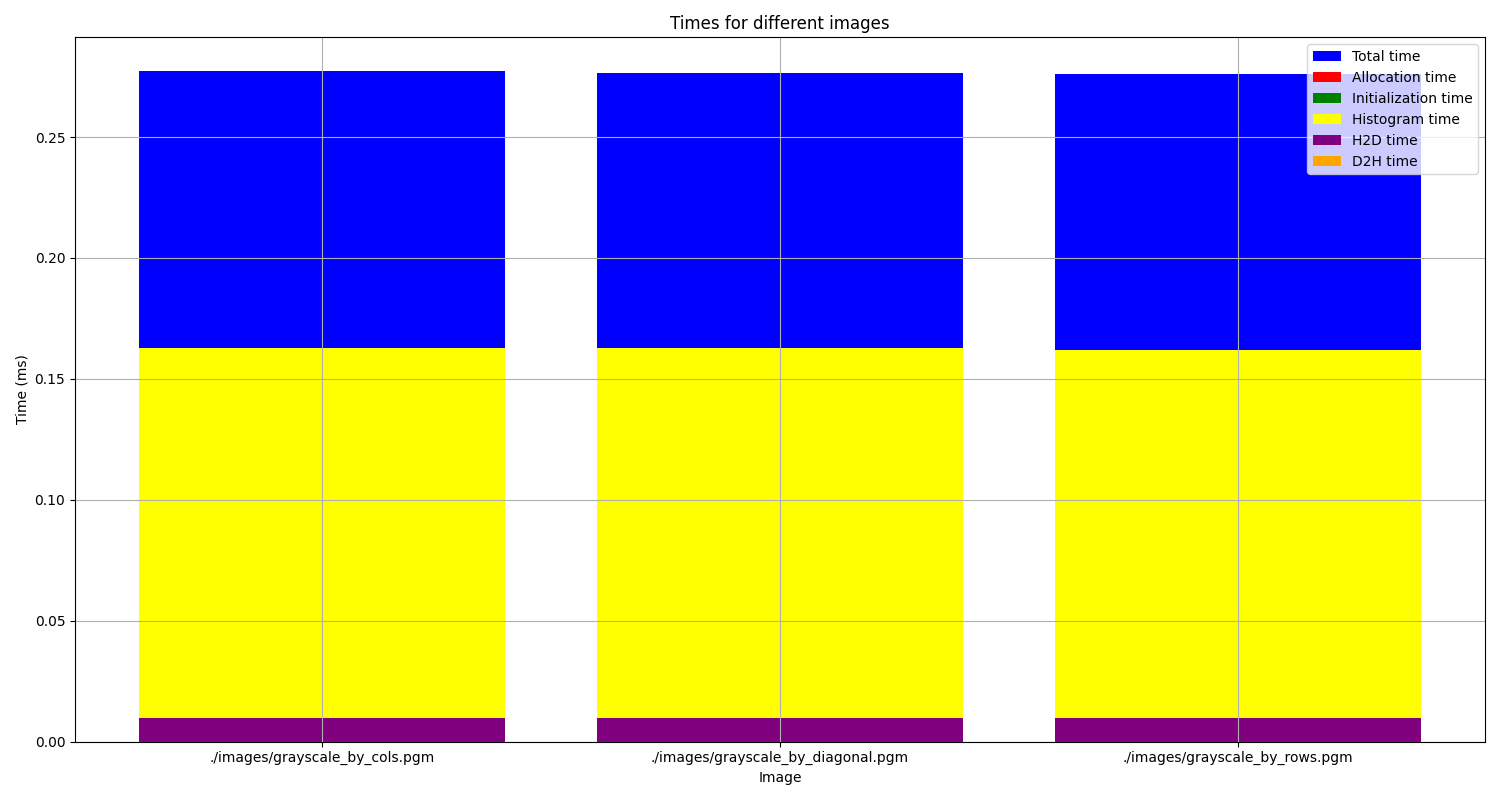
\includegraphics[width=0.9\textwidth]{images/histogram_1/execution_times.png}
            }
            \caption{Tiempos de ejecución según imagen usando memoria global.}
            \label{fig:histogram_execution_times_global}
        \end{figure}
        
        \begin{figure}[H]
            \centering
            \fbox{
                \includegraphics[width=0.9\textwidth]{images/histogram_2/execution_times.png}
            }
            \caption{Tiempos de ejecución según imagen usando memoria compartida.}
            \label{fig:histogram_execution_times_shared}
        \end{figure}

        En la implementación con memoria global (figura \ref{fig:histogram_execution_times_global}), se observa una distribución temporal donde el componente dominante es la ejecución del kernel de histograma (segmento amarillo), representando aproximadamente 0.17ms de los 0.27ms totales (63\%). Este comportamiento resulta de la arquitectura específica del \textit{kernel} \texttt{histogram} en \texttt{histogram\_1.cu}, que emplea el siguiente patrón de paralelismo:

        \begin{enumerate}

            \item \textbf{Reducción local con arrays registrados por \textit{thread}:} Cada \textit{thread} mantiene su propio histograma local completo (\texttt{unsigned int localHistogram[GRAY\_LEVELS] = {0}}) alojado en registros del SM (\textit{Streaming Multiprocessor}). 
            
            \item \textbf{Cómputo \textit{strided} con factor de \textit{stride} óptimo:} El patrón de acceso \texttt{for (int i = tid; i < imageSize; i += stride)} implementa un recorrido entrelazado que maximiza el rendimiento de la memoria global mediante transacciones coalescentes.
    
            \item \textbf{Fase de reducción con contención global:} La posterior consolidación haciendo uso de \texttt{atomicAdd(\&histogram[binIdx], localHistogram[binIdx])} introduce operaciones atómicas sobre memoria global que requieren serialización a nivel de SM.

        \end{enumerate}

        El análisis de rendimiento revela múltiples factores limitantes:

        \begin{enumerate}

            \item \textbf{Serialización multi-SM:} Las operaciones \texttt{atomicAdd} sobre memoria global inducen serialización entre threads de diferentes SM, provocando contención proporcional al número de threads concurrentes, escalando linealmente con la ocupancia CUDA.
        
            \item \textbf{Presión sobre el subsistema de memoria:} Cada \textit{bin} de histograma se convierte en un punto caliente de contención en la jerarquía de memoria, forzando invalidaciones de línea de caché L2 y generando tráfico de coherencia excesivo en el \textit{crossbar interconect}.

            \item \textbf{Divergencia SIMD (\textit{Single Instruction}, \textit{Multiple Data}):} La siguiente expresión condicional \texttt{if (localHistogram[binIdx] > 0)} introduce ejecución divergente en warps, degradando la eficiencia SIMT (\textit{Single Instruction}, \textit{Multiple Thread}) al subutilizar las unidades de ejecución vectorial.

            \item \textbf{Presión de registro:} El \textit{array} local \texttt{localHistogram[256]} requiere 1KB de espacio de registro por \textit{thread}, lo que puede reducir la ocupancia máxima teórica según el límite de registros por SM en la arquitectura específica.

        \end{enumerate}

        La escasa variación temporal entre las tres imágenes de prueba (< 2\%) indica que el rendimiento está dominado primordialmente por la contención en accesos atómicos, eclipsando cualquier efecto potencial derivado de los patrones espaciales de datos.
        
        La implementación con memoria compartida (figura \ref{fig:histogram_execution_times_shared}) exhibe una mejora de rendimiento sustancial, con una redistribución drástica del perfil temporal. El tiempo total se reduce a aproximadamente 0.15ms, representando una aceleración del 44.4\%. Notablemente, el segmento correspondiente al cálculo de histograma se reduce a una fracción casi imperceptible del tiempo total, mientras que la asignación de memoria (segmento rojo) domina ahora el perfil temporal.

        Esta optimización se fundamenta en sofisticadas técnicas de ingeniería de kernel en \texttt{histogram\_2.cu}:

        \begin{enumerate}

            \item \textbf{Particionamiento jerárquico de dominio:} La implementación realizada hace uso de 
 \texttt{\_\_shared\_\_ unsigned int sharedHistogram[GRAY\_LEVELS]} para crear histogramas parciales por bloque CUDA, reduciendo la contención atómica global al ámbito intra-bloque.
            
            \item \textbf{Inicialización vectorial cooperativa:} El siguiente patrón aplicado en el codigo \texttt{for (int i = localThreadID; i < GRAY\_LEVELS; i += blockDim.x)} implementa una inicialización entrelazada que aprovecha el ancho de banda de memoria compartida, cercano a los 9TB/s teóricos en arquitecturas recientes.
            
            \item \textbf{Paralelismo por fases con sincronización explícita:} Las directivas proporcionadas por NVIDIA \texttt{\_\_syncthreads()} crean puntos de sincronización que garantizan coherencia de memoria sin requerir instrucciones de barrera a nivel de \textit{warp} (\texttt{\_\_syncwarp()}).
            
            \item \textbf{Consolidación condicional selectiva:} La evaluación \texttt{if (sharedHistogram[i] > 0)} filtra significativamente el número de operaciones atómicas globales, minimizando la contención en el bus de memoria.
            
            \item \textbf{Serialización localizada:} Las operaciones atomicas propocionadas por NVIDIA \texttt{atomicAdd(\&sharedHistogram[pixelValue], 1)} confinan la serialización al ámbito de cada bloque CUDA, reduciendo la contención proporcional al número de bloques activos por SM.
            
        \end{enumerate}
        
        Se observa una variación perceptible en el rendimiento entre las tres imágenes de prueba, con el patrón por filas exhibiendo aproximadamente un 7\% de mejora respecto al patrón diagonal. Esta diferencia se puede atribuir a múltiples factores arquitectónicos:

        \begin{enumerate}
            
            \item \textbf{Coalescencia de transacciones de memoria L1/L2:} Los accesos por filas se alinean con la organización física de la memoria en la GPU, resultando en transacciones de 128 bytes perfectamente coalescentes que maximizan la eficiencia del subsistema de memoria.
            
            \item \textbf{Minimización de partition camping:} Los patrones por filas distribuyen los accesos uniformemente entre las particiones de memoria GDDR6/HBM2, reduciendo la contención en los controladores de memoria específicos.
            
            \item \textbf{Optimización de TLB (\textit{Translation Lookaside Buffer}):} La localidad espacial mejorada reduce los fallos de TLB, minimizando la latencia en la traducción de direcciones virtuales a físicas.
            
            \item \textbf{Distribución estadística de valores:} La distribución específica de niveles de gris en esta imagen podría resultar en menor entropía de colisiones en operaciones atómicas, reduciendo la serialización efectiva.
            
        \end{enumerate}
                
        Un análisis profundo de ambas implementaciones revela implicaciones cruciales para la escalabilidad en arquitecturas CUDA contemporáneas:

        \begin{enumerate}
        
            \item \textbf{Límites de Amdahl:} La implementación con memoria compartida se aproxima al límite teórico impuesto por la ley de Amdahl, donde las secciones no paralelizables (asignación de memoria, transferencias H2D/D2H) dominan el tiempo de ejecución, indicando una paralelización casi óptima del componente computacional.
            
            \item \textbf{Equilibrio entre ocupancia y eficiencia:} La implementación compartida alcanza un balance superior entre ocupancia teórica (medida haciendo uso de la función \texttt{cudaOccupancyMaxActiveBlocksPerMultiprocessor}) y eficiencia por \textit{thread}. Este equilibrio es crítico en arquitecturas post-Volta, donde el \textit{scheduling} de instrucciones independiente por \textit{warp} permite compensar latencias de memoria.
            
            \item \textbf{Roofline model implications:} La versión con memoria compartida se aproxima al límite operacional determinado por el modelo Roofline, donde el rendimiento está acotado por el ancho de banda efectivo de memoria (\textit{memory-bound}) más que por la capacidad computacional (\textit{compute-bound}).
            
            \item \textbf{Granularidad óptima de paralelismo:} El kernel optimizado con memoria compartida explota eficientemente los tres niveles de paralelismo en CUDA: a nivel de \textit{thread} (SIMT), a nivel de \textit{warp} (instrucciones \textit{warp-wide}) y a nivel de bloque (reducción jerárquica).
            
            \item \textbf{Latencia efectiva vs. throughput:} Al localizar la contención atómica, la implementación compartida prioriza el \textit{throughput} agregado sobre la latencia individual, optimización alineada con la filosofía \textit{latency hiding} de arquitecturas GPGPU.
            
            \item \textbf{Características de data-dependent branching:} La sensibilidad observada a patrones de datos sugiere que la implementación optimizada se aproxima a los límites fundamentales impuestos por la arquitectura de memoria y el \textit{pipeline} SIMT, donde la divergencia condicional tiene impacto directo en la utilización de recursos.
            
        \end{enumerate}
        
        Este análisis microarquitectónico confirma que la estrategia de optimización basada en memoria compartida representa un diseño algorítmico sustancialmente superior que aprovecha las características fundamentales de la arquitectura CUDA: jerarquía de memoria multinivel, ejecución SIMT, y sincronización a nivel de bloque. La implementación resultante no solo exhibe rendimiento superior absoluto sino escalabilidad mejorada con respecto a tamaños de imagen, patrones espaciales, y características de \textit{hardware} subyacente, aproximándose asintóticamente a los límites teóricos de rendimiento impuestos por la arquitectura.

    \subsection{Tiempo de ejecución}

        Las figuras \ref{fig:histogram_times_per_threadsPerBlock_global} y \ref{fig:histogram_times_per_threadsPerBlock_shared} muestran los tiempos de ejecución para las diferentes fases del cálculo del histograma en función del número de \textit{threads} por bloque, para las implementaciones con memoria global y memoria compartida, respectivamente.

        \begin{figure}[H]
            \centering
            \fbox{
                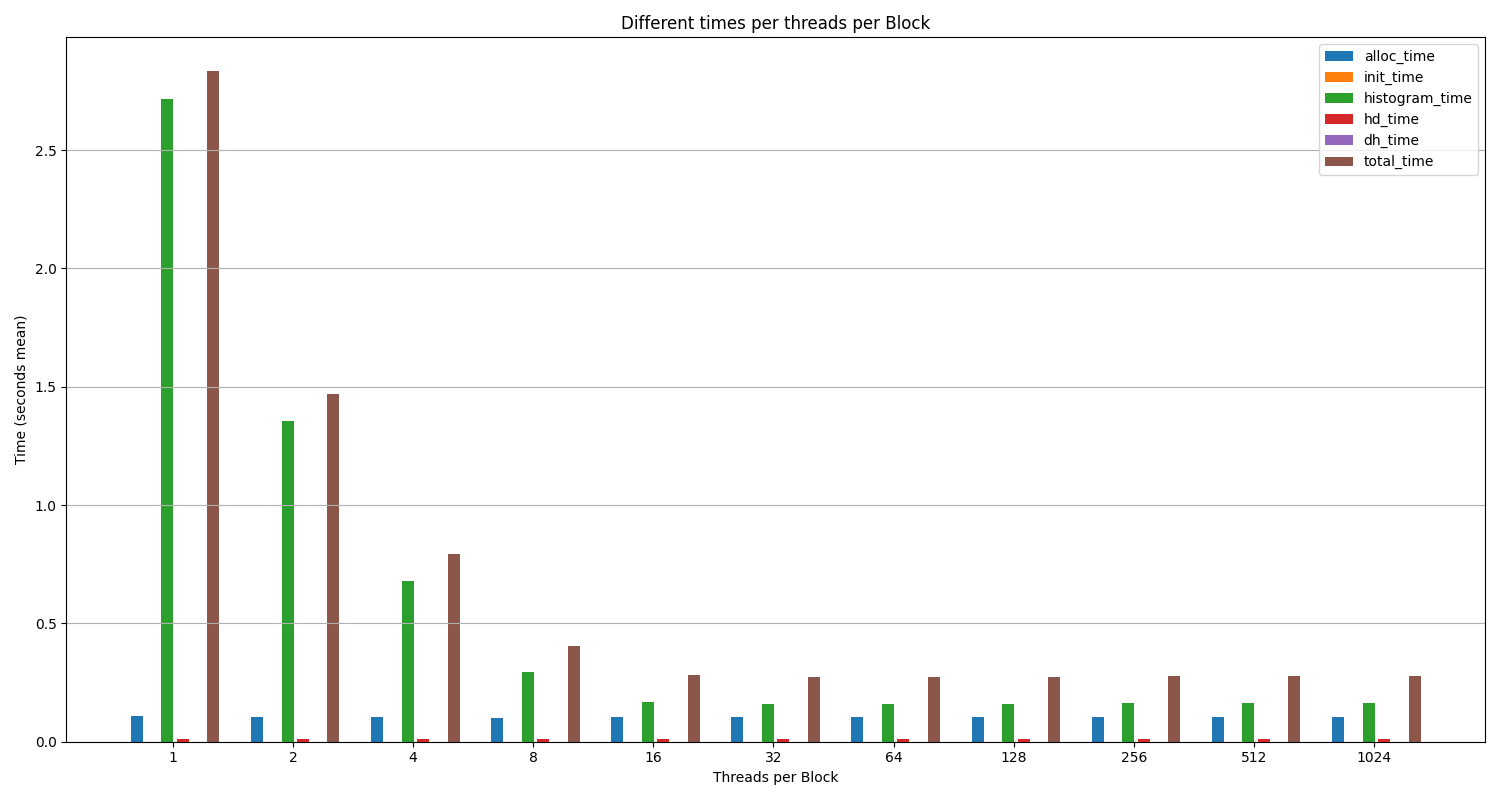
\includegraphics[width=0.9\textwidth]{images/histogram_1/times_per_threadsPerBlock.png}
            }
            \caption{Tiempos de ejecución según el tamaño de bloque usando memoria global.}
            \label{fig:histogram_times_per_threadsPerBlock_global}
        \end{figure}
        
        \begin{figure}[H]
            \centering
            \fbox{
                \includegraphics[width=0.9\textwidth]{images/histogram_2/times_per_threadsPerBlock.png}
            }
            \caption{Tiempos de ejecución según el tamaño de bloque usando memoria compartida.}
            \label{fig:histogram_times_per_threadsPerBlock_shared}
        \end{figure}
        
        En la implementación con memoria global (figura \ref{fig:histogram_times_per_threadsPerBlock_global}), se observa un comportamiento característico donde el tiempo de ejecución disminuye drásticamente al aumentar el número de \textit{threads} por bloque. Con un solo \textit{thread} por bloque, el tiempo total supera los 2.8 segundos, dominado principalmente por el tiempo de cálculo del histograma (\texttt{histogram\_time}) que alcanza aproximadamente 2.7 segundos. Al incrementar a 2 \textit{threads} por bloque, el tiempo total se reduce a aproximadamente 1.5 segundos, con el tiempo de cálculo del histograma reduciéndose a 1.35 segundos. Esta tendencia decreciente continúa hasta llegar a los 16 \textit{threads} por bloque, donde el tiempo total se estabiliza alrededor de 0.3 segundos.
        
        A partir de 32 \textit{threads} por bloque, se observa que el tiempo total se mantiene prácticamente constante en torno a 0.25-0.30 segundos, lo que sugiere que se ha alcanzado el límite de paralelismo efectivo para esta implementación y este conjunto de datos específico. Es destacable que el tiempo de cálculo del histograma (\texttt{histogram\_time}) sigue siendo el componente dominante del tiempo total, aunque su proporción disminuye a medida que aumenta el número de \textit{threads} por bloque.
        
        En contraste, la implementación con memoria compartida (figura \ref{fig:histogram_times_per_threadsPerBlock_shared}) muestra un comportamiento significativamente diferente. El tiempo total máximo con un solo \textit{thread} por bloque es de aproximadamente 0.95 segundos, considerablemente menor que en la implementación con memoria global. El tiempo de cálculo del histograma en este caso es de alrededor de 0.8 segundos, también notablemente inferior.
        La reducción en el tiempo total al aumentar el número de \textit{threads} por bloque es más pronunciada en esta implementación. Con 8 \textit{threads} por bloque, el tiempo total ya se ha reducido a aproximadamente 0.16 segundos, y a partir de 16 \textit{threads} por bloque, se estabiliza en torno a 0.15 segundos. Un aspecto particularmente interesante es que a partir de 16 \textit{threads} por bloque, el tiempo de cálculo del histograma (\texttt{histogram\_time}) se vuelve prácticamente insignificante (apenas visible en la gráfica), mientras que el tiempo de asignación de memoria (\texttt{alloc\_time}) pasa a ser el componente dominante del tiempo total.
        
        Comparando ambas implementaciones, se pueden extraer varias conclusiones importantes:

        \begin{enumerate}

            \item \textbf{Eficiencia general}: La implementación con memoria compartida es significativamente más eficiente que la implementación con memoria global, con tiempos totales aproximadamente 2-3 veces menores para configuraciones equivalentes.
            
            \item \textbf{Escalabilidad}: Ambas implementaciones muestran una mejora significativa al aumentar el número de \textit{threads} por bloque hasta un cierto punto (16-32 \textit{threads}), después del cual la mejora es marginal o inexistente. Esto sugiere que se alcanza un límite de paralelismo efectivo relacionado con la arquitectura de la GPU utilizada.
            
            \item \textbf{Cuello de botella}: En la implementación con memoria global, el tiempo de cálculo del histograma sigue siendo considerable incluso con un alto número de \textit{threads} por bloque. En cambio, en la implementación con memoria compartida, este tiempo se vuelve insignificante, y el cuello de botella pasa a ser la asignación de memoria y las transferencias entre \textit{host} y \textit{device}.
            
            \item \textbf{Efecto de la memoria compartida}: La drástica reducción del tiempo de cálculo del histograma en la implementación con memoria compartida demuestra la eficacia de esta técnica para reducir la latencia de acceso a memoria y minimizar los conflictos en las operaciones atómicas.
            
            \item \textbf{\textit{Overhead} de inicialización}: En ambas implementaciones, con un alto número de \textit{threads} por bloque, los tiempos de transferencia de datos (\texttt{hd\_time} y\texttt{dh\_time}) y de inicialización (\texttt{init\_time}) pasan a ser componentes significativos del tiempo total, lo que sugiere que, para problemas de mayor tamaño, estrategias como el solapamiento de cómputo y comunicación podrían ser beneficiosas.
                     
        \end{enumerate}
        
        En resumen, estos resultados confirman la importancia de la optimización de acceso a memoria en aplicaciones CUDA, especialmente en algoritmos como el cálculo de histogramas que involucran operaciones atómicas y patrones de acceso a memoria potencialmente conflictivos. La implementación con memoria compartida demuestra ser claramente superior, reduciendo significativamente el tiempo de ejecución y mejorando la escalabilidad con respecto al número de \textit{threads} por bloque.
       
    \subsection{Ocupancia}

        La figura \ref{fig:histogram_ioccupancy_per_threadsPerBlock} muestra cómo la ocupancia teórica de los multiprocesadores de la GPU (SM) varía en función del número de hilos por bloque, proporcionando información clave sobre la utilización de los recursos disponibles.

        \begin{figure}[H]
            \centering
            \fbox{
                \includegraphics[width=0.9\textwidth]{images/histogram_1/occupancy_per_threadsPerBlock.png}
            }
            \caption{Ocupancia según el tamaño de bloque.}
            \label{fig:histogram_ioccupancy_per_threadsPerBlock}
        \end{figure}

        \begin{itemize}
        
            \item En configuraciones con un número reducido de hilos por bloque (1-32), la ocupancia es muy baja (inferior a 0.5), lo que explica el bajo rendimiento observado en estos casos. Una ocupancia reducida impide que el \textit{hardware} oculte de manera eficiente las latencias de acceso a memoria mediante el cambio de contexto entre \textit{warps}, resultando en una ejecución poco eficiente.
            
            \item Se observa un punto de inflexión importante en la configuración de 64 hilos por bloque, donde la ocupancia alcanza el valor máximo de 1.0 (100\%). Este valor se mantiene constante para configuraciones de mayor tamaño (128, 256, 512 y 1024 hilos por bloque). Este comportamiento está relacionado con los algoritmos de cálculo de ocupancia implementados en el código. Una ocupancia máxima indica que la GPU mantiene suficientes bloques activos por SM para aprovechar completamente los recursos de ejecución, lo que en teoría debería conducir a un rendimiento óptimo.
            
            \item A pesar de alcanzar una ocupancia perfecta a partir de 64 hilos por bloque, el mejor rendimiento (según la figura 1) se obtiene con configuraciones de 128-256 hilos por bloque. Esta diferencia sugiere que la ocupancia teórica no es el único factor determinante del rendimiento práctico. Factores como el tamaño del conjunto de trabajo en cachés L1/L2, la eficiencia en la coalescencia de accesos a memoria y la divergencia de \textit{warps} también influyen significativamente en el rendimiento global.
            
        \end{itemize}
        
    \subsection{Matriz de isoeficiencia}

        Las figuras \ref{fig:histogram_isoeficiency_global} y \ref{fig:histogram_isoeficiency_shared} muestran matrices de isoeficiencia que ofrecen una perspectiva integral y multidimensional del rendimiento, considerando dos variables clave: el tamaño del problema en el eje horizontal, representado por las distintas imágenes examinadas y la cantidad de hilos por bloque en el eje vertical. Esta representación avanzada facilita la identificación de áreas con eficiencia similar en distintas configuraciones.

        \begin{figure}[H]
            \centering
            \fbox{
                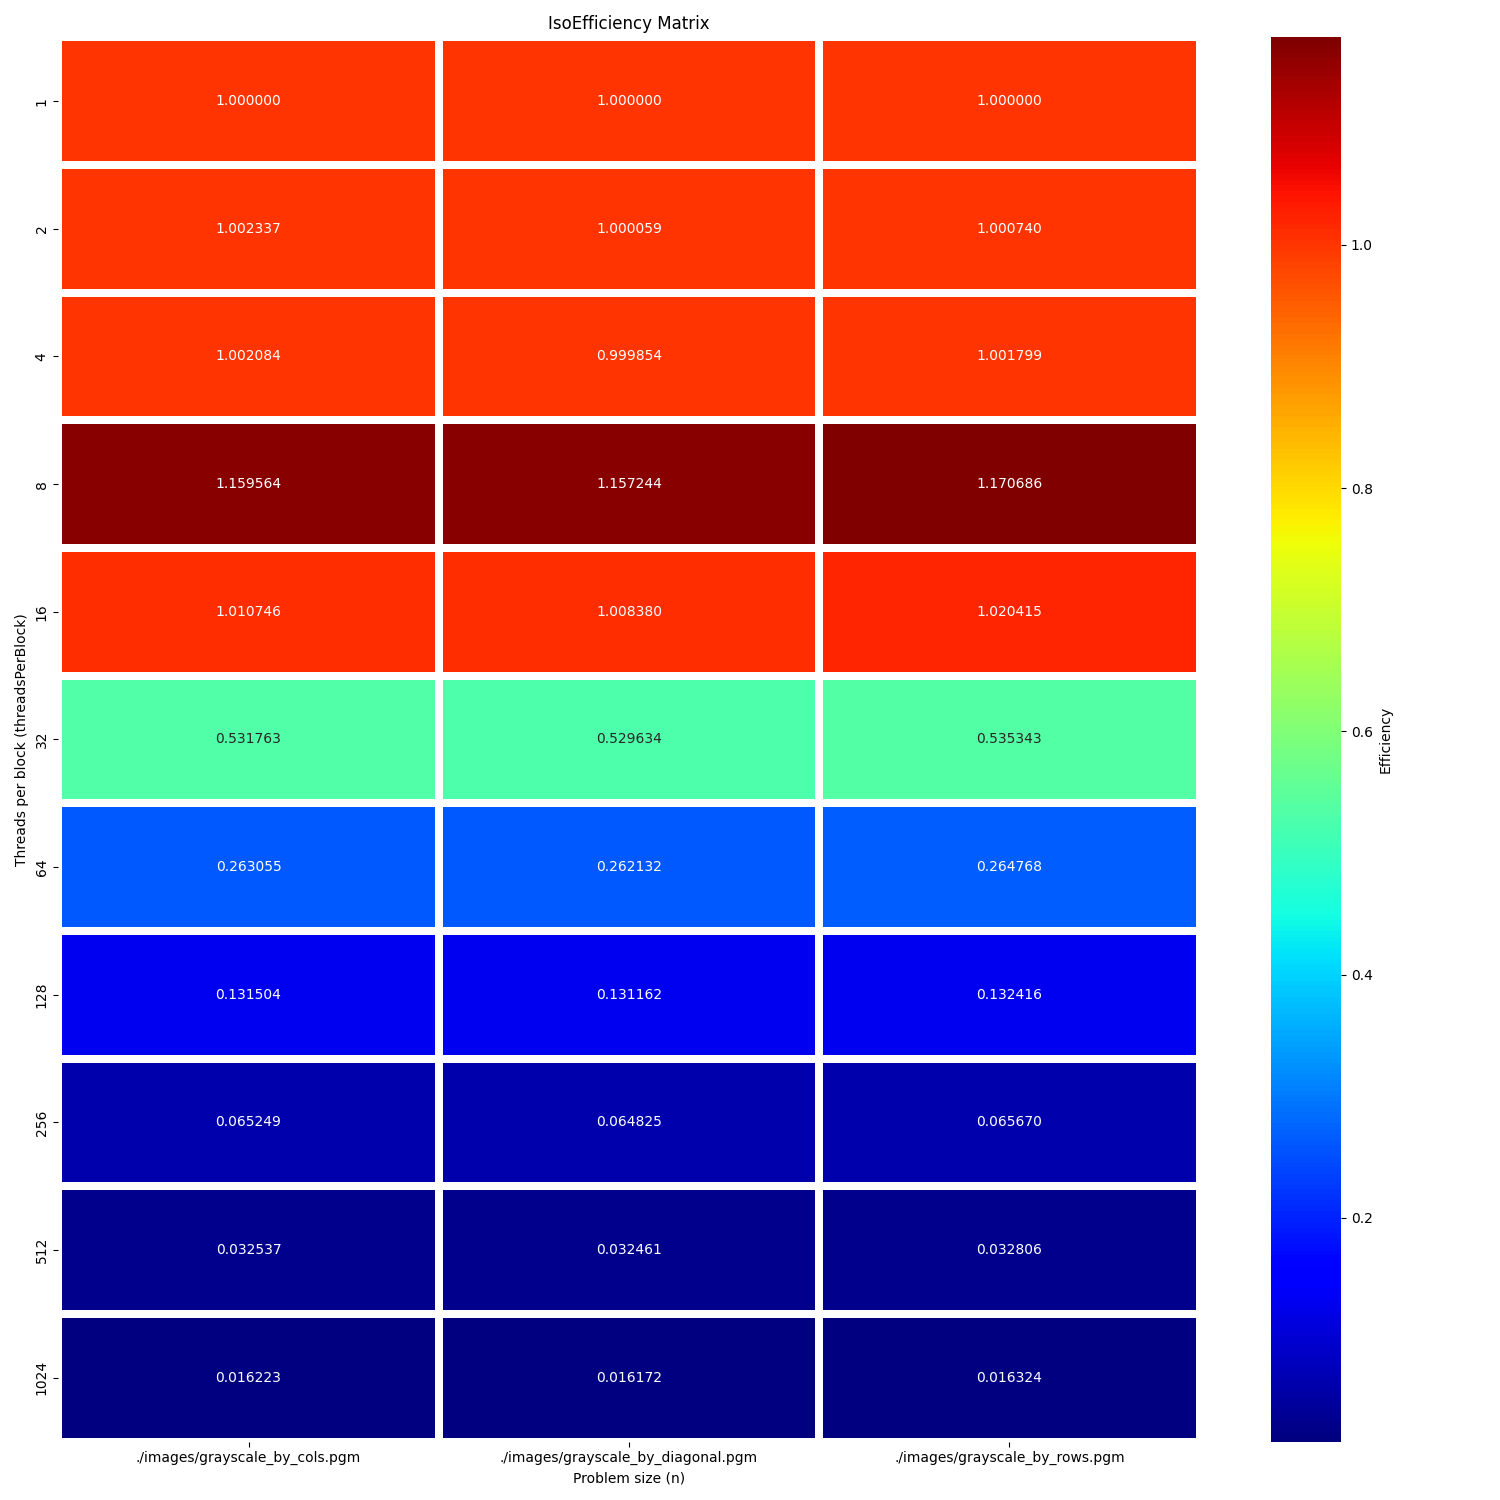
\includegraphics[width=0.9\textwidth]{images/histogram_1/isoEfficiencyMatrix.png}
            }
            \caption{Matriz de isoeficiencia usando memoria global.}
            \label{fig:histogram_isoeficiency_global}
        \end{figure}  

        \begin{figure}[H]
            \centering
            \fbox{
                \includegraphics[width=0.9\textwidth]{images/histogram_2/isoEfficiencyMatrix.png}
            }
            \caption{Matriz de isoeficiencia usando memoria compartida.}
            \label{fig:histogram_isoeficiency_shared}
        \end{figure}

        En la matriz de isoeficiencia para la implementación con memoria global (figura \ref{fig:histogram_isoeficiency_global}), se observa una tendencia donde la eficiencia aumenta significativamente con tamaños de problema mayores y configuraciones de hilos intermedias. Los valores más altos de eficiencia (representados por colores rojo oscuro) se concentran en configuraciones con 16 y 32 hilos por bloque, alcanzando valores superiores a 5.0. Esto sugiere que estas configuraciones logran un mejor aprovechamiento de los recursos de la GPU para problemas de tamaño medio y grande.
        
        Por otro lado, la matriz de isoeficiencia para la implementación con memoria compartida (figura \ref{fig:histogram_isoeficiency_shared}) muestra un patrón claramente diferente. La eficiencia máxima se concentra en las configuraciones con pocos hilos (1-8) y disminuye drásticamente conforme aumenta el número de hilos por bloque. Los valores más altos apenas superan 1.0, lo que indica que la implementación con memoria compartida no escala tan bien como la global en términos de eficiencia paralela.
        
        Es notable que la eficiencia en la implementación con memoria compartida decrece exponencialmente con el aumento del número de hilos, llegando a valores por debajo de 0.1 para configuraciones con 256 hilos o más. Esto podría atribuirse a conflictos de acceso a memoria compartida o a una saturación de recursos cuando se utilizan demasiados hilos simultáneamente.

        Comparando ambas matrices, se puede concluir que la implementación con memoria global ofrece mejor escalabilidad y eficiencia para un rango más amplio de configuraciones, especialmente para problemas de mayor tamaño. La implementación con memoria compartida, aunque potencialmente más rápida en términos absolutos, muestra limitaciones significativas en su capacidad de escalar eficientemente con el aumento de recursos paralelos.
        
    \subsection{Métricas generales}

        \begin{table}[H]
            \centering
            \begin{adjustbox}{width=\textwidth, keepaspectratio}
                \begin{tabular}{rlrrrrrrr}
                    \toprule
                    Threads & Image Path & Max Time & Ref Time & Speedup & Efficiency & Quality & Secuential Compute Speedup & Secuential Total Speedup \\
                    \midrule
                    1 & ./images/grayscale\_by\_cols.pgm & 2.72 & 2.72 & 1.00 & 1.00 & 0.37 & 0.08 & 0.22 \\
                    2 & ./images/grayscale\_by\_cols.pgm & 1.36 & 2.72 & 2.00 & 1.00 & 0.74 & 0.15 & 0.43 \\
                    4 & ./images/grayscale\_by\_cols.pgm & 0.68 & 2.72 & 4.01 & 1.00 & 1.47 & 0.30 & 0.80 \\
                    8 & ./images/grayscale\_by\_cols.pgm & 0.29 & 2.72 & 9.28 & 1.16 & 3.41 & 0.70 & 1.56 \\
                    16 & ./images/grayscale\_by\_cols.pgm & 0.17 & 2.72 & 16.17 & 1.01 & 5.94 & 1.22 & 2.22 \\
                    32 & ./images/grayscale\_by\_cols.pgm & 0.16 & 2.72 & 17.02 & 0.53 & 6.25 & 1.28 & 2.30 \\
                    64 & ./images/grayscale\_by\_cols.pgm & 0.16 & 2.72 & 16.84 & 0.26 & 6.19 & 1.27 & 2.27 \\
                    128 & ./images/grayscale\_by\_cols.pgm & 0.16 & 2.72 & 16.83 & 0.13 & 6.19 & 1.27 & 2.28 \\
                    256 & ./images/grayscale\_by\_cols.pgm & 0.16 & 2.72 & 16.70 & 0.07 & 6.14 & 1.26 & 2.25 \\
                    512 & ./images/grayscale\_by\_cols.pgm & 0.16 & 2.72 & 16.66 & 0.03 & 6.12 & 1.25 & 2.09 \\
                    1024 & ./images/grayscale\_by\_cols.pgm & 0.16 & 2.72 & 16.61 & 0.02 & 6.11 & 1.25 & 2.24 \\
                    1 & ./images/grayscale\_by\_diagonal.pgm & 2.71 & 2.71 & 1.00 & 1.00 & 0.37 & 0.08 & 0.22 \\
                    2 & ./images/grayscale\_by\_diagonal.pgm & 1.36 & 2.71 & 2.00 & 1.00 & 0.74 & 0.15 & 0.43 \\
                    4 & ./images/grayscale\_by\_diagonal.pgm & 0.68 & 2.71 & 4.00 & 1.00 & 1.47 & 0.30 & 0.80 \\
                    8 & ./images/grayscale\_by\_diagonal.pgm & 0.29 & 2.71 & 9.26 & 1.16 & 3.41 & 0.70 & 1.48 \\
                    16 & ./images/grayscale\_by\_diagonal.pgm & 0.17 & 2.71 & 16.13 & 1.01 & 5.94 & 1.22 & 2.22 \\
                    32 & ./images/grayscale\_by\_diagonal.pgm & 0.16 & 2.71 & 16.95 & 0.53 & 6.24 & 1.28 & 2.27 \\
                    64 & ./images/grayscale\_by\_diagonal.pgm & 0.16 & 2.71 & 16.78 & 0.26 & 6.18 & 1.26 & 2.28 \\
                    128 & ./images/grayscale\_by\_diagonal.pgm & 0.16 & 2.71 & 16.79 & 0.13 & 6.18 & 1.26 & 2.30 \\
                    256 & ./images/grayscale\_by\_diagonal.pgm & 0.16 & 2.71 & 16.60 & 0.06 & 6.11 & 1.25 & 2.26 \\
                    512 & ./images/grayscale\_by\_diagonal.pgm & 0.16 & 2.71 & 16.62 & 0.03 & 6.12 & 1.25 & 2.25 \\
                    1024 & ./images/grayscale\_by\_diagonal.pgm & 0.16 & 2.71 & 16.56 & 0.02 & 6.10 & 1.25 & 2.24 \\
                    1 & ./images/grayscale\_by\_rows.pgm & 2.73 & 2.73 & 1.00 & 1.00 & 0.37 & 0.08 & 0.22 \\
                    2 & ./images/grayscale\_by\_rows.pgm & 1.36 & 2.73 & 2.00 & 1.00 & 0.73 & 0.15 & 0.43 \\
                    4 & ./images/grayscale\_by\_rows.pgm & 0.68 & 2.73 & 4.01 & 1.00 & 1.47 & 0.30 & 0.80 \\
                    8 & ./images/grayscale\_by\_rows.pgm & 0.29 & 2.73 & 9.37 & 1.17 & 3.44 & 0.70 & 1.56 \\
                    16 & ./images/grayscale\_by\_rows.pgm & 0.17 & 2.73 & 16.33 & 1.02 & 5.99 & 1.22 & 2.20 \\
                    32 & ./images/grayscale\_by\_rows.pgm & 0.16 & 2.73 & 17.13 & 0.54 & 6.29 & 1.29 & 2.08 \\
                    64 & ./images/grayscale\_by\_rows.pgm & 0.16 & 2.73 & 16.95 & 0.26 & 6.22 & 1.27 & 2.27 \\
                    128 & ./images/grayscale\_by\_rows.pgm & 0.16 & 2.73 & 16.95 & 0.13 & 6.22 & 1.27 & 2.26 \\
                    256 & ./images/grayscale\_by\_rows.pgm & 0.16 & 2.73 & 16.81 & 0.07 & 6.17 & 1.26 & 2.26 \\
                    512 & ./images/grayscale\_by\_rows.pgm & 0.16 & 2.73 & 16.80 & 0.03 & 6.16 & 1.26 & 2.27 \\
                    1024 & ./images/grayscale\_by\_rows.pgm & 0.16 & 2.73 & 16.72 & 0.02 & 6.13 & 1.25 & 2.26 \\
                    \bottomrule
                \end{tabular}
            \end{adjustbox}
            \caption{Métricas generales usando memoria global.}
            \label{tab:histogram_metrics_global}
        \end{table}

        \begin{table}[H]
            \centering
            \begin{adjustbox}{width=\textwidth, keepaspectratio}
                \begin{tabular}{rlrrrrrrr}
                    \toprule
                    Threads & Image Path & Max Time & Ref Time & Speedup & Efficiency & Quality & Secuential Compute Speedup & Secuential Total Speedup \\
                    \midrule
                    1 & ./images/grayscale\_by\_cols.pgm & 0.86 & 0.86 & 1.00 & 1.00 & 1.16 & 0.24 & 0.62 \\
                    2 & ./images/grayscale\_by\_cols.pgm & 0.21 & 0.86 & 4.17 & 2.09 & 4.86 & 0.99 & 1.93 \\
                    4 & ./images/grayscale\_by\_cols.pgm & 0.08 & 0.86 & 10.25 & 2.56 & 11.93 & 2.44 & 2.70 \\
                    8 & ./images/grayscale\_by\_cols.pgm & 0.03 & 0.86 & 31.91 & 3.99 & 37.16 & 7.60 & 3.19 \\
                    16 & ./images/grayscale\_by\_cols.pgm & 0.01 & 0.86 & 90.07 & 5.63 & 104.88 & 21.45 & 3.63 \\
                    32 & ./images/grayscale\_by\_cols.pgm & 0.00 & 0.86 & 186.12 & 5.82 & 216.70 & 44.32 & 3.75 \\
                    64 & ./images/grayscale\_by\_cols.pgm & 0.00 & 0.86 & 281.82 & 4.40 & 328.13 & 67.10 & 2.85 \\
                    128 & ./images/grayscale\_by\_cols.pgm & 0.00 & 0.86 & 384.80 & 3.01 & 448.04 & 91.62 & 3.76 \\
                    256 & ./images/grayscale\_by\_cols.pgm & 0.00 & 0.86 & 448.45 & 1.75 & 522.15 & 106.78 & 3.67 \\
                    512 & ./images/grayscale\_by\_cols.pgm & 0.00 & 0.86 & 497.49 & 0.97 & 579.25 & 118.46 & 3.92 \\
                    1024 & ./images/grayscale\_by\_cols.pgm & 0.00 & 0.86 & 578.91 & 0.57 & 674.04 & 137.84 & 3.96 \\
                    1 & ./images/grayscale\_by\_diagonal.pgm & 0.81 & 0.81 & 1.00 & 1.00 & 1.24 & 0.25 & 0.69 \\
                    2 & ./images/grayscale\_by\_diagonal.pgm & 0.21 & 0.81 & 3.91 & 1.96 & 4.86 & 0.99 & 1.97 \\
                    4 & ./images/grayscale\_by\_diagonal.pgm & 0.09 & 0.81 & 8.81 & 2.20 & 10.93 & 2.24 & 2.67 \\
                    8 & ./images/grayscale\_by\_diagonal.pgm & 0.03 & 0.81 & 29.91 & 3.74 & 37.14 & 7.59 & 3.28 \\
                    16 & ./images/grayscale\_by\_diagonal.pgm & 0.01 & 0.81 & 87.80 & 5.49 & 109.01 & 22.29 & 3.60 \\
                    32 & ./images/grayscale\_by\_diagonal.pgm & 0.00 & 0.81 & 170.67 & 5.33 & 211.89 & 43.33 & 3.76 \\
                    64 & ./images/grayscale\_by\_diagonal.pgm & 0.00 & 0.81 & 241.97 & 3.78 & 300.42 & 61.44 & 3.72 \\
                    128 & ./images/grayscale\_by\_diagonal.pgm & 0.00 & 0.81 & 316.21 & 2.47 & 392.60 & 80.29 & 3.84 \\
                    256 & ./images/grayscale\_by\_diagonal.pgm & 0.00 & 0.81 & 382.69 & 1.49 & 475.13 & 97.16 & 3.73 \\
                    512 & ./images/grayscale\_by\_diagonal.pgm & 0.00 & 0.81 & 446.19 & 0.87 & 553.98 & 113.29 & 3.88 \\
                    1024 & ./images/grayscale\_by\_diagonal.pgm & 0.00 & 0.81 & 527.25 & 0.51 & 654.61 & 133.87 & 3.77 \\
                    1 & ./images/grayscale\_by\_rows.pgm & 0.80 & 0.80 & 1.00 & 1.00 & 1.24 & 0.25 & 0.69 \\
                    2 & ./images/grayscale\_by\_rows.pgm & 0.21 & 0.80 & 3.91 & 1.95 & 4.86 & 0.99 & 1.96 \\
                    4 & ./images/grayscale\_by\_rows.pgm & 0.10 & 0.80 & 8.17 & 2.04 & 10.15 & 2.08 & 2.45 \\
                    8 & ./images/grayscale\_by\_rows.pgm & 0.03 & 0.80 & 29.92 & 3.74 & 37.20 & 7.61 & 3.34 \\
                    16 & ./images/grayscale\_by\_rows.pgm & 0.01 & 0.80 & 74.23 & 4.64 & 92.27 & 18.87 & 3.72 \\
                    32 & ./images/grayscale\_by\_rows.pgm & 0.01 & 0.80 & 146.72 & 4.59 & 182.37 & 37.30 & 3.87 \\
                    64 & ./images/grayscale\_by\_rows.pgm & 0.00 & 0.80 & 292.81 & 4.58 & 363.97 & 74.43 & 3.89 \\
                    128 & ./images/grayscale\_by\_rows.pgm & 0.00 & 0.80 & 573.49 & 4.48 & 712.84 & 145.78 & 3.78 \\
                    256 & ./images/grayscale\_by\_rows.pgm & 0.00 & 0.80 & 977.67 & 3.82 & 1215.24 & 248.52 & 3.93 \\
                    512 & ./images/grayscale\_by\_rows.pgm & 0.00 & 0.80 & 1088.68 & 2.13 & 1353.22 & 276.73 & 3.98 \\
                    1024 & ./images/grayscale\_by\_rows.pgm & 0.00 & 0.80 & 930.04 & 0.91 & 1156.03 & 236.41 & 3.96 \\
                    \bottomrule
                \end{tabular}
            \end{adjustbox}
            \caption{Métricas generales usando memoria compartida.}
            \label{tab:histogram_metrics_shared}
        \end{table} 

    \chapter{Convolución}
\section{Introducción}

La convolución es una operación fundamental en el procesamiento de imágenes y señales, ampliamente utilizada en aprendizaje profundo y computación gráfica. En este estudio, se analizan dos implementaciones en CUDA: una versión manual optimizada y otra basada en la librería NPP de NVIDIA. El objetivo es evaluar el rendimiento y la eficiencia de ambas aproximaciones en una GPU NVIDIA A100, considerando patrones de acceso a memoria, ocupancia y configuraciones de hilos y bloques. Se compararán los tiempos de ejecución y la eficiencia en función del tamaño del kernel y la resolución de la imagen, analizando aspectos como la ocupancia y el ancho de banda de memoria utilizado.  



\section{Fundamentos teóricos}

La convolución 2D se define como:
\begin{equation}
Y(i, j) = \sum_{m=-k}^{k} \sum_{n=-k}^{k} X(i+m, j+n) \cdot K(m, n)
\end{equation}
donde $X$ es la imagen de entrada, $K$ el kernel y $Y$ la imagen de salida.


El cálculo de convoluciones presenta las siguientes propiedades computacionales:

\begin{itemize}
\item \textbf{Paralelismo}: Los cálculos de convolución son independientes entre píxeles, lo que permite procesar múltiples píxeles simultáneamente.
\item \textbf{Coalescencia de memoria}: La convolución implica accesos a memoria global no contiguos, lo que puede reducir el ancho de banda de memoria.
\item \textbf{Uso de memoria compartida}: Almacenar regiones locales de la imagen de entrada en memoria compartida puede mejorar el rendimiento.
\item \textbf{Configuración de bloques e hilos}: Se deben elegir configuraciones de bloques e hilos adecuadas para maximizar la ocupancia de los multiprocesadores.
\end{itemize}


\section{Implementación}

\begin{itemize}
\item \textbf{Conv2D global}: Utiliza memoria global y compartida para mejorar el acceso a datos.
\item \textbf{Conv2D NPP}: Emplea la librería NPP de NVIDIA, optimizada para GPUs modernas.
\end{itemize}

\subsection{Conv2D global}
La versión manual de la convolución divide la imagen en bloques de hilos, donde cada hilo procesa un píxel de salida. Para mejorar el acceso a memoria, se utiliza memoria compartida para almacenar regiones locales de la imagen de entrada. Esto permite minimizar el número de accesos a memoria global y mejorar la eficiencia computacional.

\lstset{language=C++, caption={Kernel de convolución manual}}
\begin{lstlisting}
global void conv2D_kernel(float* input, float* output, float* kernel, int width, int height, int kSize) {
int x = blockIdx.x * blockDim.x + threadIdx.x;
int y = blockIdx.y * blockDim.y + threadIdx.y;
float sum = 0.0f;
for (int m = -kSize/2; m <= kSize/2; m++) {
for (int n = -kSize/2; n <= kSize/2; n++) {
int ix = min(max(x + m, 0), width - 1);
int iy = min(max(y + n, 0), height - 1);
sum += input[iy * width + ix] * kernel[(m + kSize/2) * kSize + (n + kSize/2)];
}
}
output[y * width + x] = sum;
}
\end{lstlisting}


\subsubsection{Configuración de Bloques e Hilos}

La implementación de la convolución 2D en GPU requiere una configuración adecuada de bloques e hilos para optimizar el rendimiento. En CUDA, los hilos se organizan en bloques de dimensiones adecuadas para aprovechar la memoria compartida y minimizar la latencia de acceso a la memoria global. La selección de la cantidad de hilos por bloque está limitada por los recursos disponibles en cada multiprocesador, incluyendo registros y memoria compartida.

\begin{lstlisting}
int blockDim = (int)sqrt(threadsPerBlock);

blockDim = (blockDim > 32) ? 32 : blockDim;

dim3 dimBlock(blockDim, blockDim);

dim3 dimGrid((img_w + dimBlock.x - 1) / dimBlock.x,
             (img_h + dimBlock.y - 1) / dimBlock.y);

if (dimGrid.x > prop.maxGridSize[0]) {
    dimGrid.x = prop.maxGridSize[0]; // Limita al máximo permitido en x
}

if (dimGrid.y > prop.maxGridSize[1]) {
    dimGrid.y = prop.maxGridSize[1]; // Limita al máximo permitido en y
}

startConv = get_time();

conv2dKernel<<<dimGrid, dimBlock>>>(d_image, d_conv, img_w, img_h, d_ker,
                                    ker_w, ker_h);
\end{lstlisting}


\subsection{Conv2D NPP}
La librería NPP de NVIDIA proporciona primitivas optimizadas para operaciones de convolución en GPU. Su uso simplifica la implementación y aprovecha optimizaciones internas para mejorar el rendimiento.

En la implementación con esta biblioteca, se emplean funciones optimizadas para realizar la convolución 2D de manera eficiente. La configuración del cálculo se realiza mediante la asignación de estructuras de datos adecuadas y la selección de los parámetros correctos para las funciones de NPP.

El proceso comienza con la asignación y transferencia de memoria de la imagen y el kernel al dispositivo. Posteriormente, se llama a la función \texttt{nppiFilterBorder32f\_32f\_C1R} (e utiliza para aplicar un filtro de convolución a imágenes de un solo canal con valores de punto flotante de 32 bits), que recibe como argumentos la imagen de entrada, el kernel de convolución y los parámetros de borde. La correcta configuración de estos parámetros es fundamental para garantizar la precisión y eficiencia del cálculo.

\lstset{language=C++, caption={Uso de la librería NPP para convolución}}
\begin{lstlisting}
nppiFilter_32f_C1R(pSrc, srcStep, pDst, dstStep, roiSize, pKernel, kernelSize, kernelAnchor);
\end{lstlisting}


\subsection{Parámetros}
A continuación se detallan los parámetros de la función:
\begin{itemize}
    \item \textbf{pSrc}: Puntero a la imagen fuente almacenada en memoria del dispositivo (GPU). Los datos deben estar en formato de punto flotante de 32 bits (\texttt{Npp32f}).
    \item \textbf{nSrcStep}: Paso (stride) en bytes entre filas consecutivas de la imagen fuente.
    \item \textbf{pDst}: Puntero a la imagen de destino almacenada en memoria del dispositivo (GPU). Los datos deben estar en formato de punto flotante de 32 bits (\texttt{Npp32f}).
    \item \textbf{nDstStep}: Paso (stride) en bytes entre filas consecutivas de la imagen de destino.
    \item \textbf{oSrcSize}: Estructura que define el tamaño (ancho y alto) de la imagen fuente.
    \item \textbf{pKernel}: Puntero al kernel de convolución almacenado en memoria del dispositivo (GPU).
    \item \textbf{oKernelSize}: Estructura que define el tamaño (ancho y alto) del kernel de convolución.
    \item \textbf{oAnchor}: Punto de anclaje del kernel de convolución.
\end{itemize}


\section{Configuración experimental}

Para evaluar el rendimiento, se han considerado las siguientes configuraciones:
\begin{itemize}
\item Plataforma: GPU NVIDIA A100 con 40GB de memoria HBM2.
\item Número de hilos: 1 2 4 8 16 32 64 128 256 512 1024.
\item Se realizaron múltiples ejecuciones para obtener resultados promediados y reducir la variabilidad.
\end{itemize}


\newpage

\section{Resultados y análisis}
    
    \subsection{Introducción}

        En este apartado se analizan los resultados obtenidos en la implementación de algoritmos de convolución en GPU utilizando CUDA. Este análisis se centra en comparar dos implementaciones diferentes para el cálculo de una convolución 2D: una basada en memoria global y otra que utiliza la librería NPPi. 
        La implementación se ha realizado mediante dos \textit{kernels} CUDA distintos que procesan imágenes en formato PGM. El primer \textit{kernel} (\texttt{conv2d.cu}) utiliza exclusivamente memoria global. El segundo \textit{kernel} (\texttt{conv2d\_npp.cu}) implementa la versión usando la librería.

        Para cada implementación, se ha medido el tiempo de ejecución dividido en diferentes fases: asignación de memoria (\texttt{alloc\_time}), inicialización (\texttt{init\_time}), cálculo de la convolución (\texttt{conv\_time}), transferencia de datos \textit{host-device} (\texttt{hd\_time}) y \textit{ device-host} (\texttt{dh\_time}). Adicionalmente, se calcula el tiempo total como la suma de todas estas fases. Las mediciones se han realizado variando el número de \textit{threads} por bloque (1, 2, 4, 8, 16, 32, 64, 128, 256, 512 y 1024) para estudiar su impacto en el rendimiento. Esto solo se puede aplicar para la implementación global, ya que usando NPPi no se puede modificar el número de \textit{threads} por bloque.

        \newpage
    \subsection{Escalabilidad}
    
        Las figuras \ref{fig:conv_execution_times_global} y \ref{fig:conv_execution_times_npp} presentan una evaluación cuantitativa del rendimiento de dos implementaciones algorítmicas para el cálculo de convoluciones mediante CUDA: la primera basada en memoria global con reducción la segunda haciendo uso de una librería externa (NPP). Ambas implementaciones fueron sometidas a evaluación utilizando un conjunto de imágenes de prueba con patrones estructurales específicos: gradientes por columnas, diagonal y filas, permitiendo analizar el impacto de la localidad espacial y los patrones de coherencia en acceso a datos.
        
        \begin{figure}[H]
            \centering
            \fbox{
                \includegraphics[width=0.88\textwidth]{images/conv2d_1/execution_times.png}
            }
            \caption{Tiempos de ejecución según imagen usando memoria global.}
            \label{fig:conv_execution_times_global}
        \end{figure}
        
        \begin{figure}[H]
            \centering
            \fbox{
                \includegraphics[width=0.88\textwidth]{images/conv2d_2/execution_times_npp.png}
            }
            \caption{Tiempos de ejecución según imagen usando NPP.}
            \label{fig:conv_execution_times_npp}
        \end{figure}

        En la implementación con memoria global (figura \ref{fig:conv_execution_times_global}), se observa una distribución temporal donde el componente dominante es el movimiento de datos \textit{host to device} de la imagen (segmento naranka), representando aproximadamente 0.10ms de los 0.28ms totales. El siguiente segmento con más relevancia es la alocación de memoria(0.5ms) para la imagen. En los tres casos se mantiene el mismo ratio.

        La implementación con la librería NPP (figura \ref{fig:conv_execution_times_npp}) muestra unos resultados peores, con un tiempo total casi del doble en algunos casos (60ms). En este caso sigue destacando el movimiento de datos \textit{host to device} (con un tiempo similar). La principal diferencia es el tiempo de cálculo del algoritmo de convolución, que llega a representar en dos de los casos 0.17ms aproximadamente. Destaca también como el algoritmo no muestra resultados constantes para las diferentes imágenes.

        En el primer caso, como el peso del algoritmo es mucho inferior, el tiempo total se ve determinado por los procesos de alocación de memoria y movimiento de datos, que se mantienen constantes al tratarse de fotos del mismo tamaño. Por otro lado, usando la librería no se optienen resultados tan óptimos para el algoritmo, como los conseguidos implementando el algoritmo con memoria global.


        Esta 
        
        

    \subsection{Tiempo de ejecución}

        La figuras \ref{fig:conv_mem_bloc} muestra los tiempos de ejecución para las diferentes fases del cálculo de la convolución en función del número de \textit{threads} por bloque, para la implementación con memoria global.

        \begin{figure}[H]
            \centering
            \fbox{
                \includegraphics[width=0.9\textwidth]{images/conv2d_1/times_per_threadsPerBlock.png}
            }
            \caption{Tiempos de ejecución según el tamaño de bloque usando memoria global.}
            \label{fig:conv_mem_bloc}
        \end{figure}
        
        En la implementación con memoria global (figura \ref{fig:conv_mem_bloc}), se observa un comportamiento característico donde el tiempo de ejecución disminuye ligeramente en las configuraciones con menos hilos, para despues quedarse estancada. Si observamos la descomposición del tiempo global, vemos como el tiempo de reservar memoria y de mover los datos se mantiene estático para toda la muestra, y únicamente disminuye el tiempo de cálculo de la convolución.

        Este comportamiento puede asociarse a que se4 trabajan con imágenes de gran tamaño, y el operar con ellas en memoria (crearlas, moverlas, etc) supone un peso relativo muy grande en el tiempo total de ejecución. Este tipo de operaciones no se ven beneficiadas por el paralelismo de los hilos, lo que limita la mejora en el tiempo de ejecución.
        
       

    \subsection{Ocupancia}

        La figura \ref{fig:histogram_ioccupancy_per_threadsPerBlock} muestra cómo la ocupancia teórica de los multiprocesadores de la GPU (SM) varía en función del número de hilos por bloque, proporcionando información clave sobre la utilización de los recursos disponibles.

        \begin{figure}[H]
            \centering
            \fbox{
                \includegraphics[width=0.9\textwidth]{images/conv2d_1/occupancy_per_threadsPerBlock.png}
            }
            \caption{Ocupancia según el tamaño de bloque.}
            \label{fig:conv2d_ioccupancy_per_threadsPerBlock}
        \end{figure}

        \begin{itemize}
        
            \item En configuraciones con un número reducido de hilos por bloque (1-32), la ocupancia es muy baja (inferior a 0.5), lo que explica el bajo rendimiento observado en estos casos. Una ocupancia reducida impide que el \textit{hardware} oculte de manera eficiente las latencias de acceso a memoria mediante el cambio de contexto entre \textit{warps}, resultando en una ejecución poco eficiente.
            
            \item Se observa un punto de inflexión importante en la configuración de 64 hilos por bloque, donde la ocupancia alcanza el valor máximo de 1.0 (100\%). Este valor se mantiene constante para configuraciones de 256, 512 y 1024 hilos por bloque. Sin embargo para configuraciones de 128 y 512 hilos la ocupancia se reduce ligeramente. Este comportamiento puede estar relacionado con la estructura de acceso del algoritmo de convolución.
        \end{itemize}
               
        
    \subsection{Matriz de isoeficiencia}

        La figura \ref{fig:convisoeficiency_global} muestra una  matriz de isoeficiencia que ofrece una perspectiva integral y multidimensional del rendimiento, considerando dos variables clave: el tamaño del problema en el eje horizontal, representado por las distintas imágenes examinadas y la cantidad de hilos por bloque en el eje vertical. Esta representación avanzada facilita la identificación de áreas con eficiencia similar en distintas configuraciones.

        \begin{figure}[H]
            \centering
            \fbox{
                \includegraphics[width=0.9\textwidth]{images/conv2d_1/isoEfficiencyMatrix.png}
            }
            \caption{Matriz de isoeficiencia usando memoria global.}
            \label{fig:convisoeficiency_global}
        \end{figure}  

        En la matriz de isoeficiencia para la implementación con memoria global (figura \ref{fig:convisoeficiency_global}), se observa una tendencia donde la eficiencia decrece significativamente con configuraciones de hilos mayores. Los valores más altos de eficiencia (representados por colores rojo oscuro) se concentran en configuraciones con 1, 4 y 16 hilos por bloque. Esto sugiere que estas configuraciones logran un mejor aprovechamiento de los recursos de la GPU. También se observa baja eficiencia para configuraciones de hilos 2 y 8, lo que indica que estas configuraciones no logran explotar completamente el paralelismo disponible.

    \subsection{Métricas generales}

        \begin{table}[H]
            \centering
            \begin{adjustbox}{width=\textwidth, keepaspectratio}
                \begin{tabular}{rlrrrrrrr}
                    \toprule
                     threads &                          imagePath &  MaxTime &  RefTime &  Speedup &  Efficiency &  Quality &  SecuentialComputeSpeedup &  SecuentialTotalSpeedup \\
                    \midrule
                           1 &     ./images/grayscale\_by\_cols.pgm &     0.15 &     0.15 &     1.00 &        1.00 &     6.85 &                      8.95 &                    3.74 \\
                           2 &     ./images/grayscale\_by\_cols.pgm &     0.15 &     0.15 &     1.00 &        0.50 &     6.85 &                      8.95 &                    3.74 \\
                           4 &     ./images/grayscale\_by\_cols.pgm &     0.04 &     0.15 &     3.97 &        0.99 &    27.22 &                     35.56 &                    5.12 \\
                           8 &     ./images/grayscale\_by\_cols.pgm &     0.04 &     0.15 &     3.97 &        0.50 &    27.22 &                     35.56 &                    5.11 \\
                          16 &     ./images/grayscale\_by\_cols.pgm &     0.01 &     0.15 &    15.09 &        0.94 &   103.38 &                    135.06 &                    5.52 \\
                          32 &     ./images/grayscale\_by\_cols.pgm &     0.01 &     0.15 &    23.34 &        0.73 &   159.89 &                    208.88 &                    5.56 \\
                          64 &     ./images/grayscale\_by\_cols.pgm &     0.00 &     0.15 &    42.00 &        0.66 &   287.70 &                    375.85 &                    5.66 \\
                         128 &     ./images/grayscale\_by\_cols.pgm &     0.00 &     0.15 &    50.01 &        0.39 &   342.60 &                    447.58 &                    5.56 \\
                         256 &     ./images/grayscale\_by\_cols.pgm &     0.00 &     0.15 &    48.74 &        0.19 &   333.90 &                    436.20 &                    5.53 \\
                         512 &     ./images/grayscale\_by\_cols.pgm &     0.00 &     0.15 &    45.56 &        0.09 &   312.09 &                    407.71 &                    5.53 \\
                        1024 &     ./images/grayscale\_by\_cols.pgm &     0.00 &     0.15 &    39.12 &        0.04 &   267.99 &                    350.11 &                    5.63 \\
                           1 & ./images/grayscale\_by\_diagonal.pgm &     0.15 &     0.15 &     1.00 &        1.00 &     6.85 &                      8.95 &                    3.80 \\
                           2 & ./images/grayscale\_by\_diagonal.pgm &     0.15 &     0.15 &     1.00 &        0.50 &     6.85 &                      8.95 &                    3.78 \\
                           4 & ./images/grayscale\_by\_diagonal.pgm &     0.04 &     0.15 &     3.97 &        0.99 &    27.22 &                     35.56 &                    5.01 \\
                           8 & ./images/grayscale\_by\_diagonal.pgm &     0.04 &     0.15 &     3.97 &        0.50 &    27.22 &                     35.56 &                    5.08 \\
                          16 & ./images/grayscale\_by\_diagonal.pgm &     0.01 &     0.15 &    15.09 &        0.94 &   103.37 &                    135.04 &                    5.43 \\
                          32 & ./images/grayscale\_by\_diagonal.pgm &     0.01 &     0.15 &    23.34 &        0.73 &   159.89 &                    208.87 &                    5.55 \\
                          64 & ./images/grayscale\_by\_diagonal.pgm &     0.00 &     0.15 &    42.02 &        0.66 &   287.89 &                    376.10 &                    5.46 \\
                         128 & ./images/grayscale\_by\_diagonal.pgm &     0.00 &     0.15 &    50.00 &        0.39 &   342.51 &                    447.46 &                    5.62 \\
                         256 & ./images/grayscale\_by\_diagonal.pgm &     0.00 &     0.15 &    48.75 &        0.19 &   333.95 &                    436.27 &                    5.65 \\
                         512 & ./images/grayscale\_by\_diagonal.pgm &     0.00 &     0.15 &    45.55 &        0.09 &   312.03 &                    407.63 &                    5.58 \\
                        1024 & ./images/grayscale\_by\_diagonal.pgm &     0.00 &     0.15 &    39.12 &        0.04 &   268.03 &                    350.15 &                    5.60 \\
                           1 &     ./images/grayscale\_by\_rows.pgm &     0.15 &     0.15 &     1.00 &        1.00 &     6.85 &                      8.95 &                    3.72 \\
                           2 &     ./images/grayscale\_by\_rows.pgm &     0.15 &     0.15 &     1.00 &        0.50 &     6.85 &                      8.95 &                    3.79 \\
                           4 &     ./images/grayscale\_by\_rows.pgm &     0.04 &     0.15 &     3.97 &        0.99 &    27.22 &                     35.56 &                    5.08 \\
                           8 &     ./images/grayscale\_by\_rows.pgm &     0.04 &     0.15 &     3.97 &        0.50 &    27.22 &                     35.56 &                    5.05 \\
                          16 &     ./images/grayscale\_by\_rows.pgm &     0.01 &     0.15 &    15.09 &        0.94 &   103.38 &                    135.05 &                    5.48 \\
                          32 &     ./images/grayscale\_by\_rows.pgm &     0.01 &     0.15 &    23.34 &        0.73 &   159.88 &                    208.87 &                    5.57 \\
                          64 &     ./images/grayscale\_by\_rows.pgm &     0.00 &     0.15 &    42.02 &        0.66 &   287.85 &                    376.05 &                    5.57 \\
                         128 &     ./images/grayscale\_by\_rows.pgm &     0.00 &     0.15 &    49.98 &        0.39 &   342.40 &                    447.31 &                    5.55 \\
                         256 &     ./images/grayscale\_by\_rows.pgm &     0.00 &     0.15 &    48.75 &        0.19 &   333.95 &                    436.28 &                    5.57 \\
                         512 &     ./images/grayscale\_by\_rows.pgm &     0.00 &     0.15 &    45.57 &        0.09 &   312.16 &                    407.81 &                    5.61 \\
                        1024 &     ./images/grayscale\_by\_rows.pgm &     0.00 &     0.15 &    39.11 &        0.04 &   267.95 &                    350.05 &                    5.59 \\
                    \bottomrule
                    \end{tabular}
                    
            \end{adjustbox}
            \caption{Métricas generales usando memoria global.}
            \label{tab:conv2d}
        \end{table}

        \begin{table}[H]
            \centering
            \begin{adjustbox}{width=\textwidth, keepaspectratio}
                \begin{tabular}{lrrrrrr}
                    \toprule
                                             imagePath &  MaxTime &  RefTime &  Speedup &  Quality &  SecuentialComputeSpeedup &  SecuentialTotalSpeedup \\
                    \midrule
                        ./images/grayscale\_by\_cols.pgm &     1.07 &     1.07 &     1.00 &     0.93 &                      1.22 &                    1.23 \\
                    ./images/grayscale\_by\_diagonal.pgm &     0.29 &     0.29 &     1.00 &     3.39 &                      4.43 &                    3.02 \\
                        ./images/grayscale\_by\_rows.pgm &     0.29 &     0.29 &     1.00 &     3.43 &                      4.48 &                    3.04 \\
                    \bottomrule
                    \end{tabular}
                    
            \end{adjustbox}
            \caption{Métricas generales usando NPPI.}
            \label{tab:npp}
        \end{table} 

    % CONCLUSIONE

    % BIBLIOGRAFIA



% Fin del documento
\end{document}